\documentclass[usenames,dvipsnames,10pt]{beamer}
\usetheme{metropolis}
\usepackage{appendixnumberbeamer}
\usepackage{booktabs}
\usepackage[scale=2]{ccicons}
\usepackage{multicol}
\usepackage{pgfplots}
\usepgfplotslibrary{dateplot}
\usepackage{graphicx}
\usepackage{xspace}
\newcommand{\themename}{\textbf{\textsc{metropolis}}\xspace}
\usepackage{mwe}
\usepackage{amsmath}
\usepackage[export]{adjustbox}
\usepackage{caption}
\usepackage{subcaption}
\newcommand*\diff{\mathop{}\!\mathrm{d}}
\usepackage{algorithm}
\usepackage{overpic}
\usepackage{textpos}
\usepackage{xcolor}

	\newtheorem{proposition}{Proposition}
	\theoremstyle{remark}
	\newtheorem{question}{Question}
	\newtheorem{remark}{Remark}

\newcommand{\R}[0]{\mathbb{R}}
	\newcommand{\Z}[0]{\mathbb{Z}}
\DeclareMathOperator{\sgn}{sgn}
\DeclareMathOperator{\E}{E}

% \usepackage{subfig}
\setbeamertemplate{bibliography item}{\insertbiblabel}
\newcommand{\norm}[1]{\left\lVert#1\right\rVert}
\title{Multi-scale Opinion Dynamics}

\setbeamertemplate{section in toc}{\hspace*{1em}\inserttocsectionnumber.~\inserttocsection\par}

% \subtitle{}
% \date{\today}
\author{William Oakley\inst{1}, Yacoub Kureh\inst{1}, P. Jeffrey Brantingham\inst{2}, David Kempe\inst{3}, and Mason A. Porter\inst{1}}
\institute{\inst{1} UCLA - Department of Mathematics \and
           \inst{2} UCLA - Department of Anthropology \and
           \inst{3} USC - Department of Computer Science
}
% \author{\inst{USCCS} David Kempe}
% \institute{USC - Department of Computer Science\\[\medskipamount]
%       
\includegraphics[width=\textwidth,height=.5\textheight]{../Figures/PrimShield-Mono_SmallUse_CardOnTrans_RGB.png}%
%  }
\makeatletter
\let\@@magyar@captionfix\relax
\makeatother

\addtobeamertemplate{frametitle}{}{%
\begin{tikzpicture}[remember picture,overlay]
\node[anchor=north east,yshift=2pt,xshift=-61pt] at (current page.north east) {
\includegraphics[height=0.8cm]{../Figures/logo_UCLA_blue_boxed.png}};
\end{tikzpicture}}
\addtobeamertemplate{frametitle}{}{%
\begin{tikzpicture}[remember picture,overlay]
\node[anchor=north east,yshift=2pt] at (current page.north east) {
\includegraphics[height=0.8cm]{../Figures/PrimShield-Mono_SmallUse_CardOnTrans_RGB.png}};
\end{tikzpicture}}
% \
\includegraphics[scale=.1]{../Figures/logo_UCLA_blue_boxed.png}
% 
\includegraphics[scale=.1]{../Figures/PrimShield-Mono_SmallUse_CardOnTrans_RGB.png}
\titlegraphic{
\begin{textblock*}{1.25cm}(.5\textwidth,.81\textheight)
  \makebox[0cm]{%
    
\includegraphics[height=1.25cm,keepaspectratio]{../Figures/logo_UCLA_blue_boxed.png}%
    
\includegraphics[height=1.25cm,keepaspectratio]{../Figures/PrimShield-Mono_SmallUse_CardOnTrans_RGB.png}%
  }
  \end{textblock*}
}

\begin{document}

\maketitle

\begin{frame}{Florentine Families Dataset}
    \begin{figure}
        \centering
        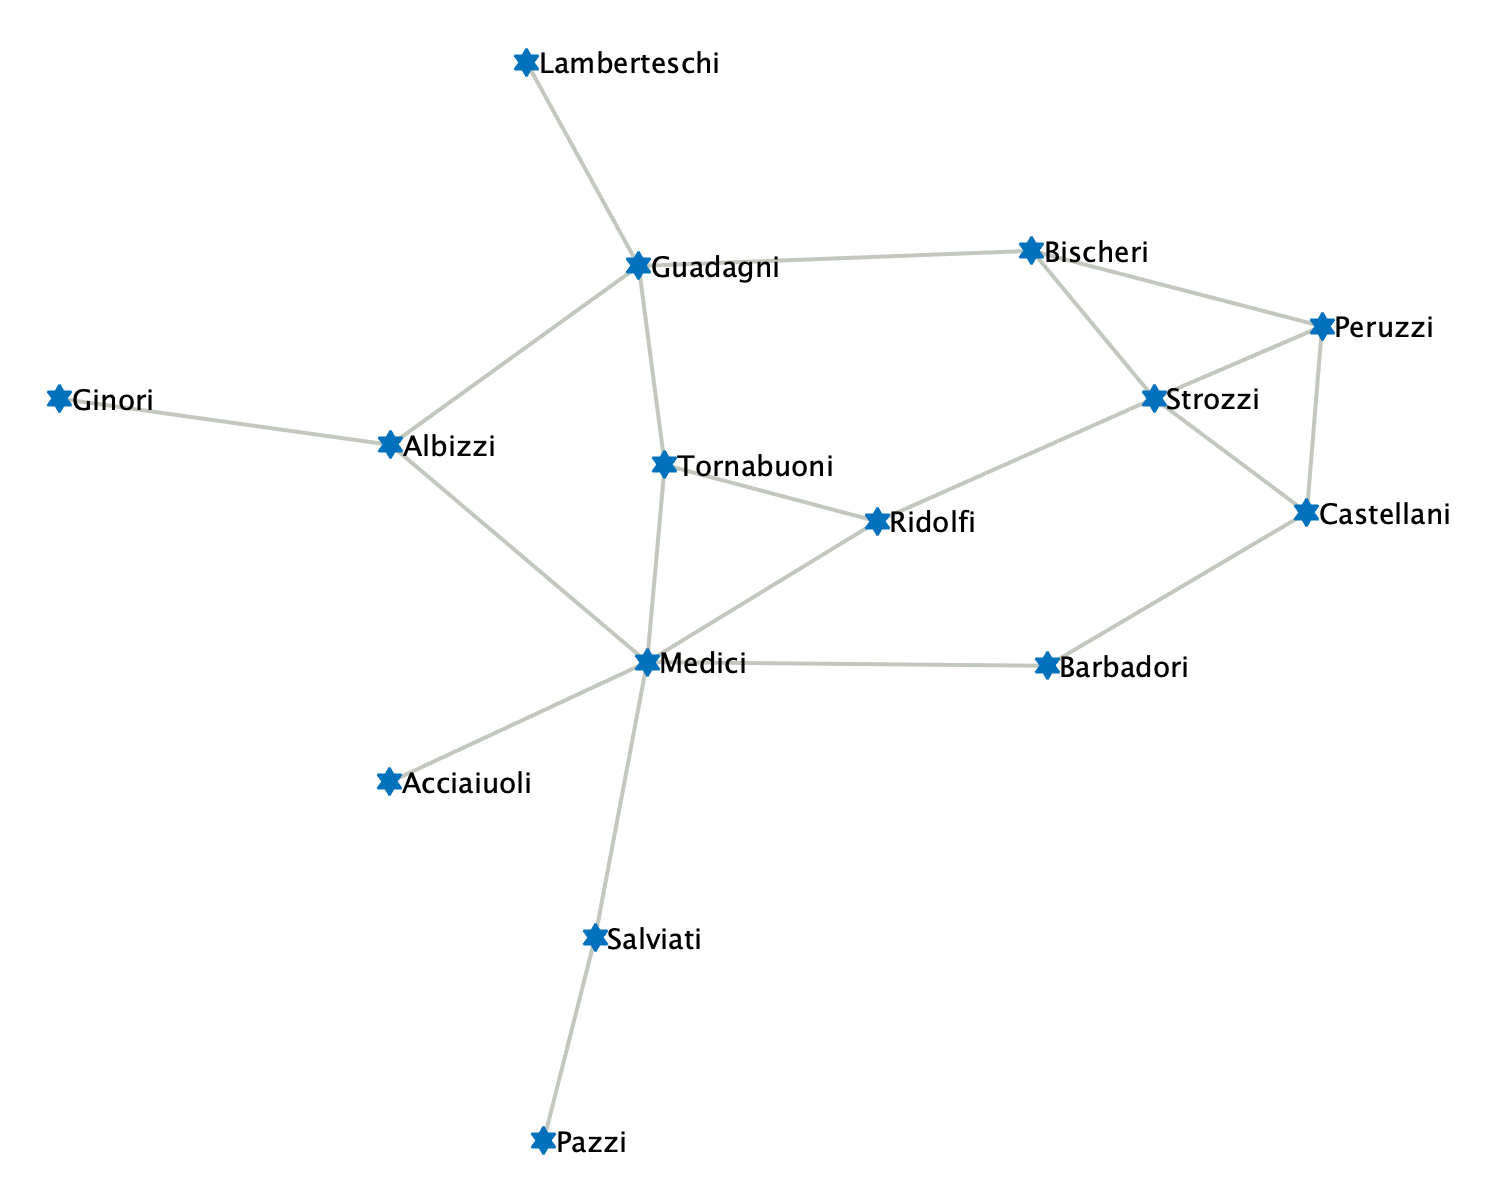
\includegraphics[scale=.19]{../Figures/introP0.png}
        \label{fig:florentineFamilies}
    \end{figure}
\end{frame}

\begin{frame}{Florentine Families with Opinions}
    \begin{figure}
        \centering
        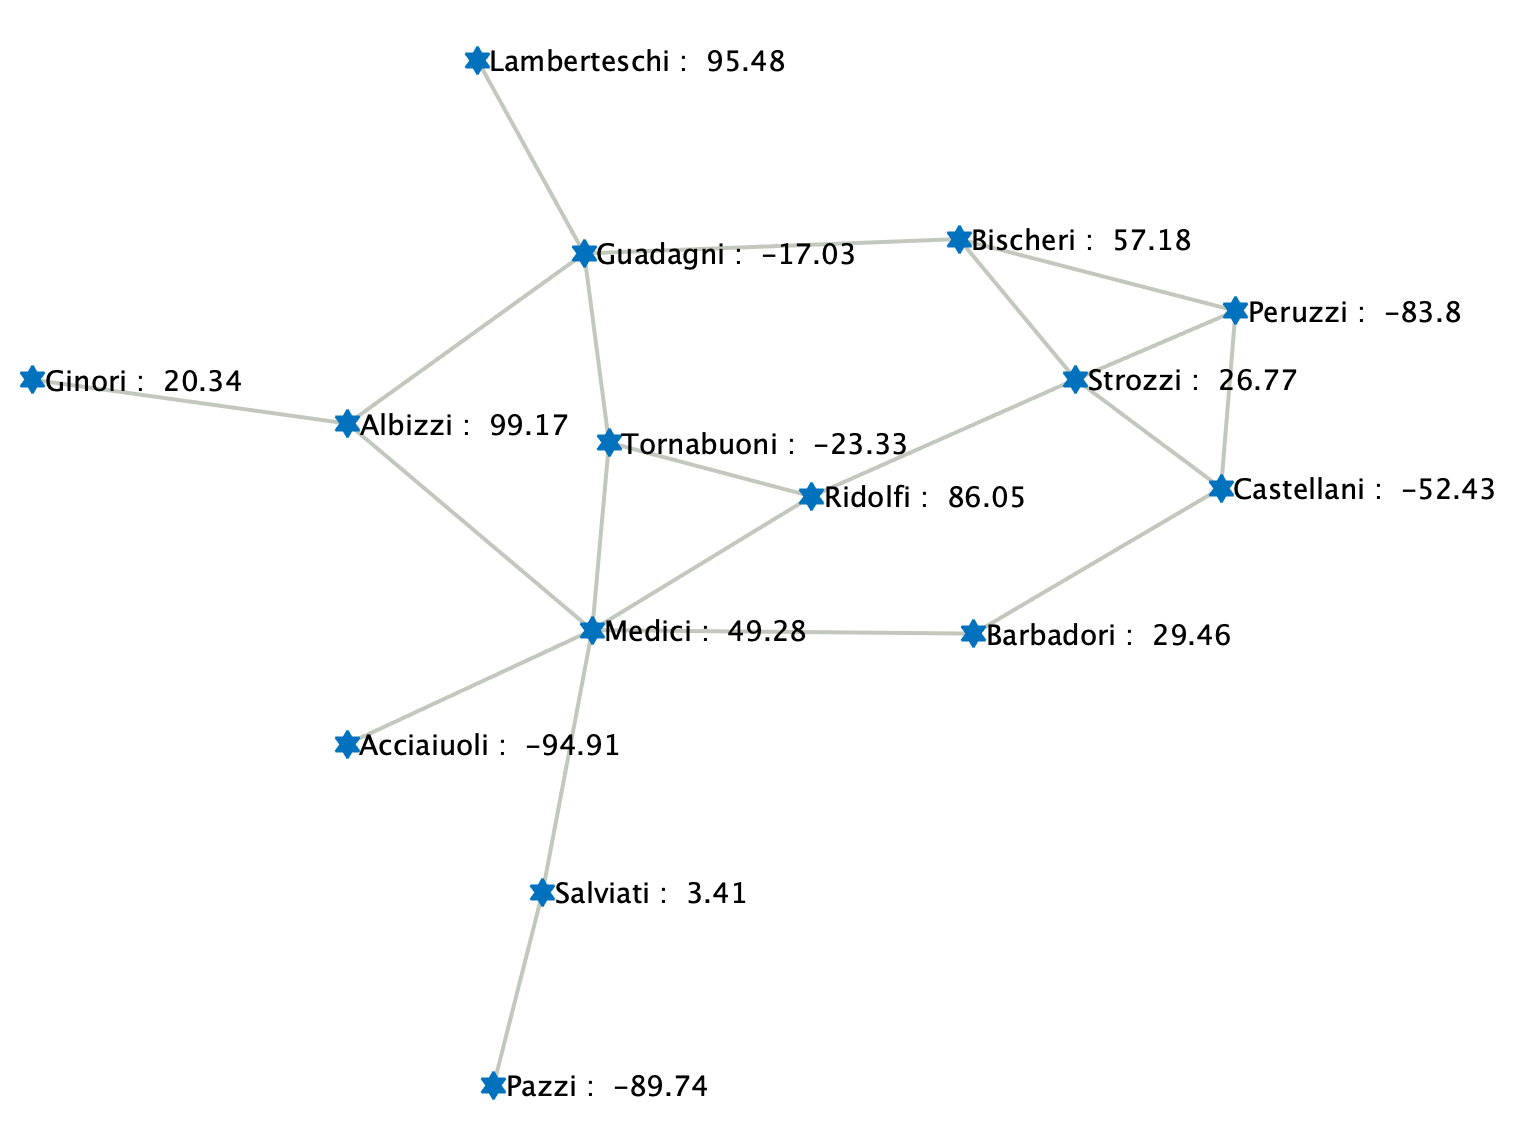
\includegraphics[scale=.19]{../Figures/introP1.png}
        \label{fig:florentineFamilies}
    \end{figure}
\end{frame}

\begin{frame}{Pairwise Updates}
    \centering
    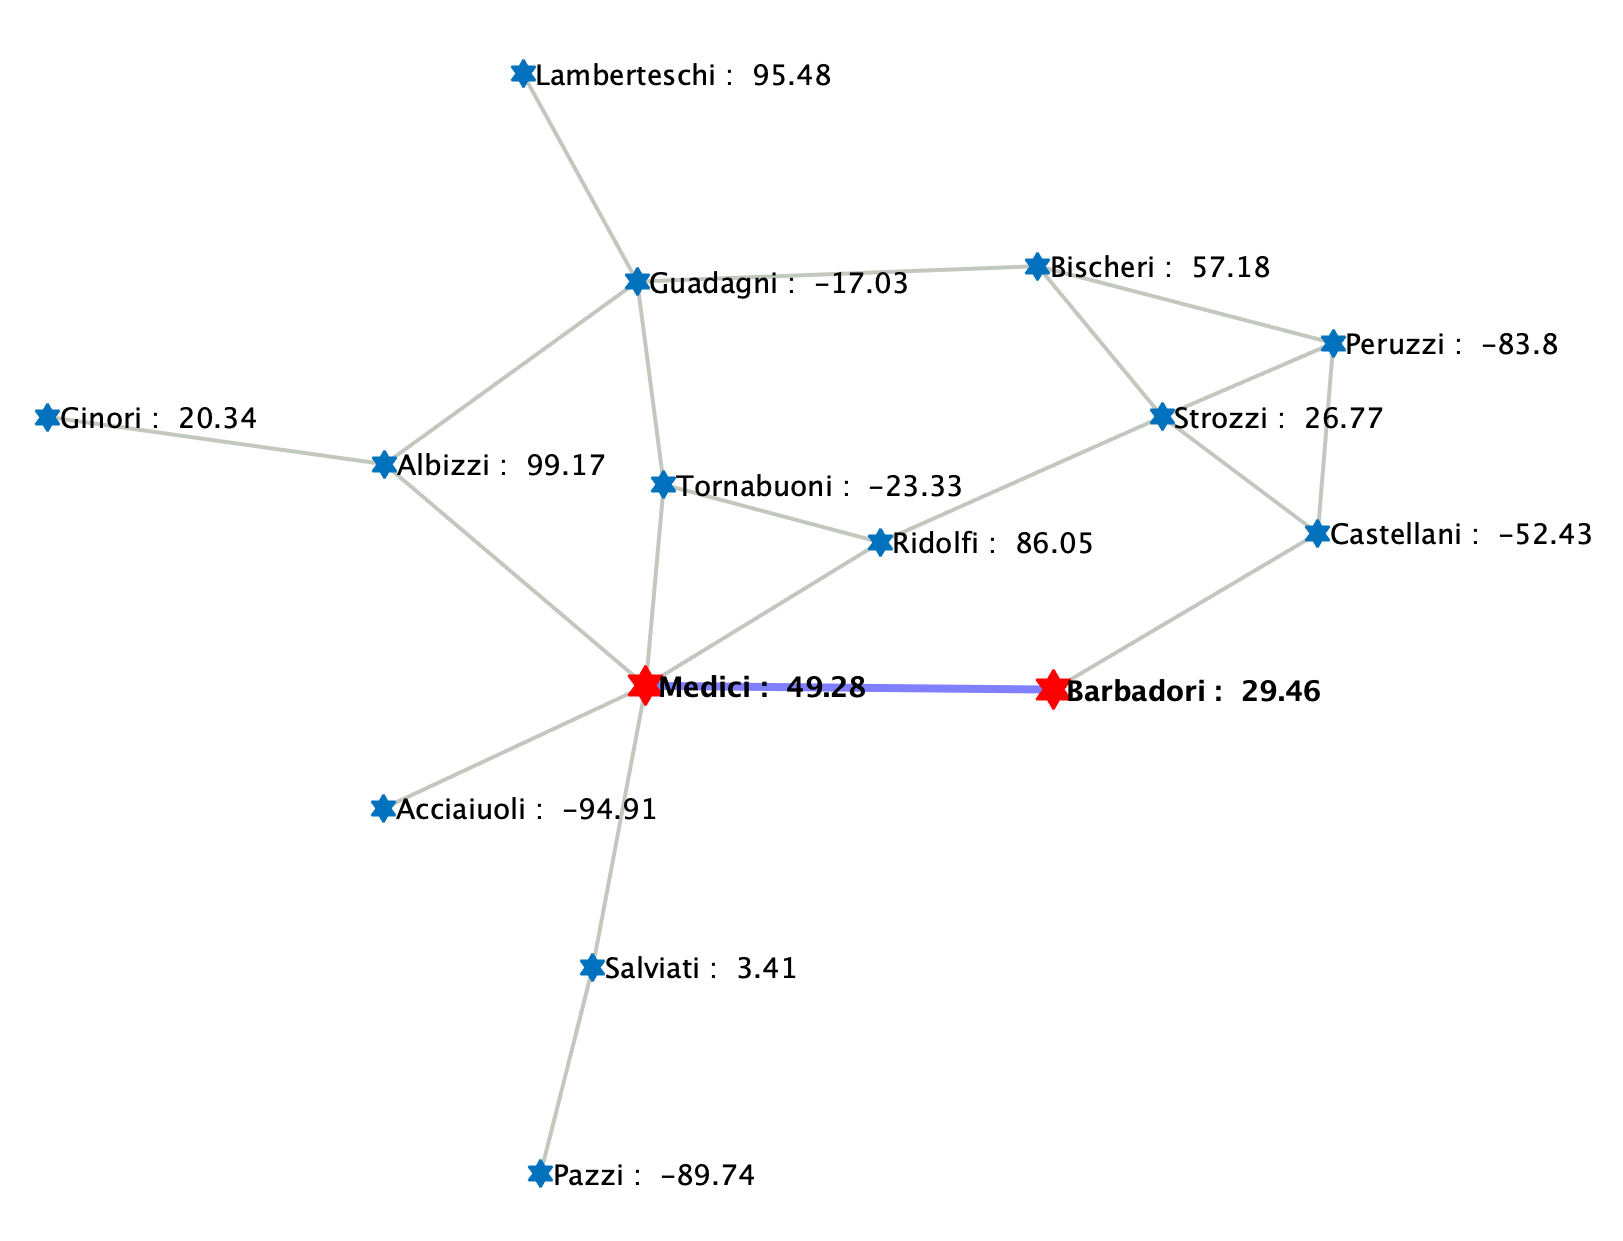
\includegraphics[scale=.18]{../Figures/introP2.png}
\end{frame}

\begin{frame}{Pairwise Updates}
    \centering
    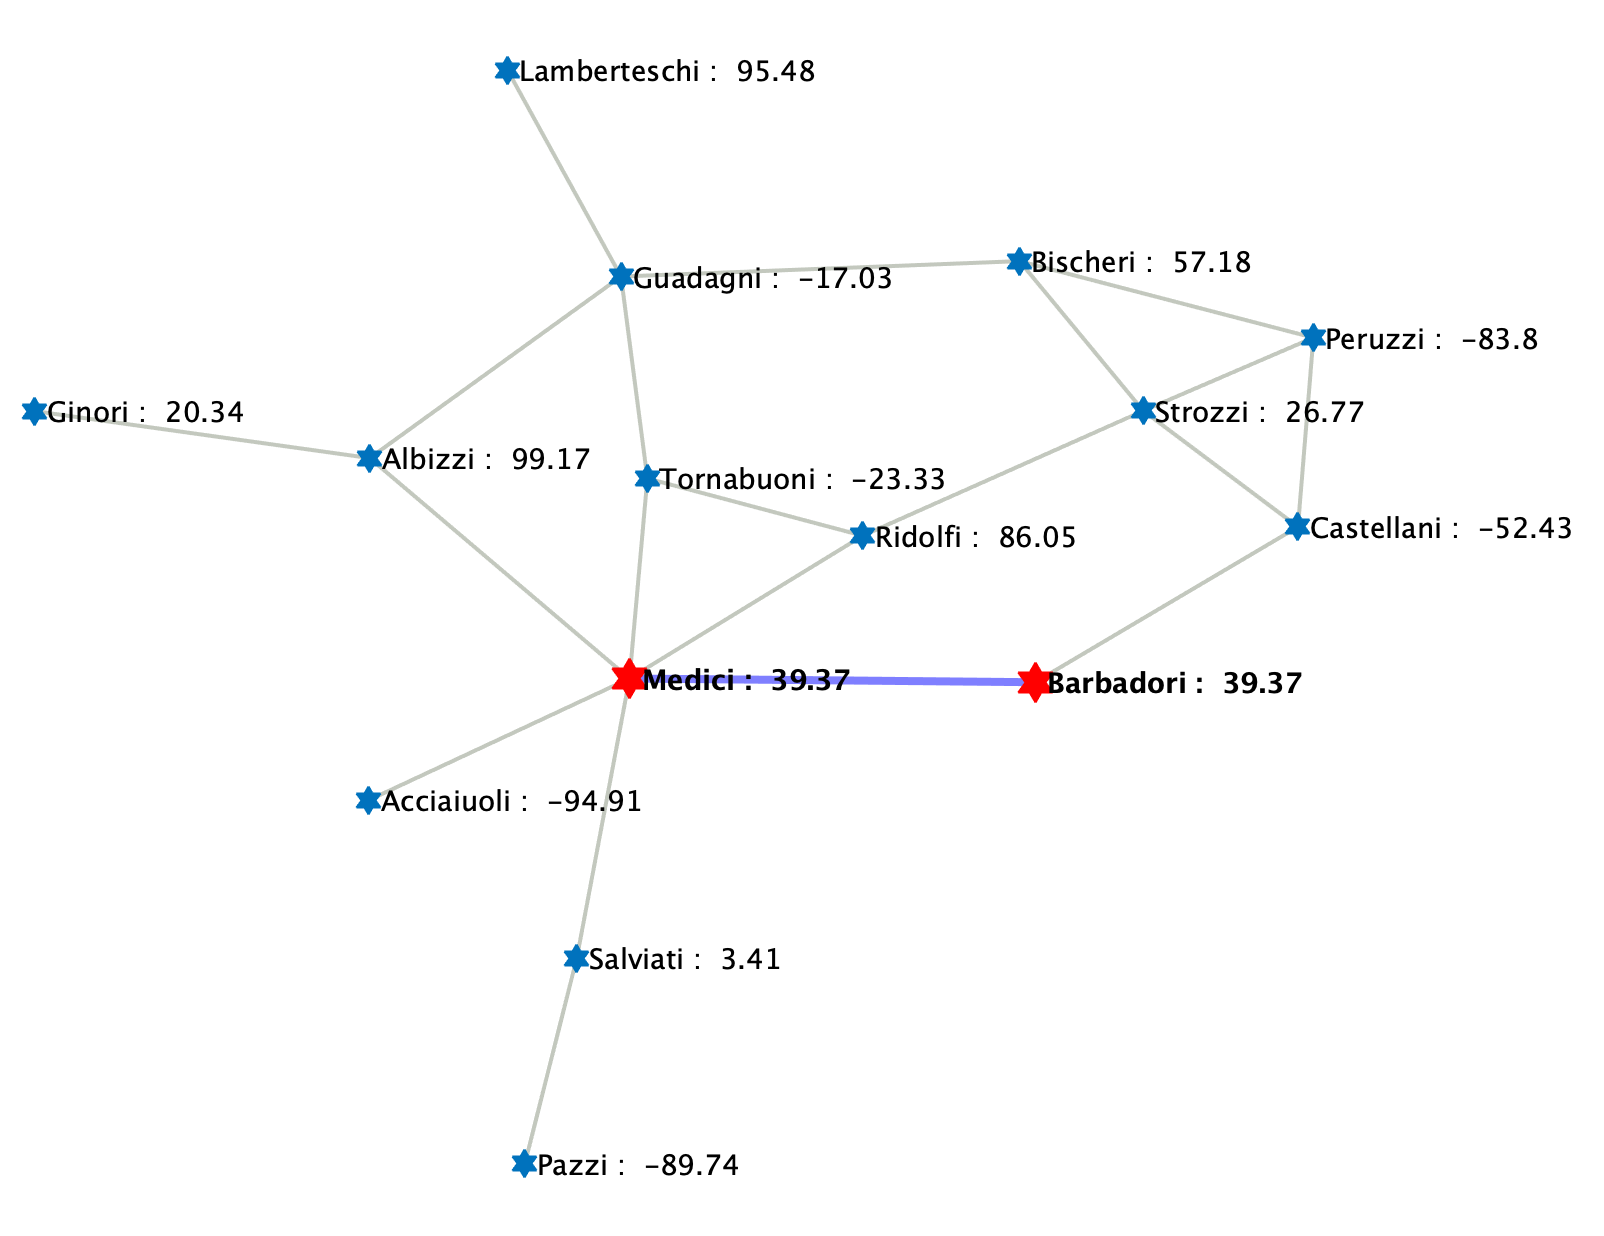
\includegraphics[scale=.18]{../Figures/introP3.png}
\end{frame}

\begin{frame}{Biased Pairwise Updates}
    \begin{overpic}[scale=.18]{../Figures/introP2.png}
                    \setlength\fboxsep{0cm}
                \put(50,12){
                \colorbox{white}{%
                \parbox{.6\linewidth}{
                \pgfsetfillopacity{1}
                \color{BrickRed}
                \small
            \begin{equation*}
                \begin{aligned}
                    &\left((49.28-29.46)^2 + (49.28-86.05)^2\right. \\
                    &+ (49.28 - (-23.33))^2 + (49.28-99.17)^2\\ &\left.+ (49.28-(-94.91))^2 
                    + (49.28-3.41)^2\right)\\
                    &+\left((29.46-49.28)^2+(29.46-(-52.43))^2\right)\\
                    &= 39500.
                \end{aligned}
                \end{equation*}
} }}
    \end{overpic}
\end{frame}

\begin{frame}{Biased Pairwise Updates}
    \begin{overpic}[scale=.18]{../Figures/introP3.png}
                \setlength\fboxsep{0cm}
                \put(50,12){
                \colorbox{white}{%
                \parbox{.6\linewidth}{
                \pgfsetfillopacity{1}
                \color{BrickRed}
                \small
                \begin{equation*}
                \begin{aligned}
                    &\left((39.37-39.37)^2 + (39.37-86.05)^2\right. \\
                    &+ (39.37 - (-23.33))^2 + (39.37-99.17)^2\\ &\left.+ (39.37-(-94.91))^2 
                    + (39.37-3.41)^2\right)\\
                    &+\left((39.37-39.37)^2+(39.37-(-52.43))^2\right)\\
                    &= 37438.
                \end{aligned}
                \end{equation*}
} }}
    \end{overpic}
\end{frame}

%\begin{frame}{Biased Pairwise Updates}
%    \begin{overpic}[scale=.18]{../Figures/introP4.png}
%                \setlength\fboxsep{0cm}
%                \put(50,12){
%                \colorbox{white}{%
%                \parbox{.6\linewidth}{
%                \pgfsetfillopacity{1}
%                \color{BrickRed}
%                \small
%                \begin{equation*}
%                \begin{aligned}
%                    &\left((26.77-(-83.8))^2 + (26.77-57.18)^2\right. \\
%                    &\left.+ (26.77 - 86.05)^2 + (26.77-(-52.43))^2\right)\\
%                    &+\left((-83.8-26.77)^2+(-83.8-57.18)^2\right.\\
%                    &\left.+(-83.8-(-52.43))^2\right)\\
%                    &= 56022.
%                \end{aligned}
%                \end{equation*}
%} }}
%    \end{overpic}
%
%\end{frame}
%
%\begin{frame}{Biased Pairwise Updates}
%    \begin{overpic}[scale=.18]{../Figures/introP5.png}
%                \setlength\fboxsep{0cm}
%                \put(49,12){
%                \colorbox{white}{%
%                \parbox{.6\linewidth}{
%                \pgfsetfillopacity{1}
%                \color{BrickRed}
%                \small
%                \begin{equation*}
%                \begin{aligned}
%                    &\left((-28.52-(-28.52))^2 + (-28.52-57.18)^2\right. \\
%                    &\left.+ (-28.52 - 86.05)^2 + (-28.52-(-52.43))^2\right)\\
%                    &+\left((-28.52-(-28.52))^2+(-28.52-57.18)^2\right.\\
%                    &\left.+(-28.52-(-52.43))^2\right)\\
%                    &= 28959.
%                \end{aligned}
%                \end{equation*}
%} }}
%    \end{overpic}
%\end{frame}

\begin{frame}{Biased Pairwise Updates}
    \begin{overpic}[scale=.18]{../Figures/introP6.png}
                \setlength\fboxsep{0cm}
                \put(50,13){
                \colorbox{white}{%
                \parbox{.6\linewidth}{
                \pgfsetfillopacity{1}
                \color{BrickRed}
                \small
                \begin{equation*}
                \begin{aligned}
                    &\left((-17.03-(-23.33))^2 + (-17.03-97.17)^2\right. \\
                    &\left.+ (-17.03 - 95.48)^2 + (-17.03-57.18)^2\right)\\
                    &+\left((-23.33-(-17.03))^2+(-23.33-62.71)^2\right.\\
                    &\left.+(-23.33-62.17)^2\right)\\
                    &= 46000.
                \end{aligned}
                \end{equation*}
} }}
    \end{overpic}
\end{frame}

\begin{frame}{Biased Pairwise Updates}
    \begin{overpic}[scale=.18]{../Figures/introP7.png}
                \put(37,52) {
                    \color{BrickRed}
                    \Huge
                    x
                }
                \setlength\fboxsep{0cm}
                \put(50,14){
                \colorbox{white}{%
                \parbox{.6\linewidth}{
                \pgfsetfillopacity{1}
                \color{BrickRed}
                \small
                \begin{equation*}
                \begin{aligned}
                    &\left((-20.18-(-20.18))^2 + (-20.18-97.17)^2\right. \\
                    &\left.+ (-20.18 - 95.48)^2 + (-20.18-57.18)^2\right)\\
                    &+\left((-20.18-(-20.18))^2\right.\\
                    &\left.+(-20.18-62.71)^2+(-20.18-62.17)^2\right)\\
                    &= 46785.
                \end{aligned}
                \end{equation*}
} }}
    \end{overpic}
\end{frame}

\begin{frame}{Successful Biased Pairwise Updates}
    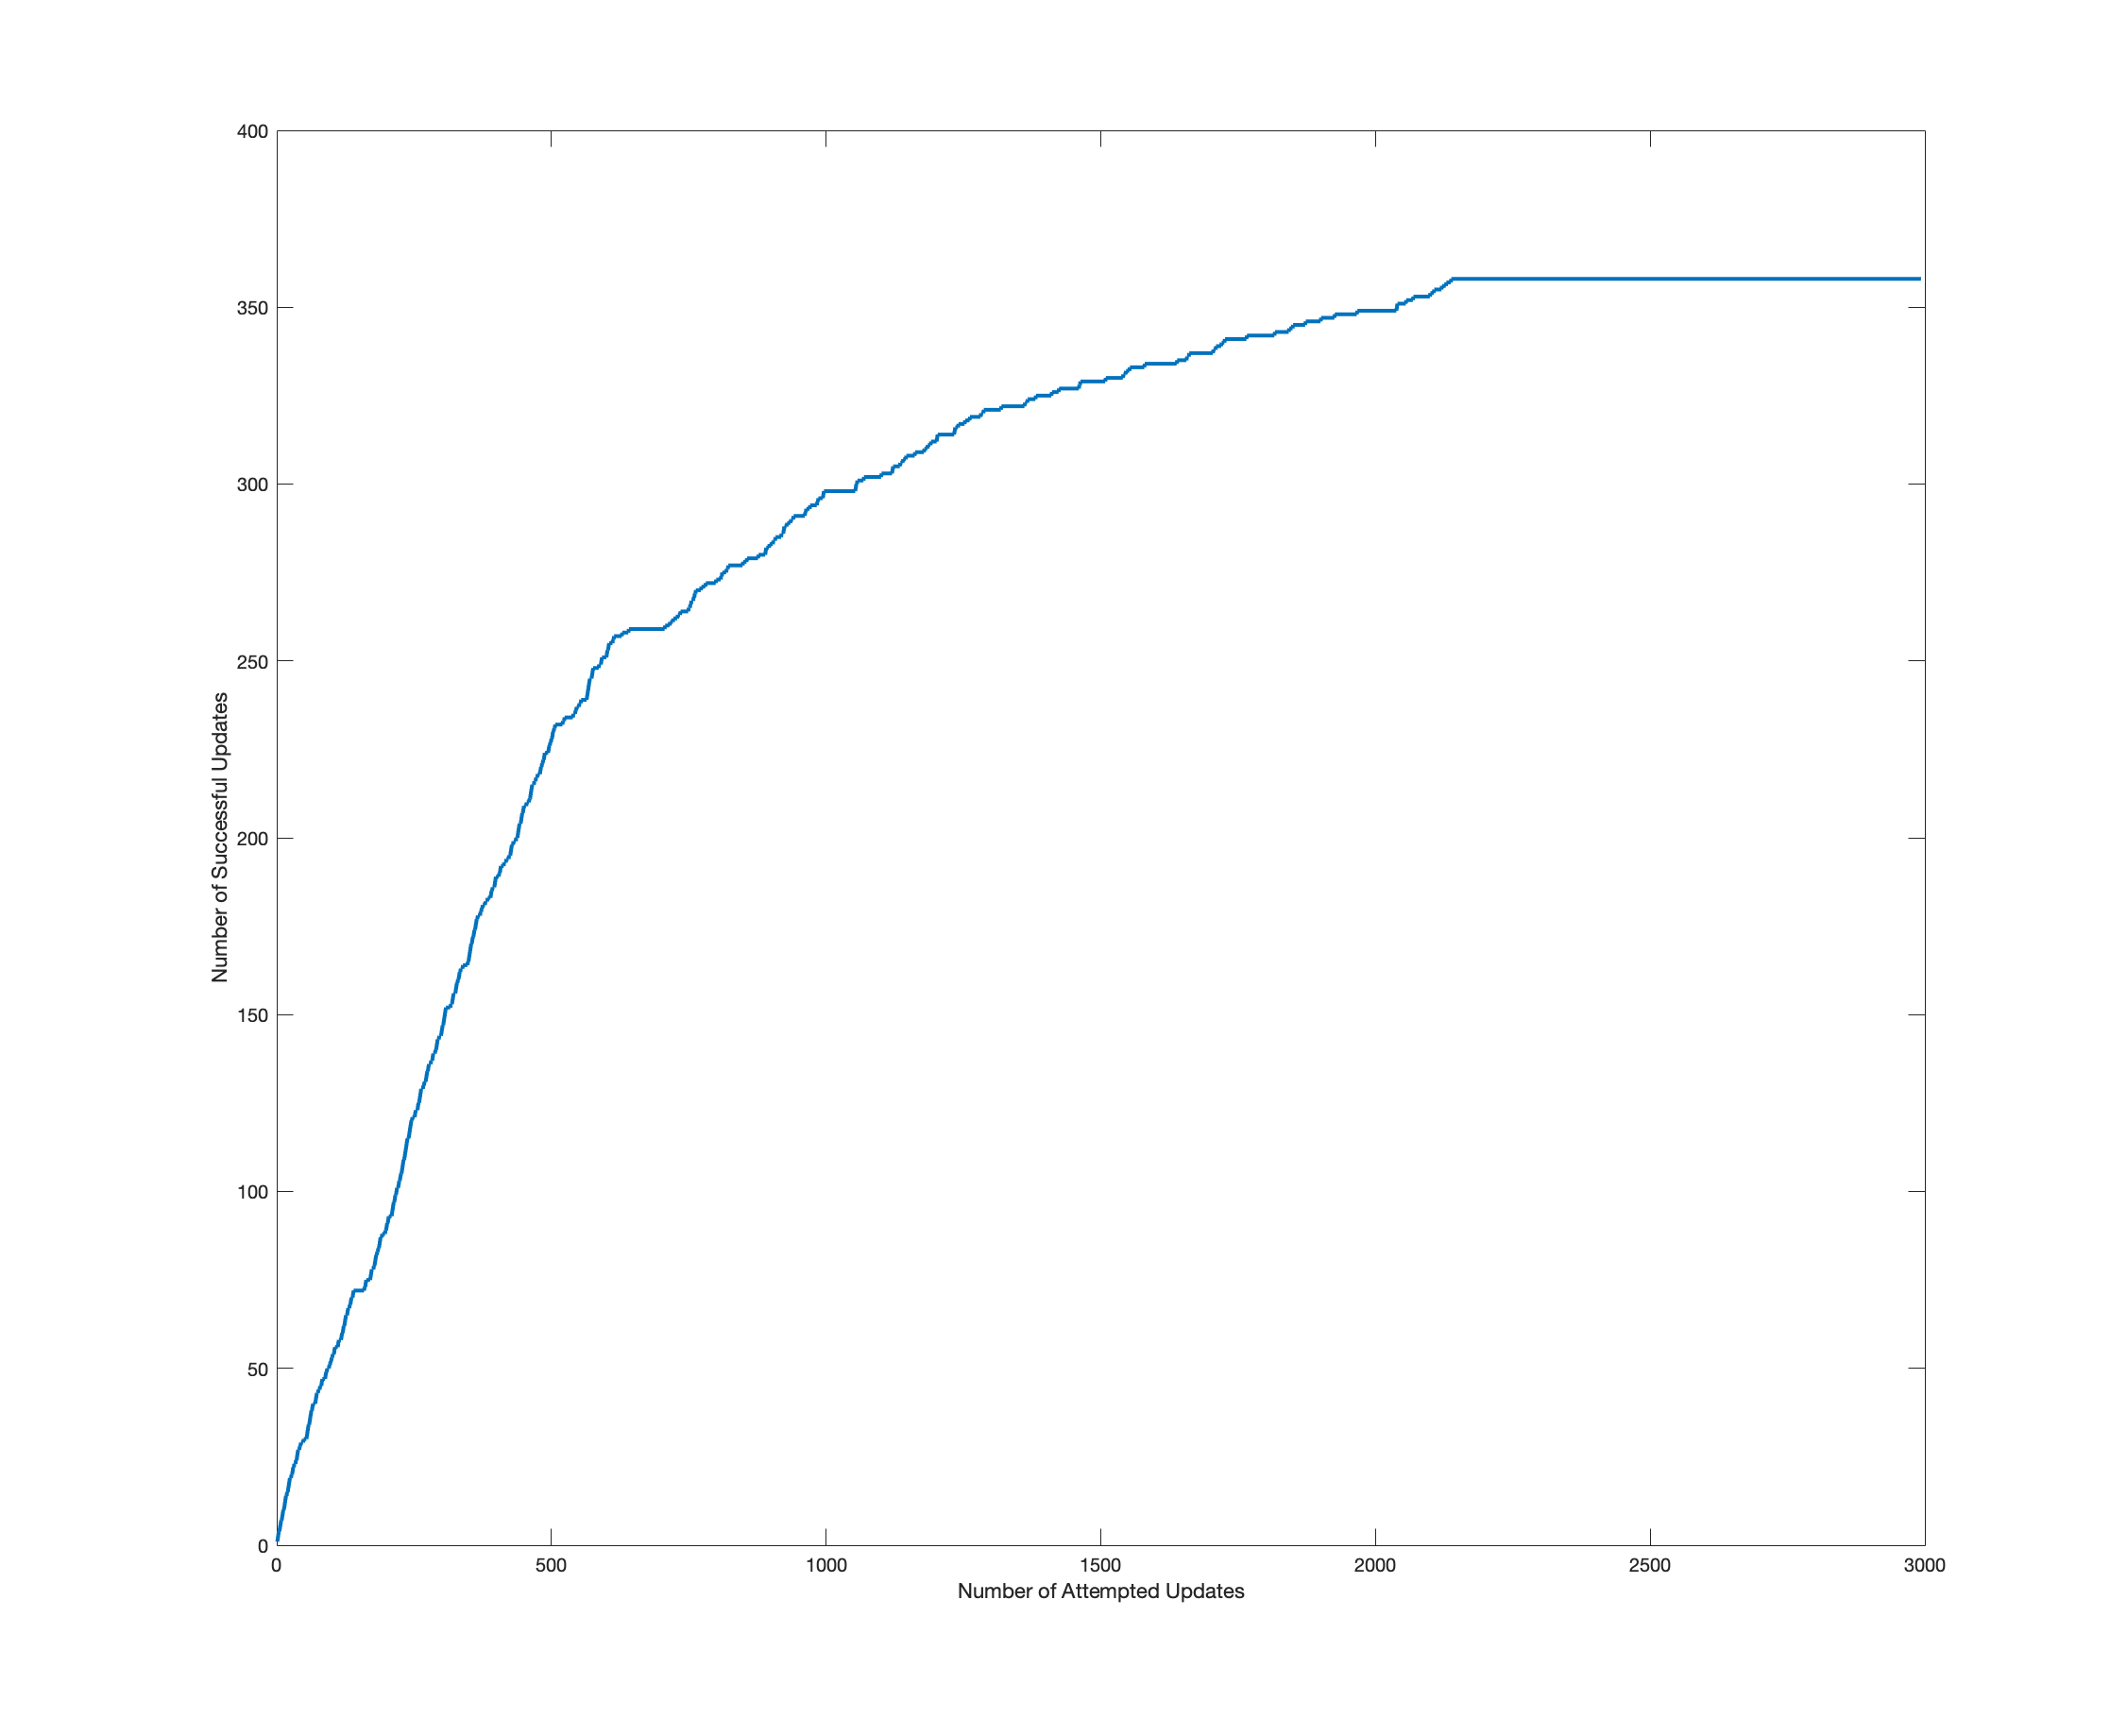
\includegraphics[scale=.13]{../Figures/introP8.png}
\end{frame}

\begin{frame}{Successful Biased Pairwise Updates}
    \begin{overpic}[scale=.13]{../Figures/introP8.png}
                \put(70,69){
                \large
                \color{BrickRed}

                deadlock
                
                }
    \end{overpic}
\end{frame}

\begin{frame}{Consensus Error - Biased Pairwise Updates}
    \begin{overpic}[scale=.13]{../Figures/introP9.png}
        \huge
                \put(50,50){
                
                $
                    \frac{\|x(k)-\bar{x}_{0}\|_2}{\|x_0-\bar{x}_{0}\|_2}
                $
                
                }
    \end{overpic}
\end{frame}

\begin{frame}{Biased Pairwise Updates - Steady state}
\centering
    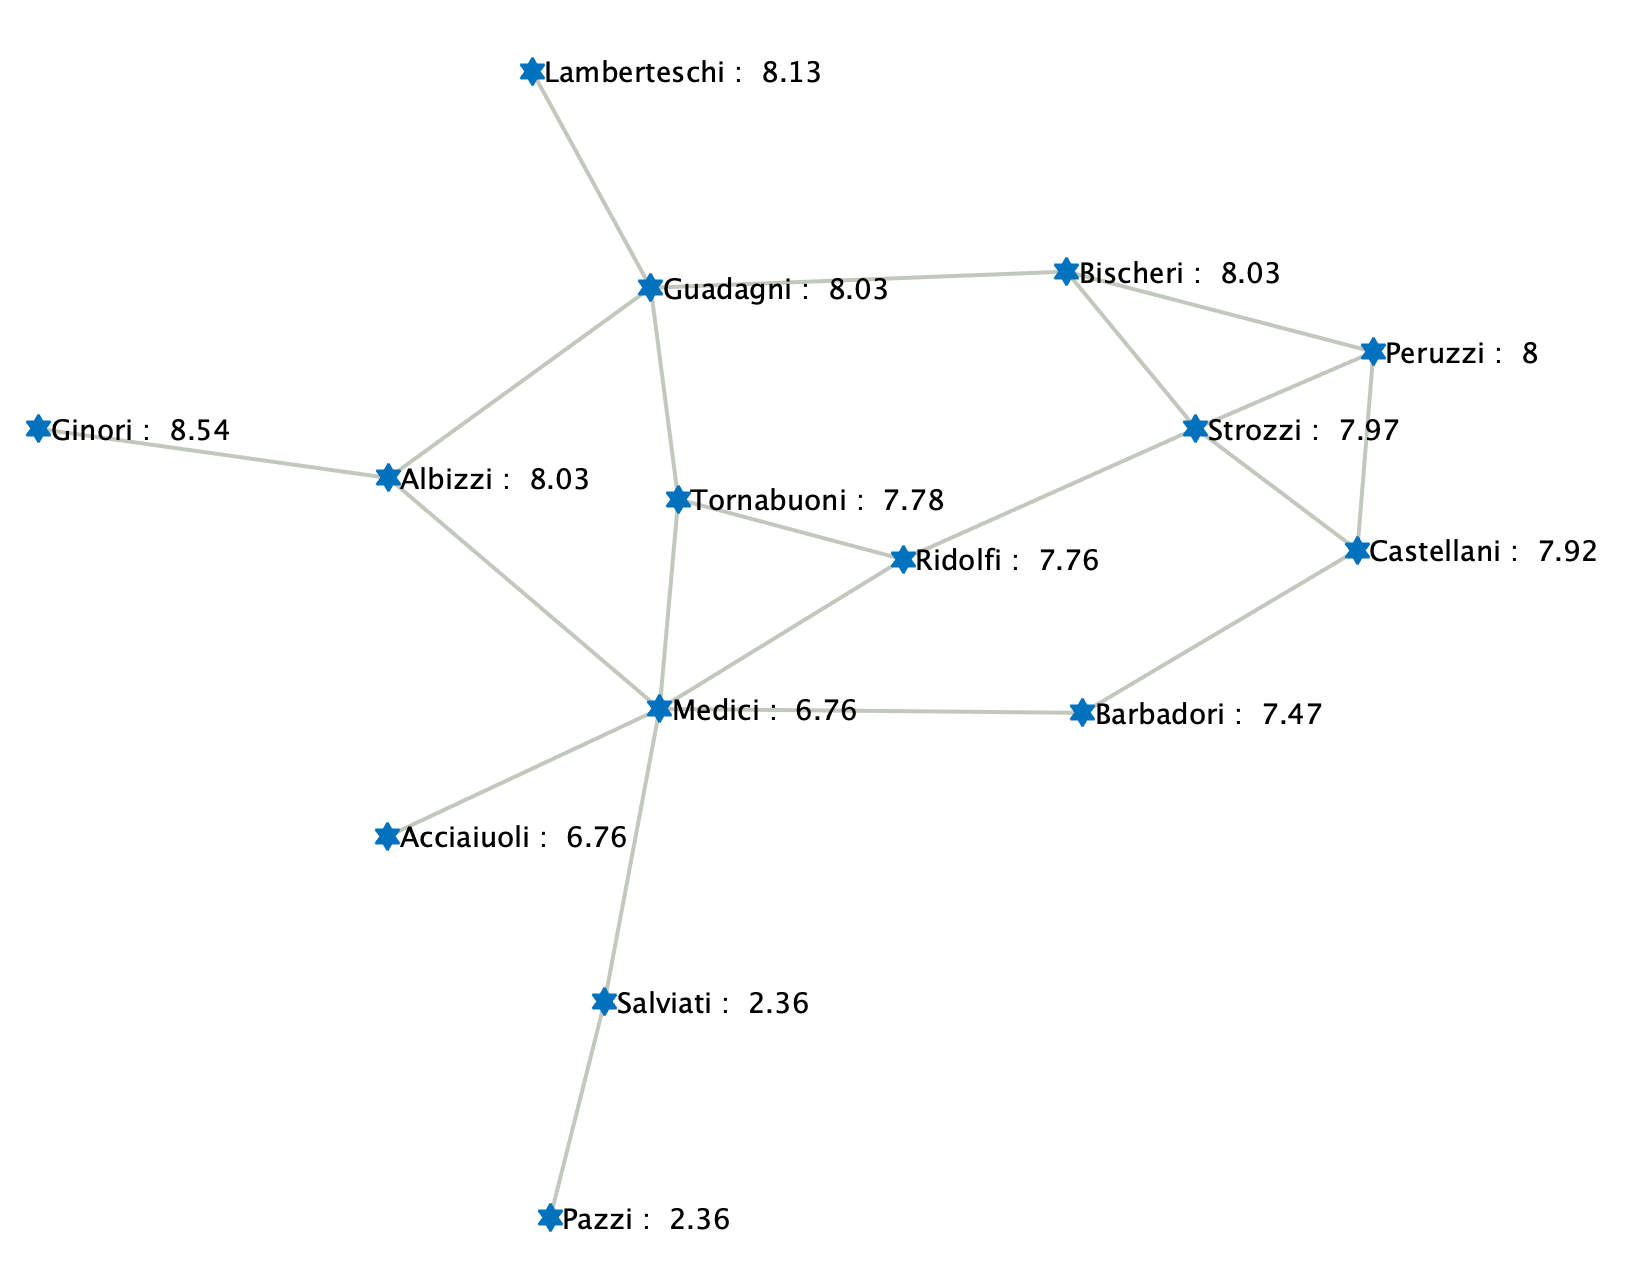
\includegraphics[scale=.18]{../Figures/introP10.png}
\end{frame}

\begin{frame}{Biased Triple-wise Updates}
    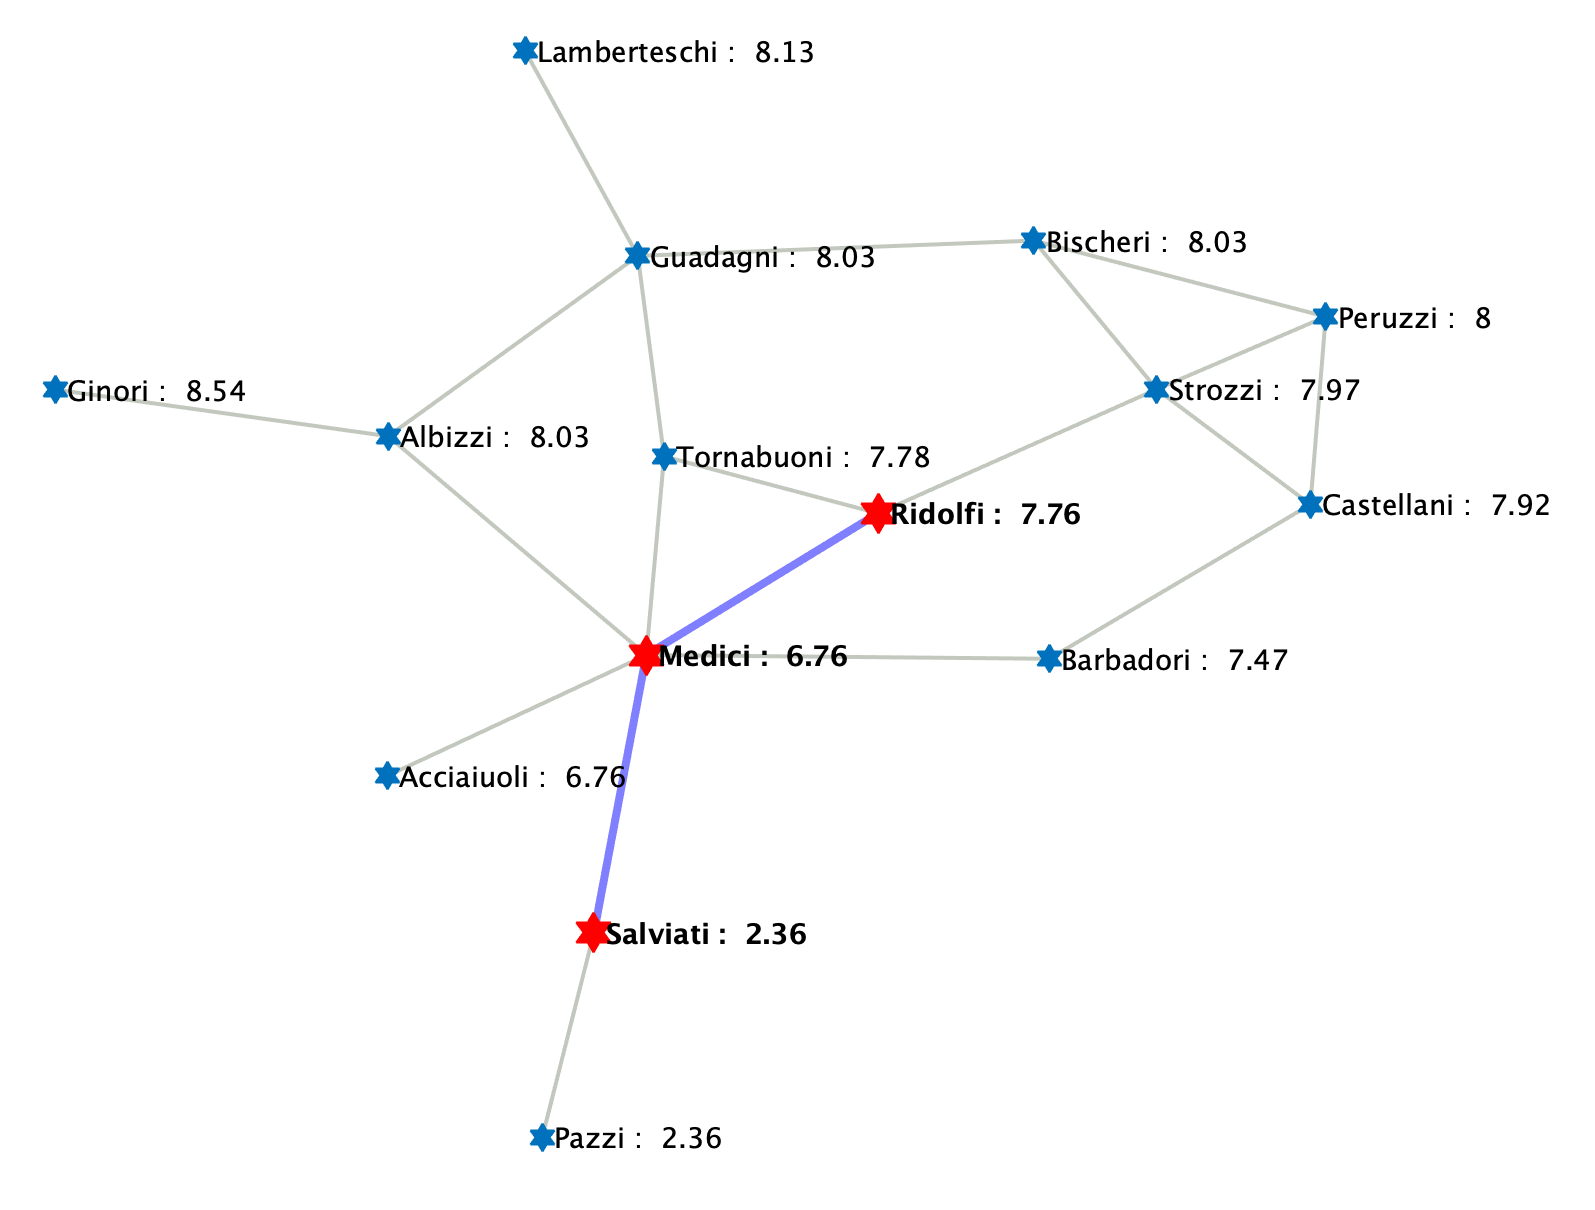
\includegraphics[scale=.18]{../Figures/introP32.png}
\end{frame}

\begin{frame}{Biased Triple-wise Updates}
    \begin{overpic}[scale=.18]{../Figures/introP32.png}
                \setlength\fboxsep{0cm}
                \put(50,13){
                \colorbox{white}{%
                \parbox{.6\linewidth}{
                \pgfsetfillopacity{1}
                \color{BrickRed}
                \scriptsize
                \begin{equation*}
                \begin{aligned}
                    &\left((2.36-6.76)^2 + (2.36-2.36)^2\right)\\
                    &+\left((6.76-2.36)^2 + (6.76-6.76)^2\right.\\
                    &+\left.(6.76-8.03)^2 + (6.76-7.78)^2\right.\\
                    &+\left.(6.76-7.76)^2 + (6.76-7.47)^2\right)\\
                    &+\left((7.76-6.76)^2 + (7.76-7.78)^2\right.\\
                    &+\left.(7.76-7.97)^2\right)\\
                    &= 43.92
                \end{aligned}
                \end{equation*}
} }}
    \end{overpic}
\end{frame}

\begin{frame}{Biased Triple-wise Updates}
    \begin{overpic}[scale=.18]{../Figures/introP33.png}
                \setlength\fboxsep{0cm}
                \put(50,13){
                \colorbox{white}{%
                \parbox{.6\linewidth}{
                \pgfsetfillopacity{1}
                \color{BrickRed}
                \scriptsize
                \begin{equation*}
                \begin{aligned}
                    &\left((5.63-5.63)^2 + (5.63-2.36)^2\right)\\
                    &+\left((5.63-5.63)^2 + (5.63-6.76)^2\right.\\
                    &+\left.(5.63-8.03)^2 + (5.63-7.78)^2\right.\\
                    &+\left.(5.63-5.63)^2 + (6.76-7.47)^2\right)\\
                    &+\left((5.63-5.63)^2 + (5.63-7.78)^2\right.\\
                    &+\left.(5.63-7.97)^2\right)\\
                    &= 32.95
                \end{aligned}
                \end{equation*}
} }}
    \end{overpic}
\end{frame}

\begin{frame}{Successful Biased Triple-wise Updates}
    \begin{overpic}[scale=.13]{../Figures/introP34.png}
                \put(50,69){
                \color{BrickRed}
                    deadlock
                }
    \end{overpic}
\end{frame}

\begin{frame}{\small Consensus Error - Biased Triple-wise Updates}
\centering
    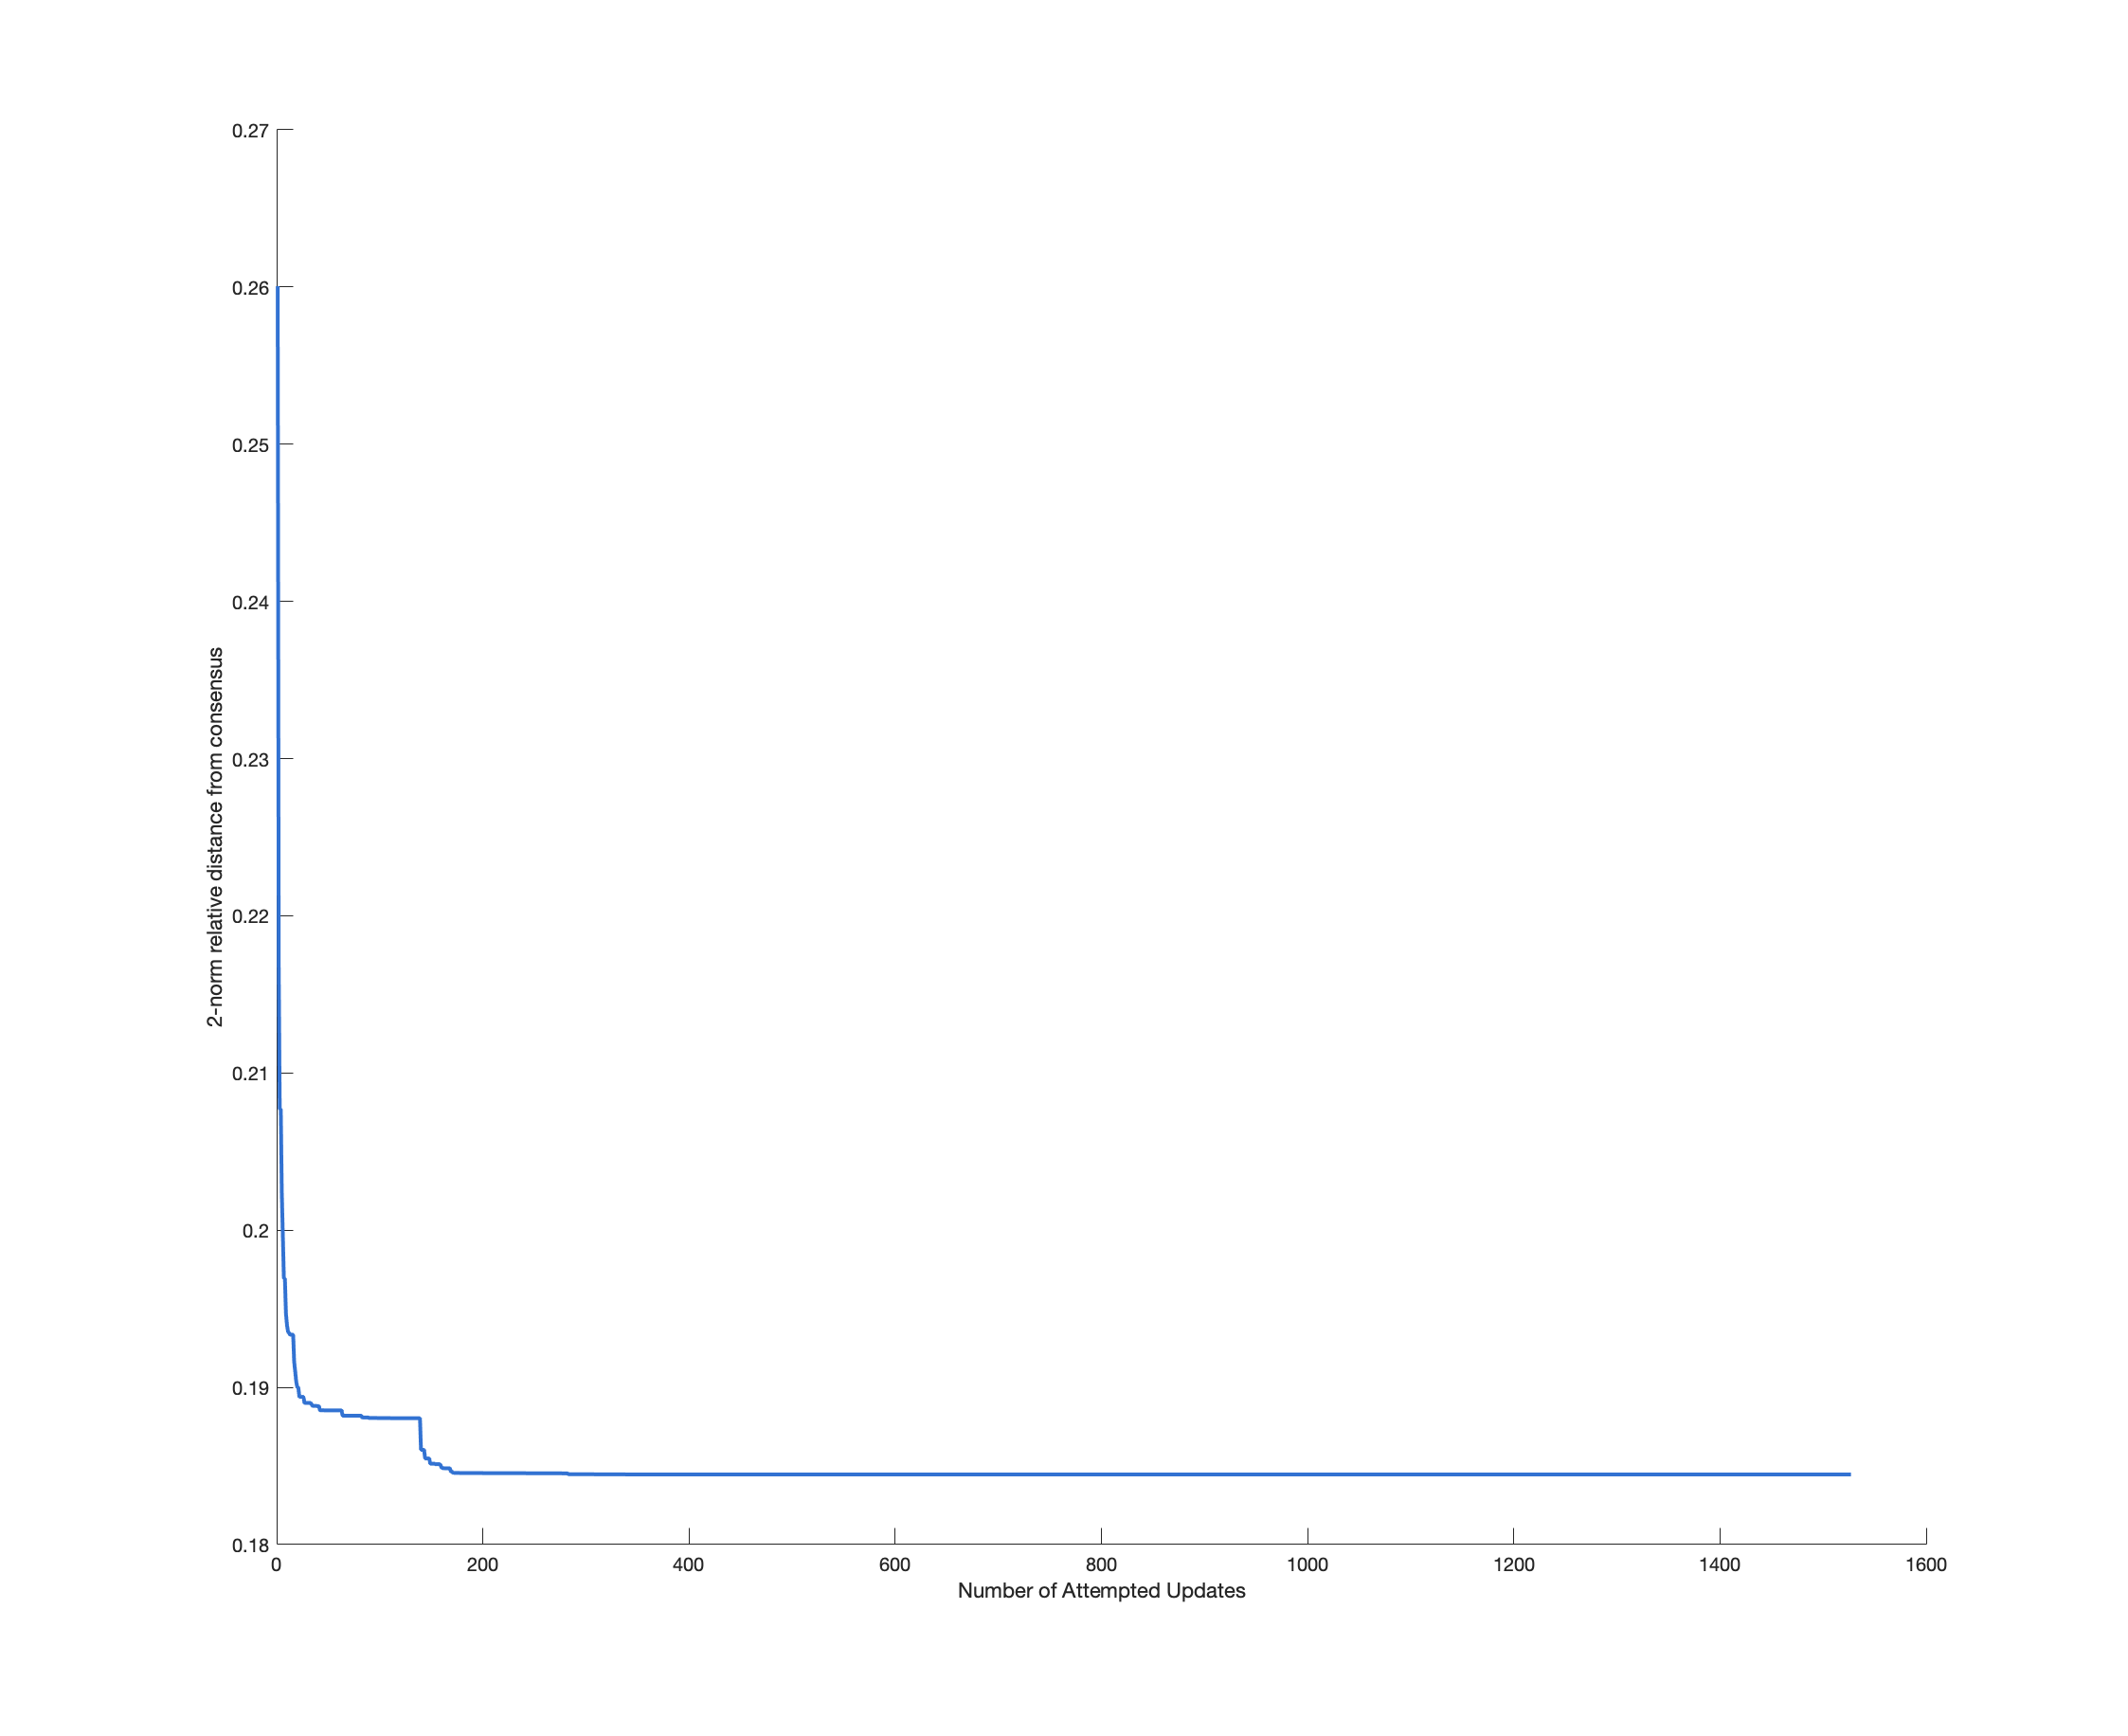
\includegraphics[scale=.13]{../Figures/introP35.png}
\end{frame}

\begin{frame}{Biased Triple-wise Updates - Steady state}
\centering
    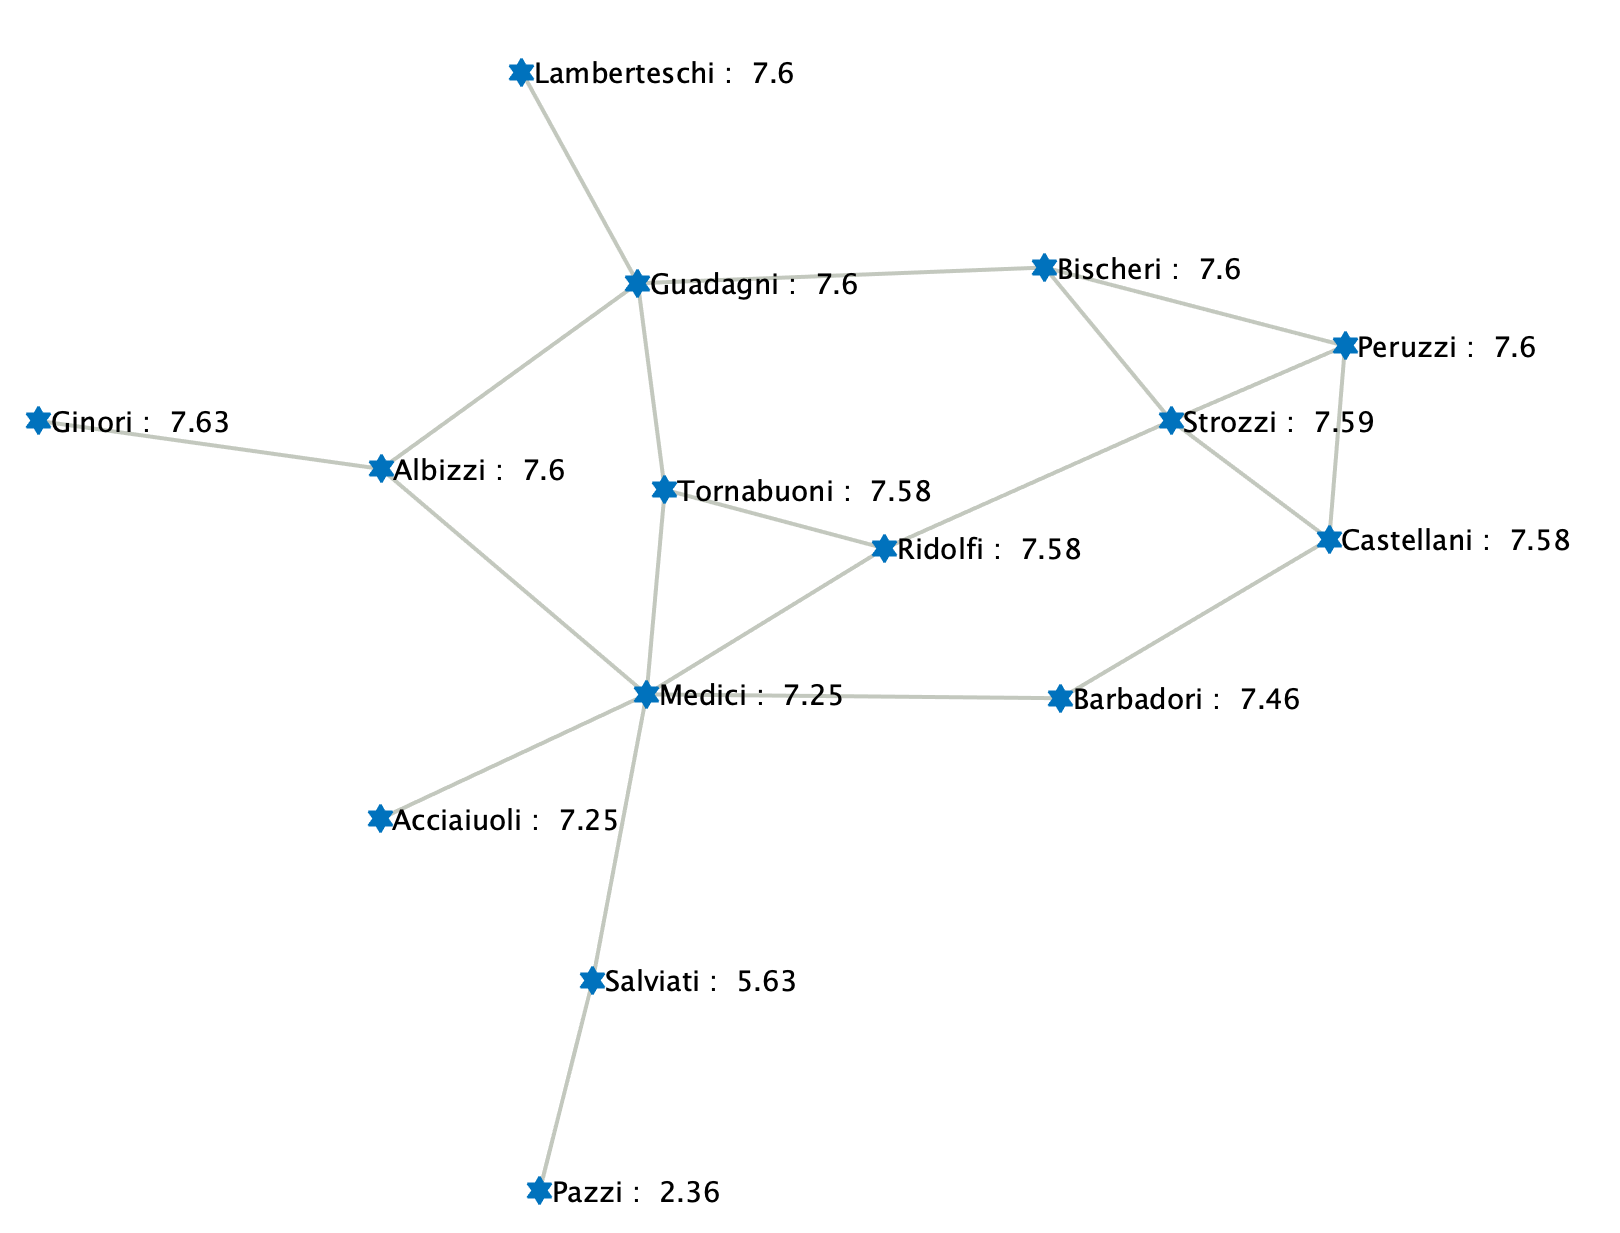
\includegraphics[scale=.18]{../Figures/introP41.png}
\end{frame}

\begin{frame}{Biased Quadruple-wise Updates}
\centering
    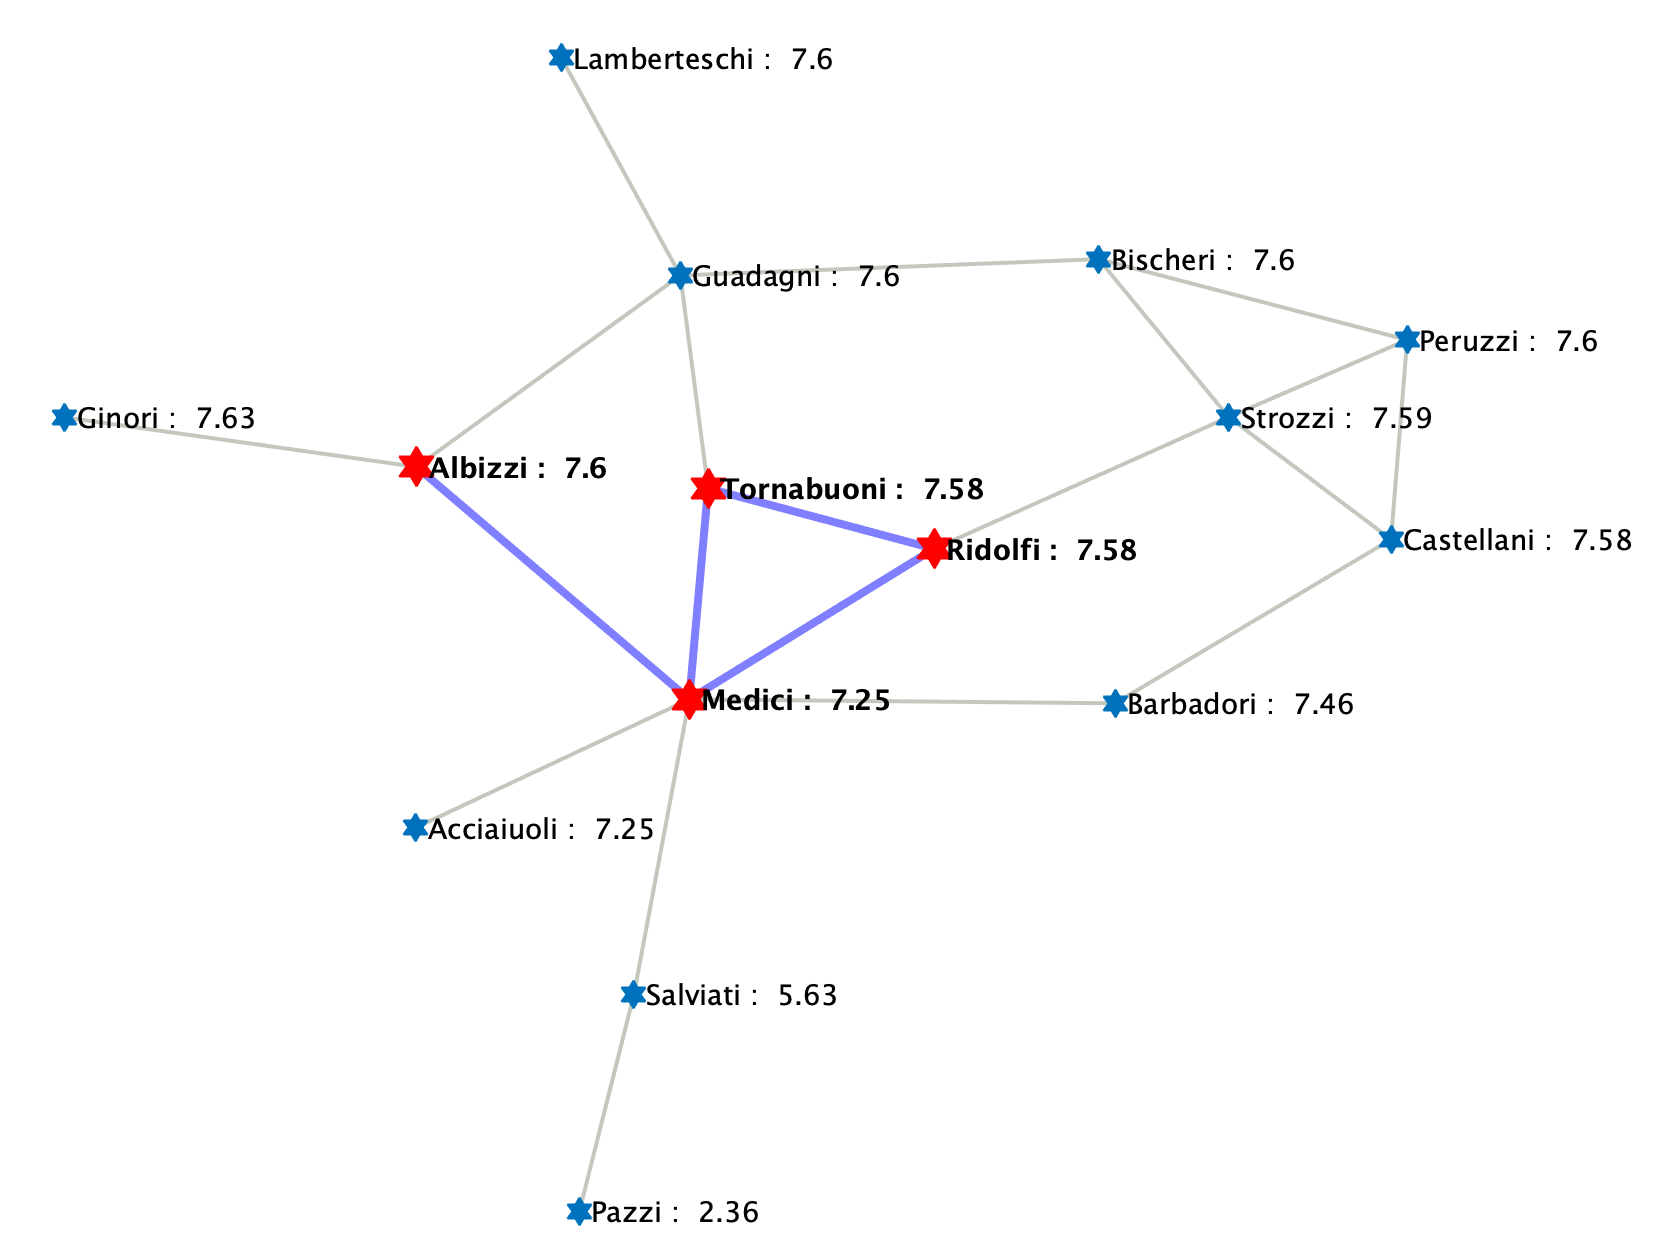
\includegraphics[scale=.18]{../Figures/introP42.png}
\end{frame}

\begin{frame}{Biased Quadruple-wise Updates}
\begin{overpic}[scale=.18]{../Figures/introP43.png}
\put(37.75,38) {
\Huge
\color{BrickRed}
X
}
\end{overpic}
\end{frame}

\begin{frame}{Biased Quadruple-wise Updates}
\centering
    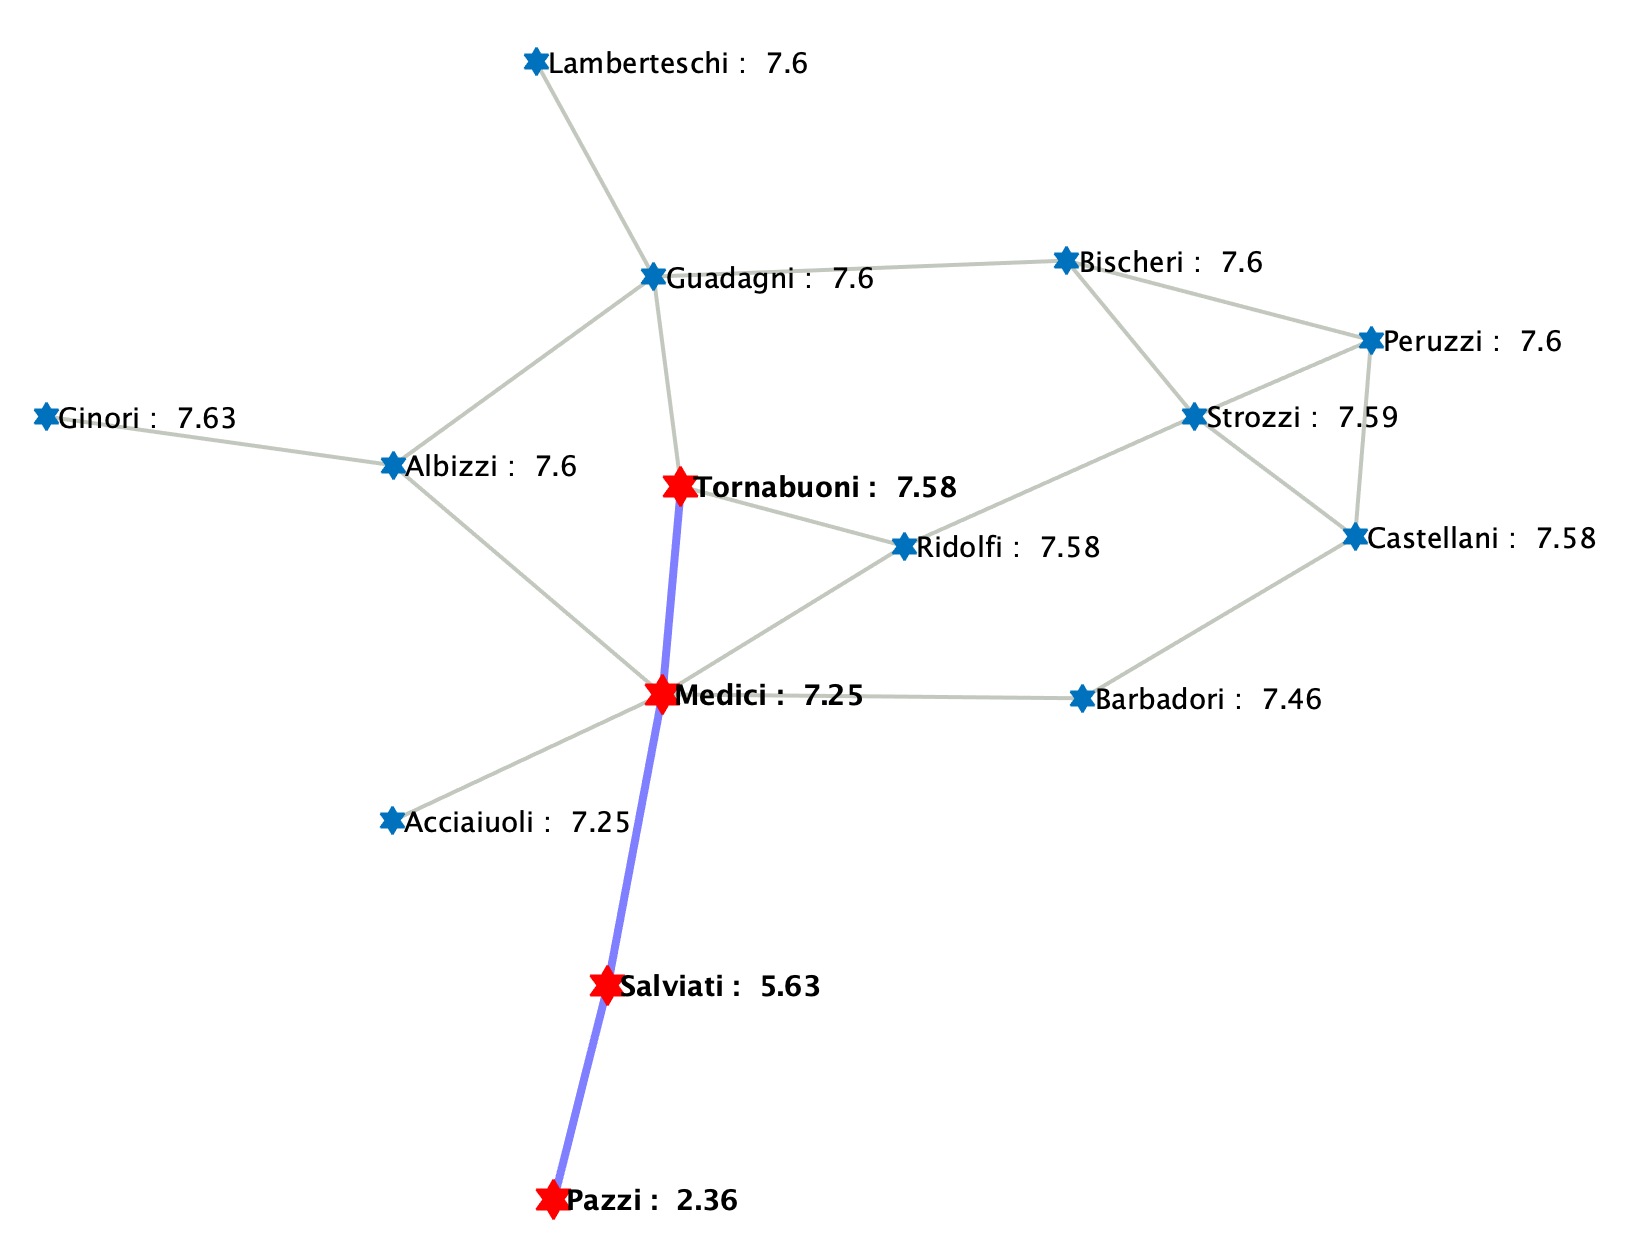
\includegraphics[scale=.18]{../Figures/introP44.png}
\end{frame}

\begin{frame}{Biased Quadruple-wise Updates}
\centering
    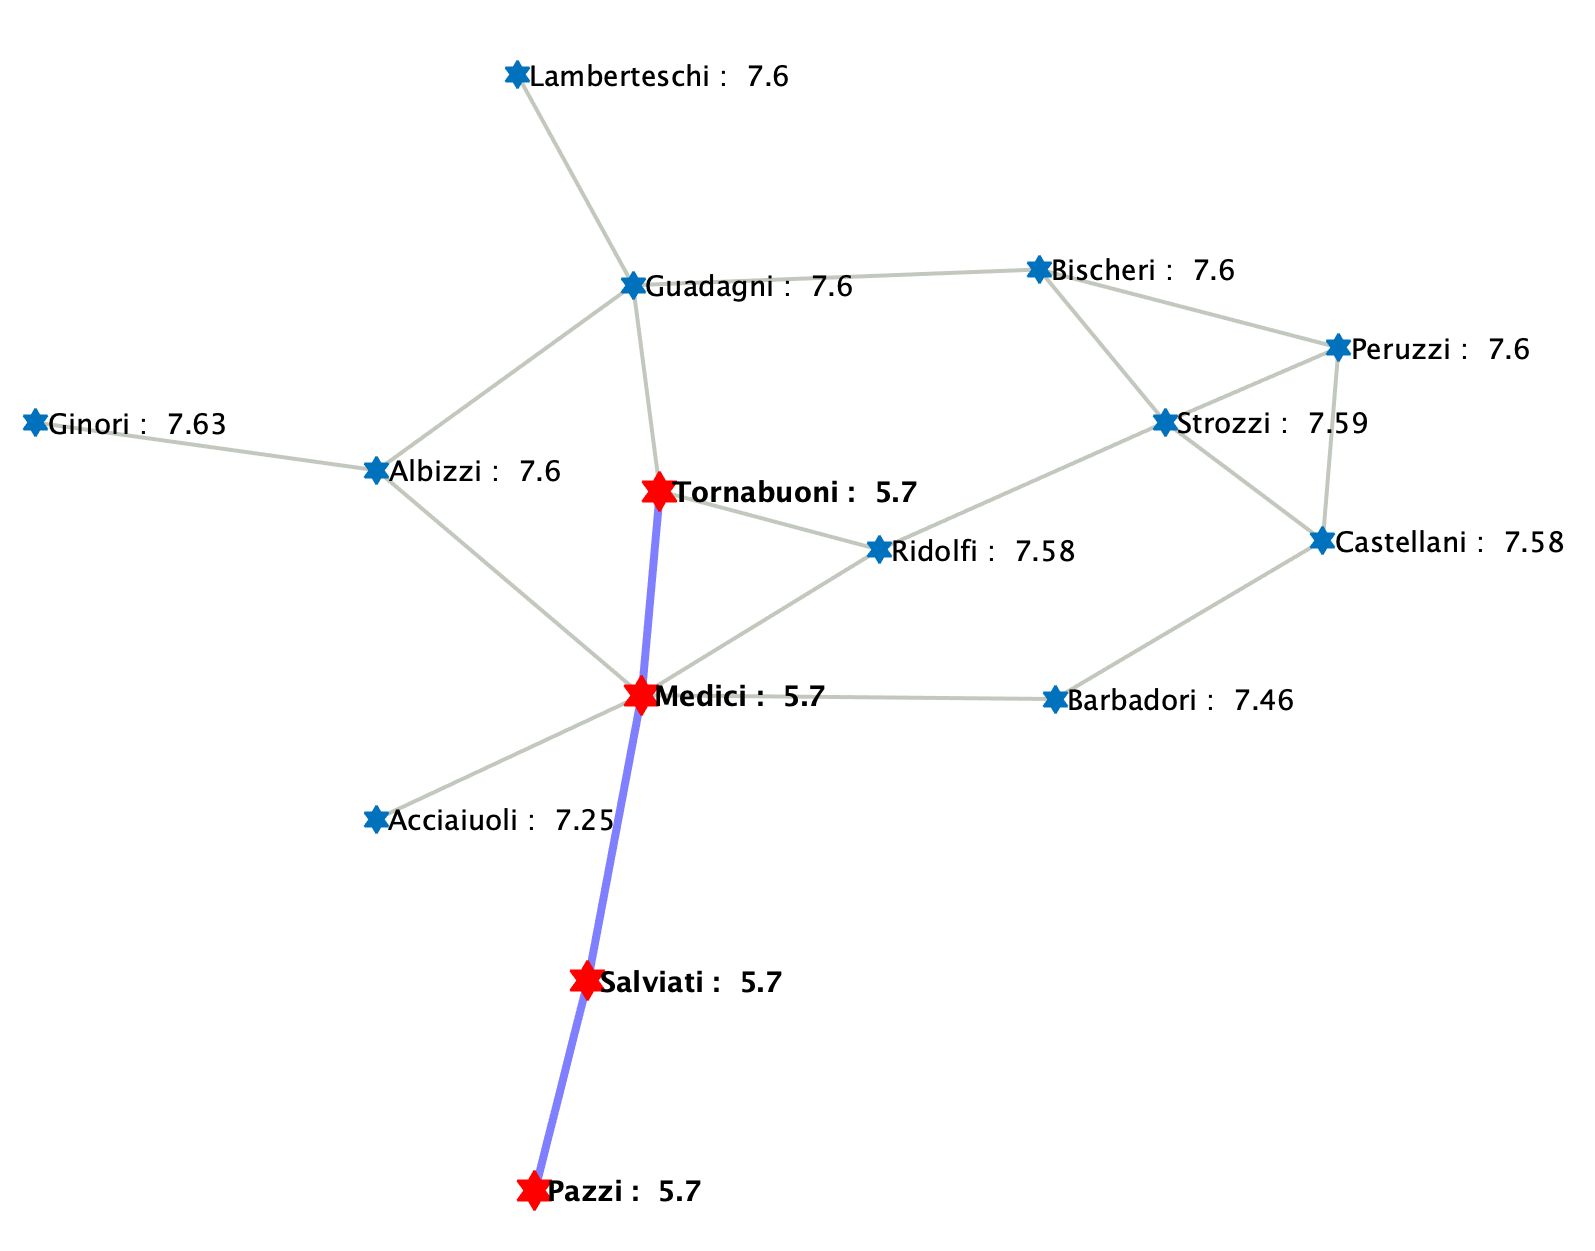
\includegraphics[scale=.18]{../Figures/introP45.png}
\end{frame}

\begin{frame}{Successful Quadruple-wise Updates}
\begin{overpic}[scale=.13]{../Figures/introP46.png}
\put(56,66){
\color{BrickRed}
(below roundoff)
}
\end{overpic}
\end{frame}

\begin{frame}{\small Consensus Error - Biased Quadruple-wise Updates}
\centering
    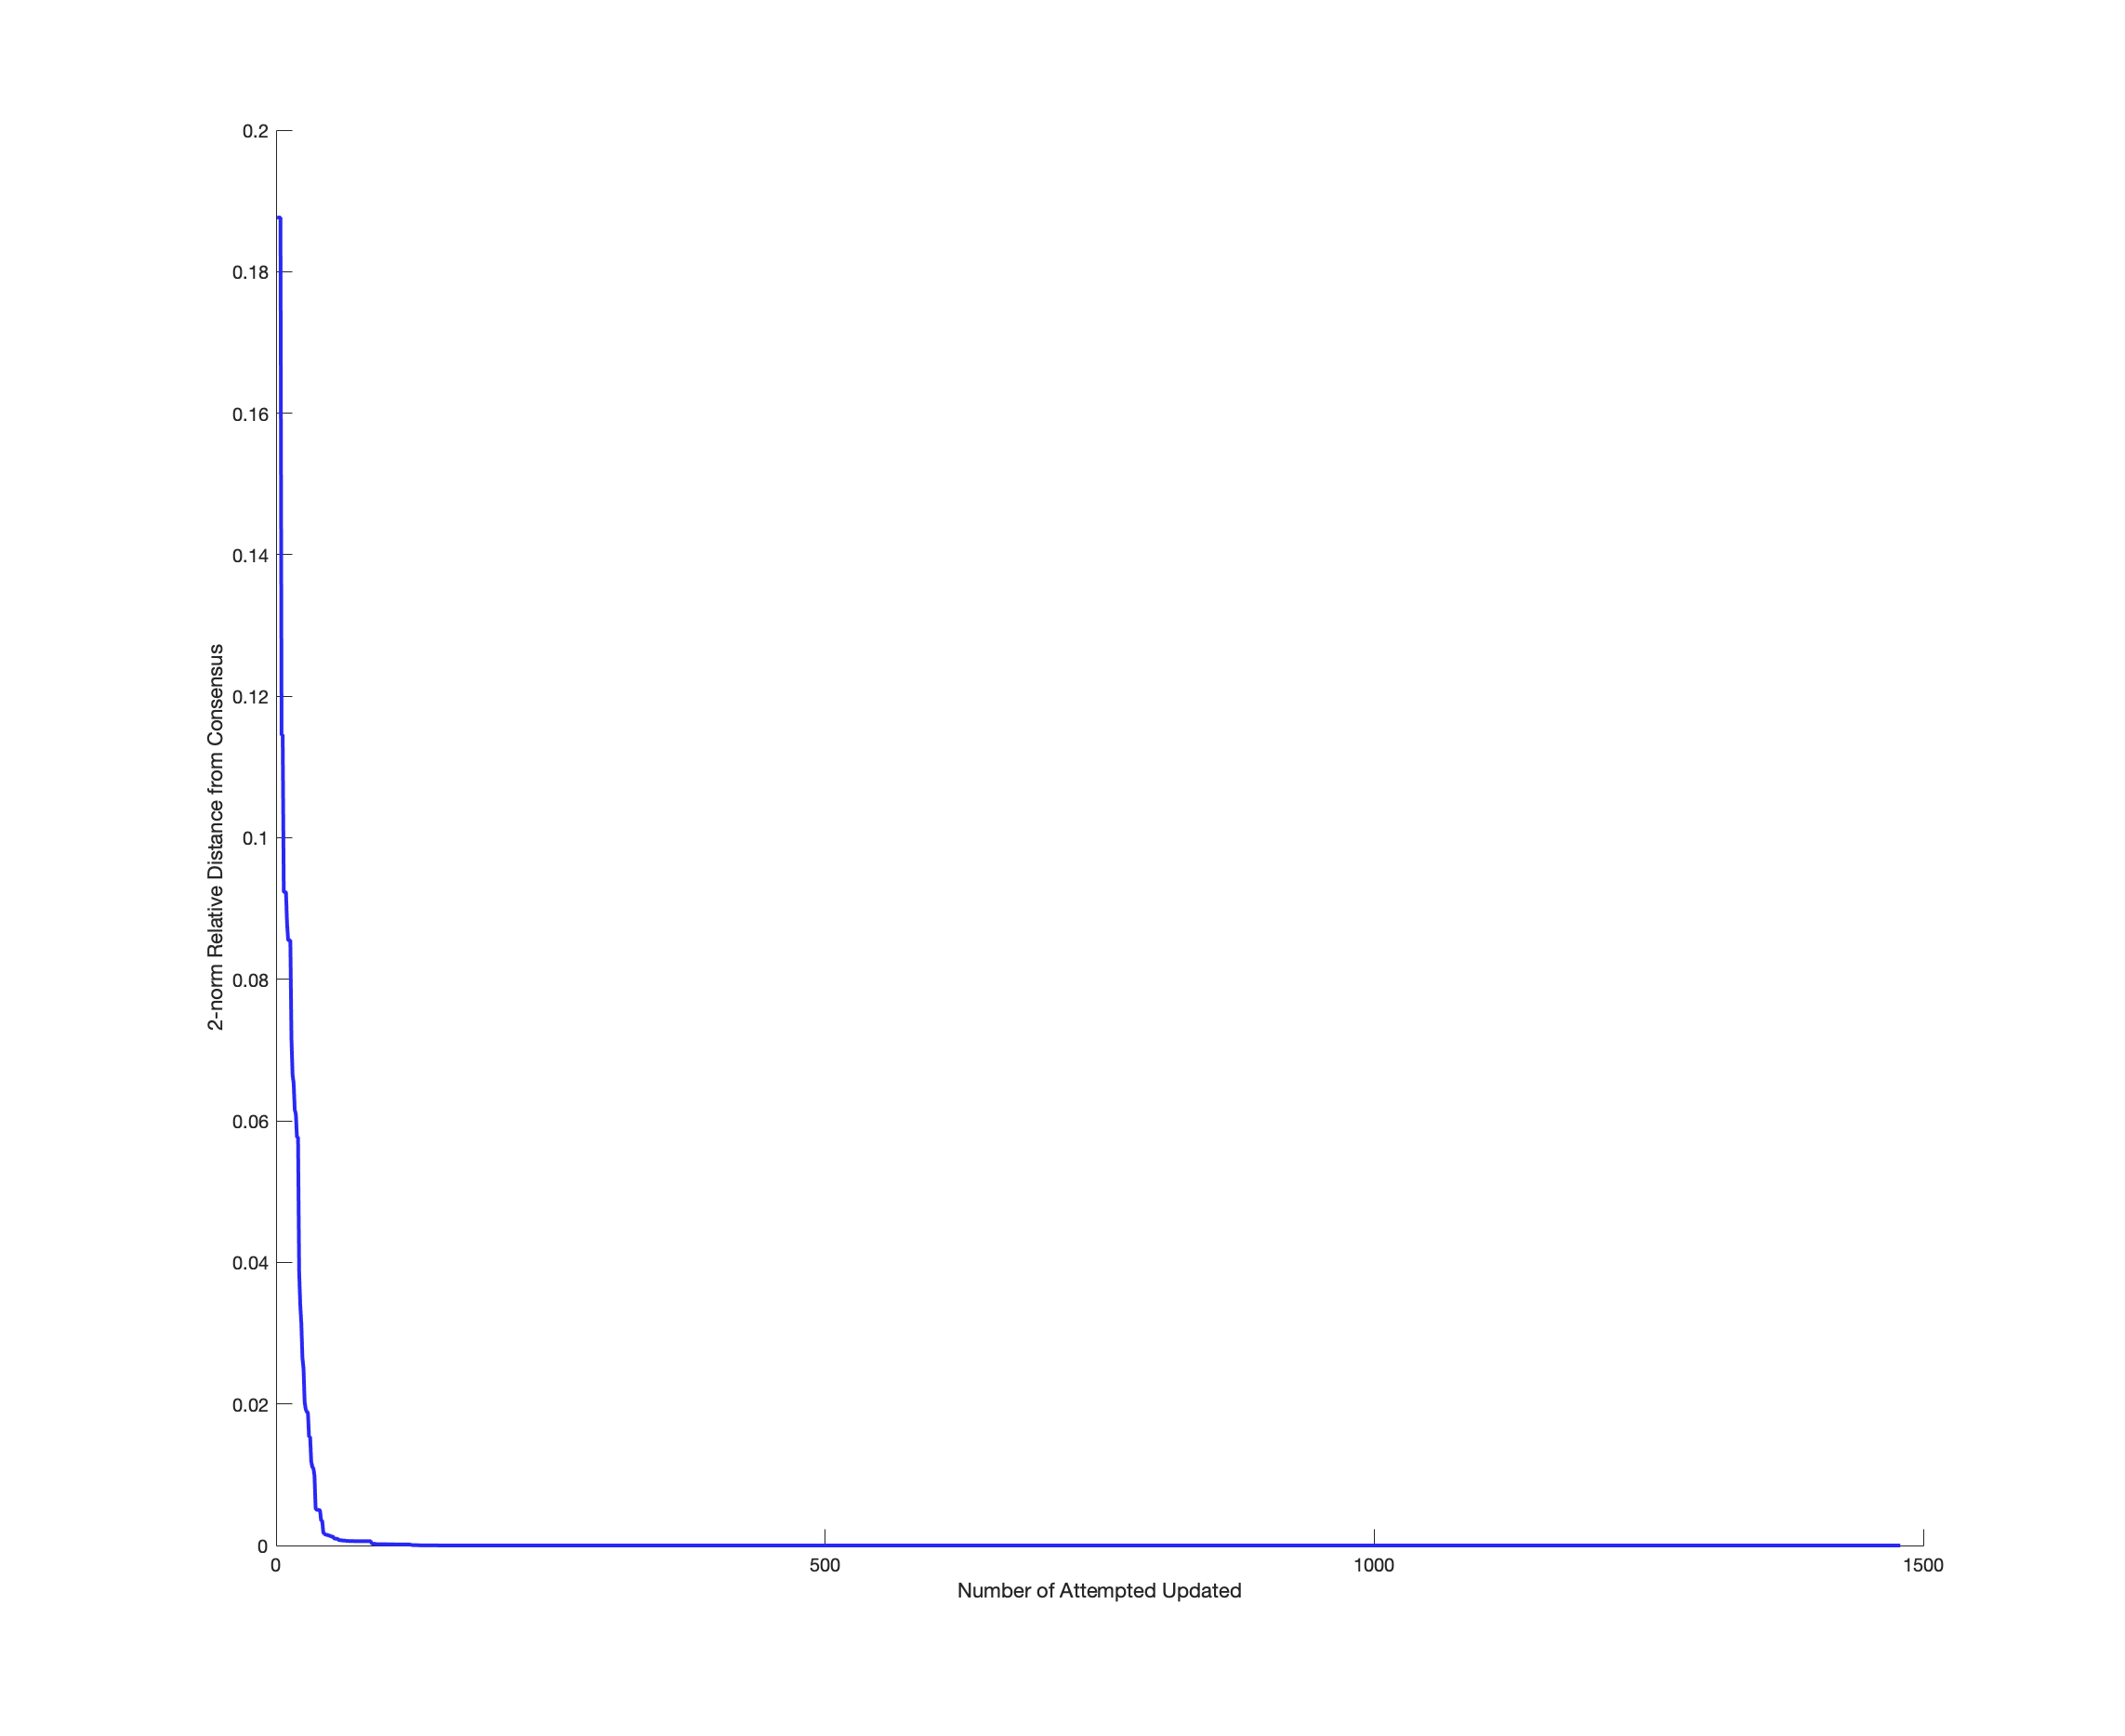
\includegraphics[scale=.13]{../Figures/introP47.png}
\end{frame}

\begin{frame}{\small Biased Quadruple-wise Updates - Steady state}
\centering
    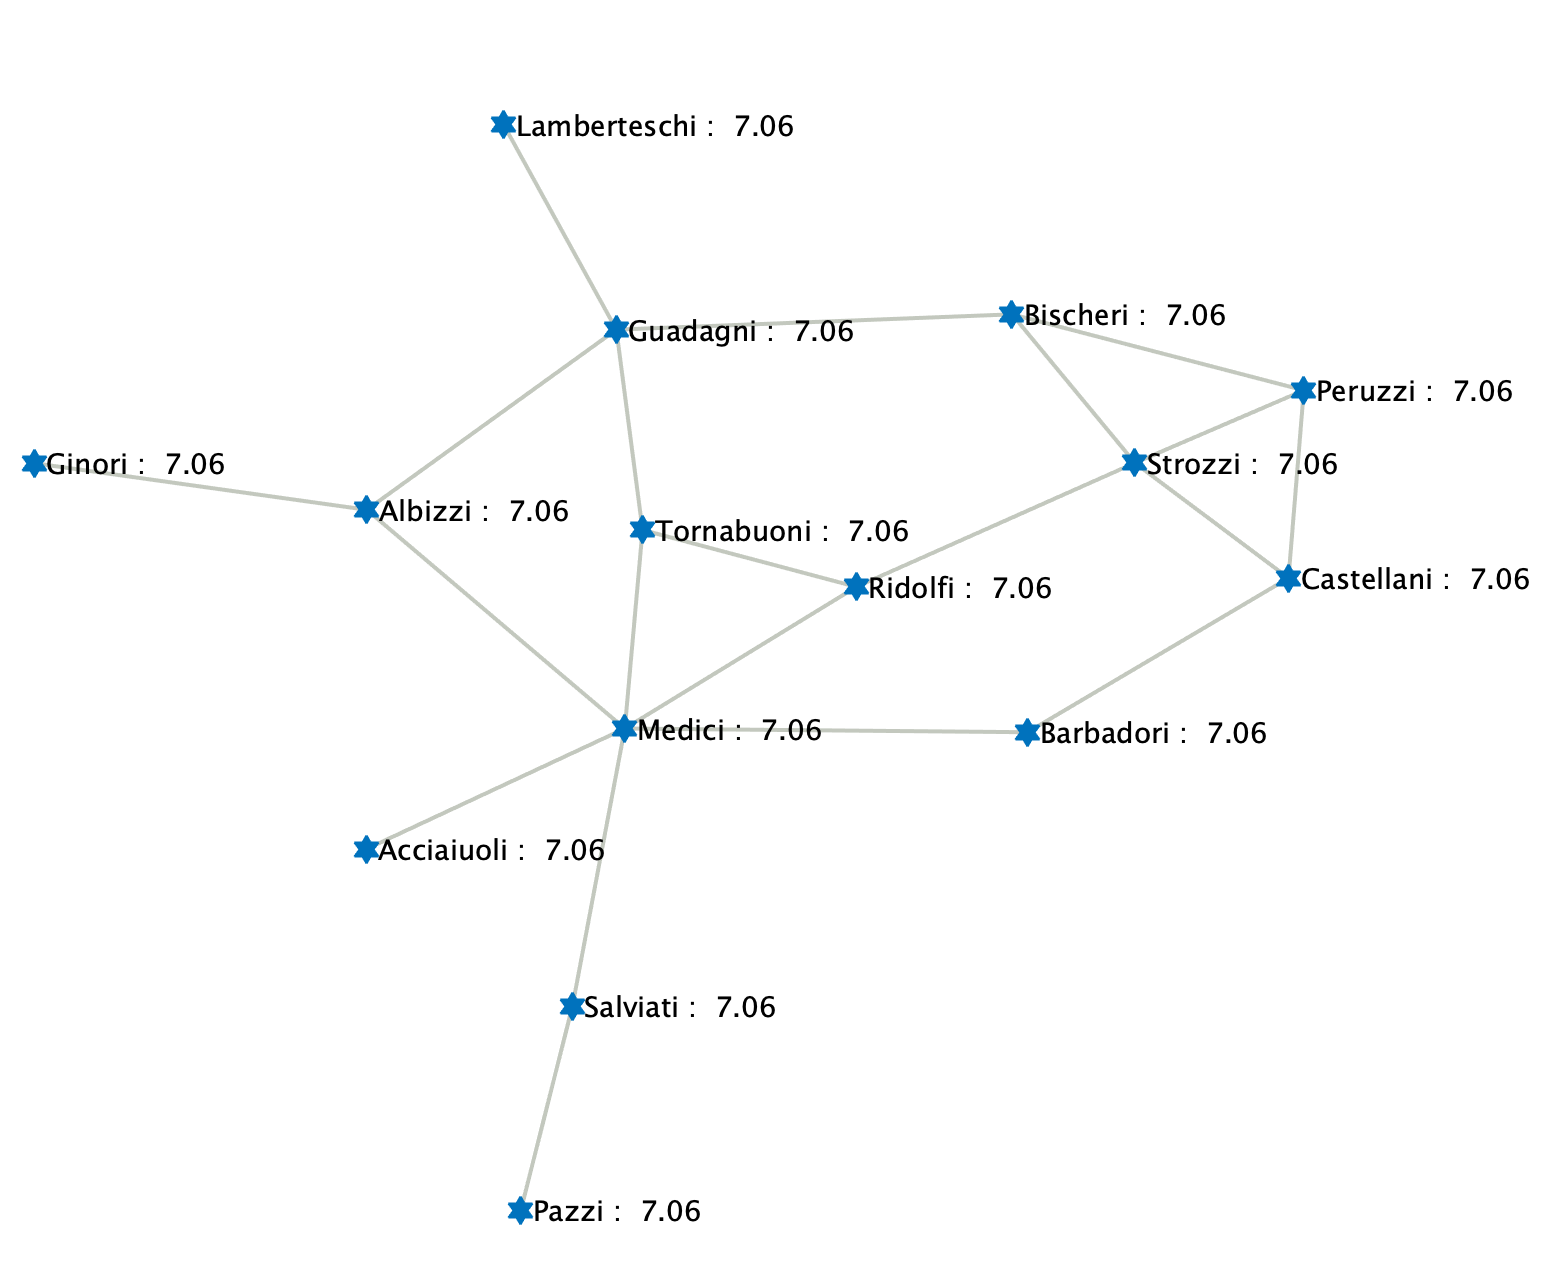
\includegraphics[scale=.18]{../Figures/introP48.png}
\end{frame}

\begin{frame}{Consensus Error - Biased $k$-group Updates}
\centering
    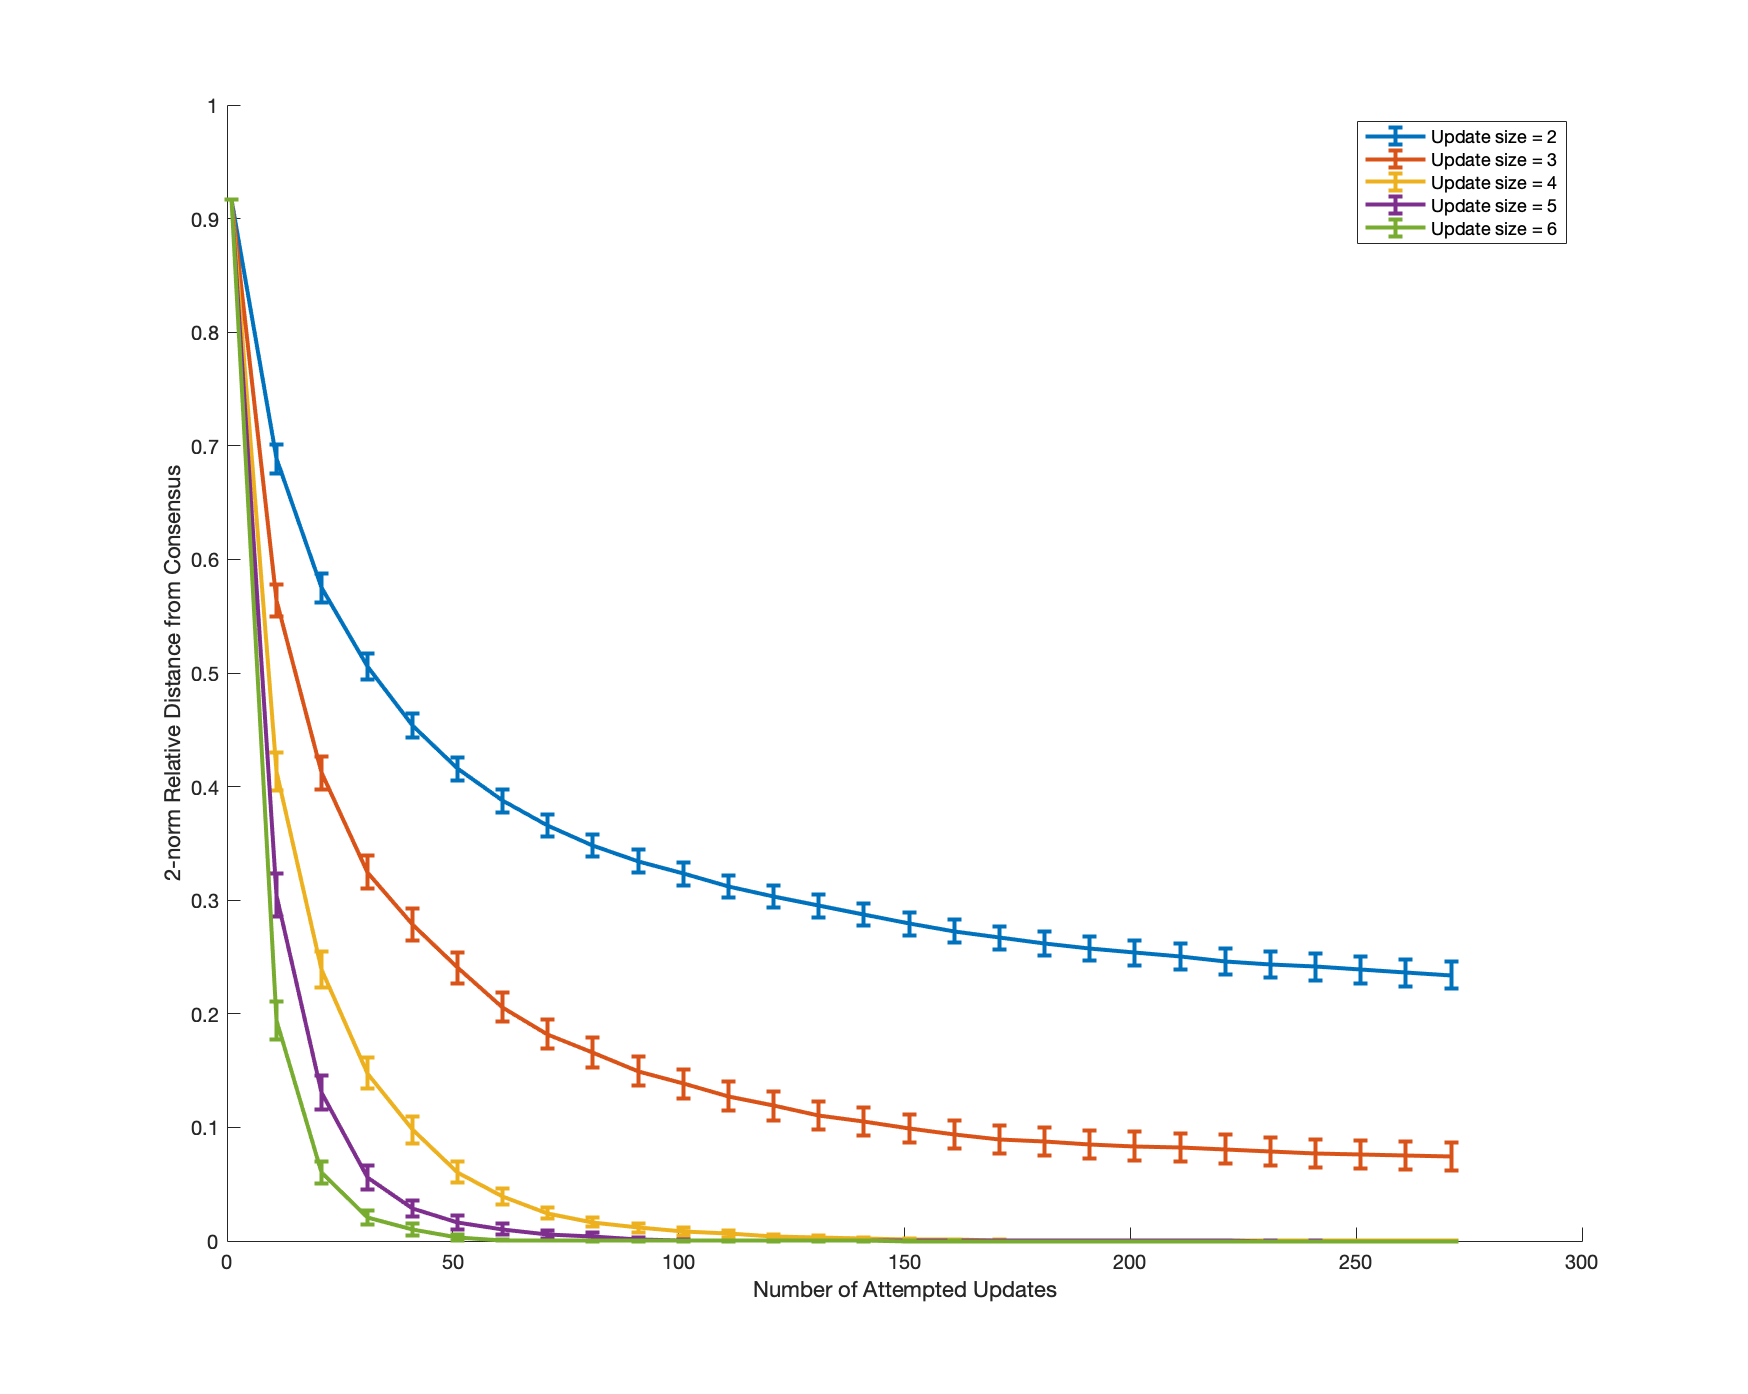
\includegraphics[scale=.175]{../Figures/errorBars.png}
\end{frame}

% Notes:
% Dataset of marriage relationships between 16 families in 15th
% century Florence.

% \begin{frame}{Introduction}
% \begin{figure}[!htb]
%     \centering
%     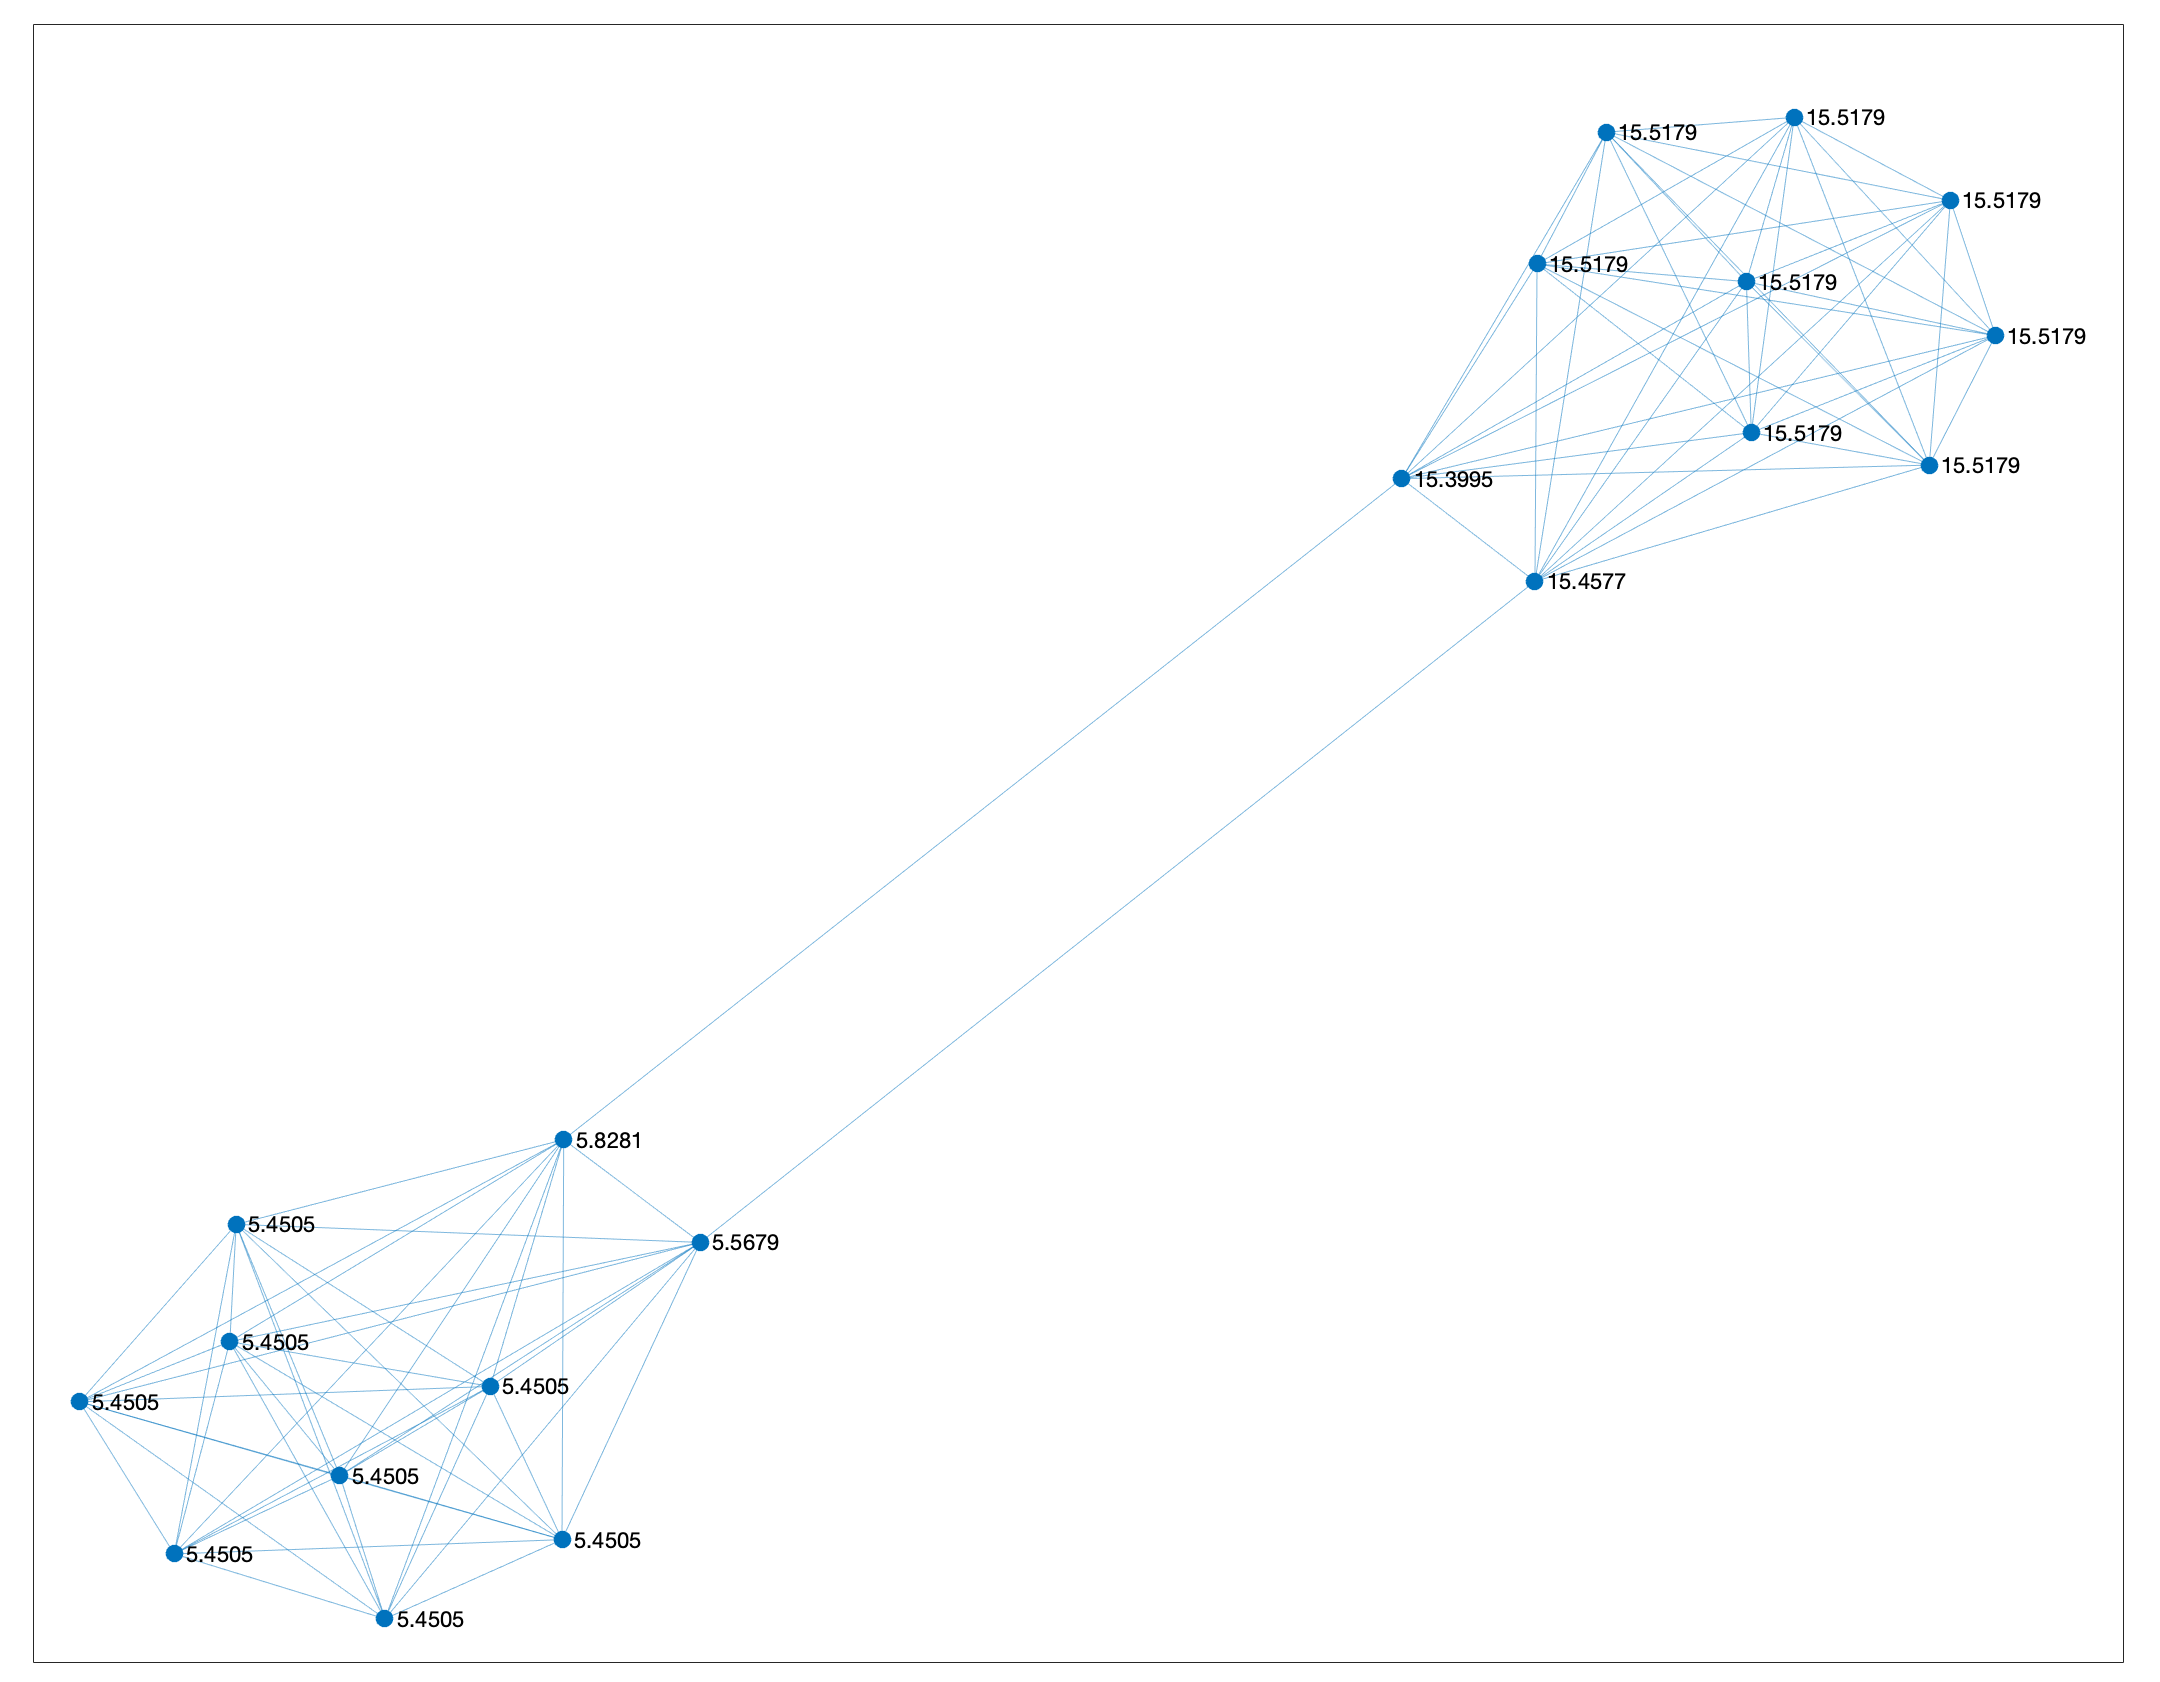
\includegraphics[scale=.24]{../Figures/deadlockedDoubleRoPk4.png}
%     \caption{Deadlocked configuration of opinions for updates of group size $4$.}
%     \label{fig:motivation1}
% \end{figure}
% \end{frame}

% \begin{frame}{Introduction}
% \begin{figure}[!htb]
%     \centering
%     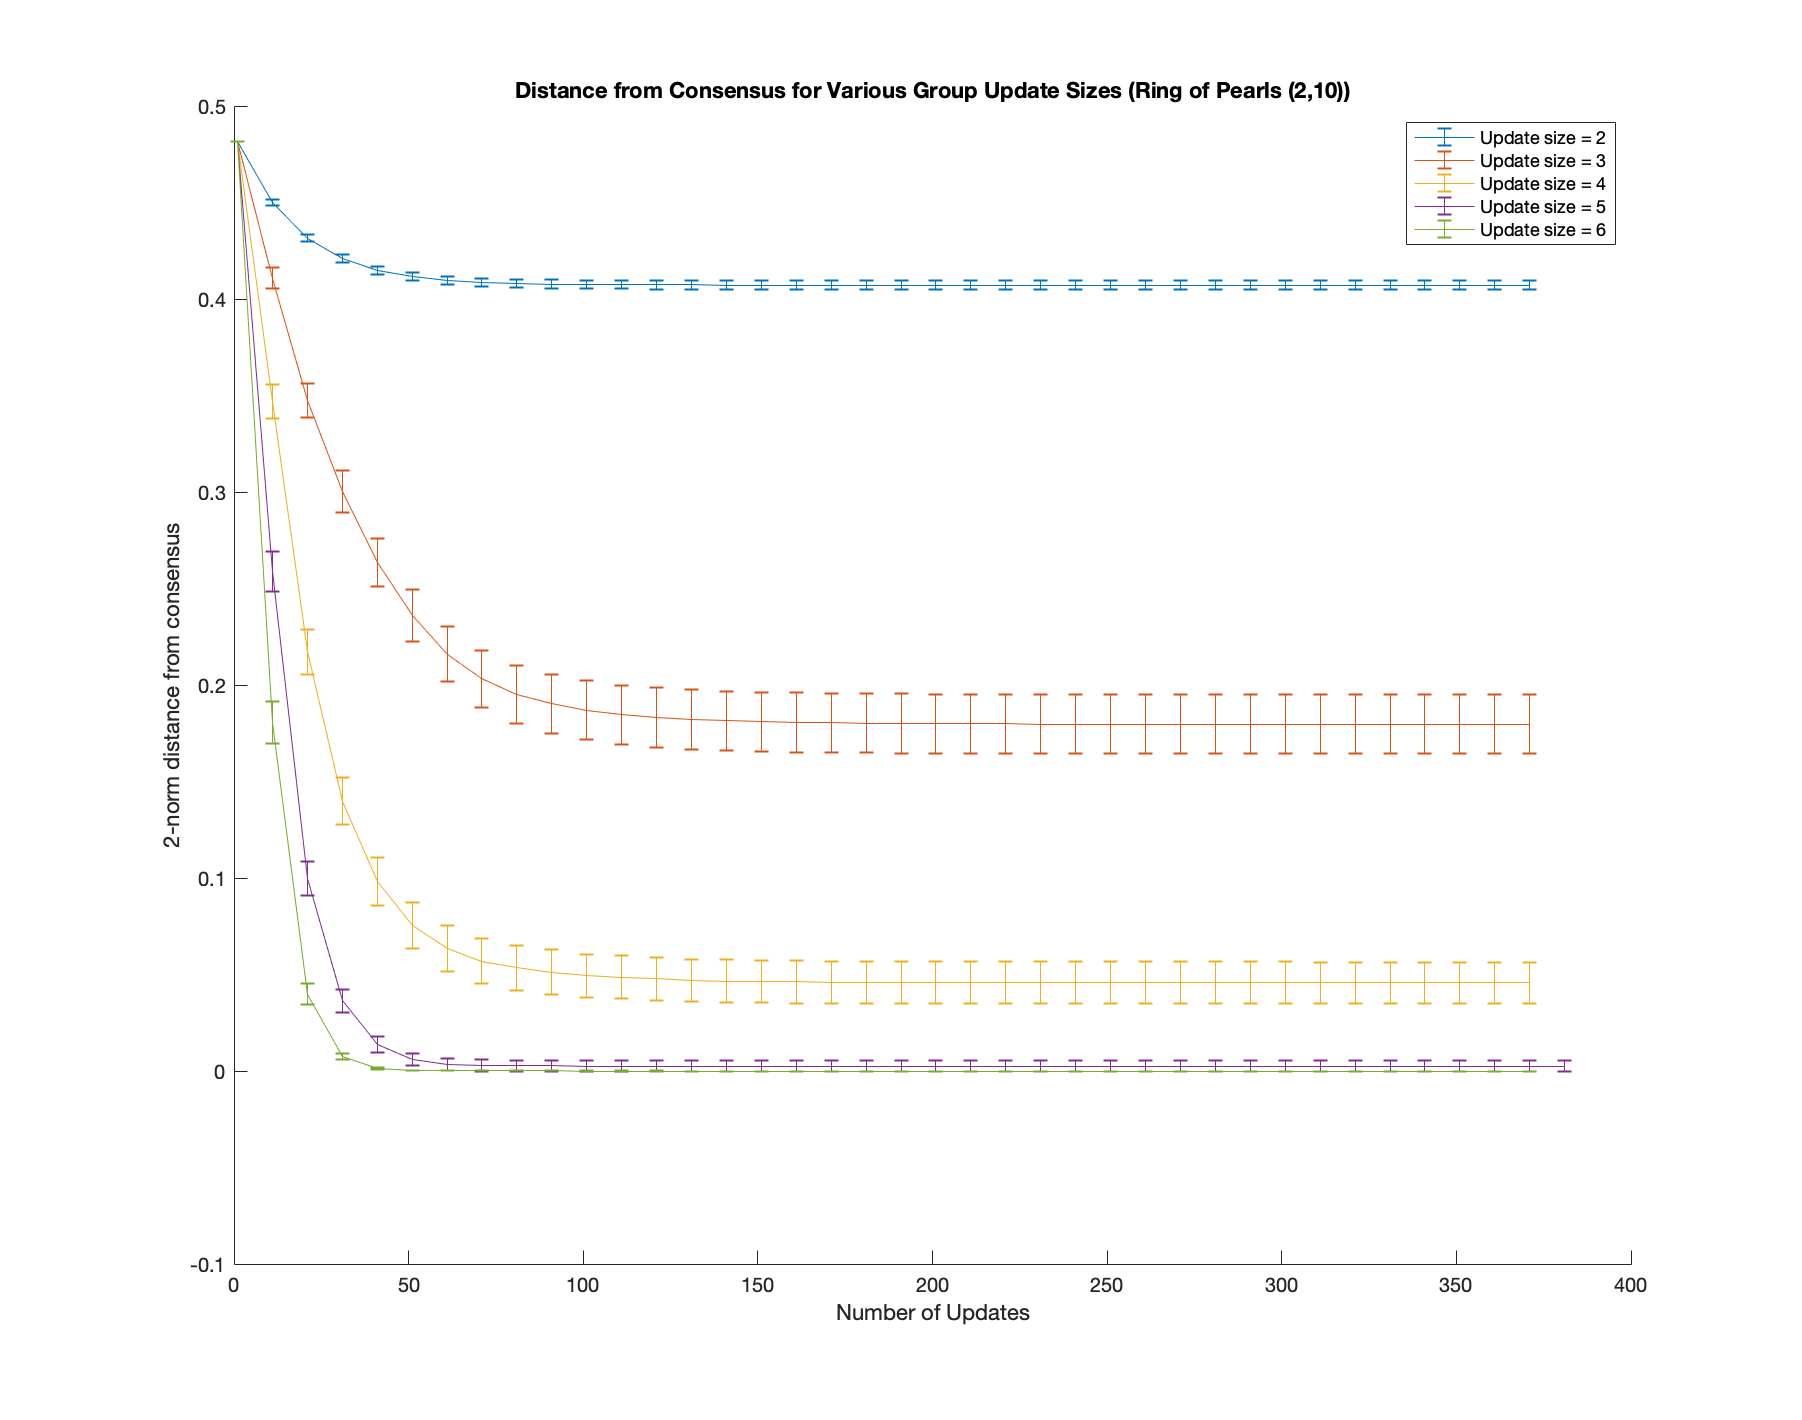
\includegraphics[scale=.13]{../Figures/RoP210ErrorBar.png}
%     \caption{Expectation and $.95$ confidence intervals for the distance from consensus of opinions for $500$ simulations. As group size of update increases, convergence to consensus becomes easier.}
%     \label{fig:motivation2}
% \end{figure}
% \end{frame}

\begin{frame}{Takeaways from Example}
	Observations:
	\begin{itemize}
		\item Conformity bias affects convergence and may stop it.
		\item Multi-scale updates may make convergence possible and accelerate convergence.
		\item Shared neighbors help updates; opinions of unshared neighbors will determine feasibility of update.
	\end{itemize}
	\pause
	$$
\Downarrow
	$$
	\pause
	Factors to consider:
	\begin{enumerate}
		\item Network structure
		\item Multi-scale communication
		\item Biases
	\end{enumerate}
\end{frame}

\begin{frame}{Overview}
\tableofcontents
\end{frame}

\section{Rate of Convergence for Unbiased Multi-scale Consensus}

\begin{frame}{Unbiased Multi-scale Update Rule}
\begin{itemize}
    \item Multi-scale updates: Communication occurs between pairs of individuals and/or among individuals within groups of various sizes.
	    \pause
    \item Parital consensus: when a connected group of individuals $S$ of size $M$ communicates at timestep $k$, they update their opinions by a fraction $0<\beta\leq1$ to the group average:
    \begin{equation}{\label{eq:updateRule}}
        x_i(k+1) = (1-\beta)x_i(k) + \beta\frac{\sum_{j\in S}x_j(k)}{M}, \; i\in S.
    \end{equation}
    \pause
    \item We have derived lower bounds and upper bounds on the \textit{expected} convergence rates to consensus: they depend on 1. group sizes, 2. network topology, 3. partial consensus size $\beta$, and 4. communication rates of individuals/groups.
\end{itemize}
\end{frame}

\begin{frame}{Convergence Results}
	    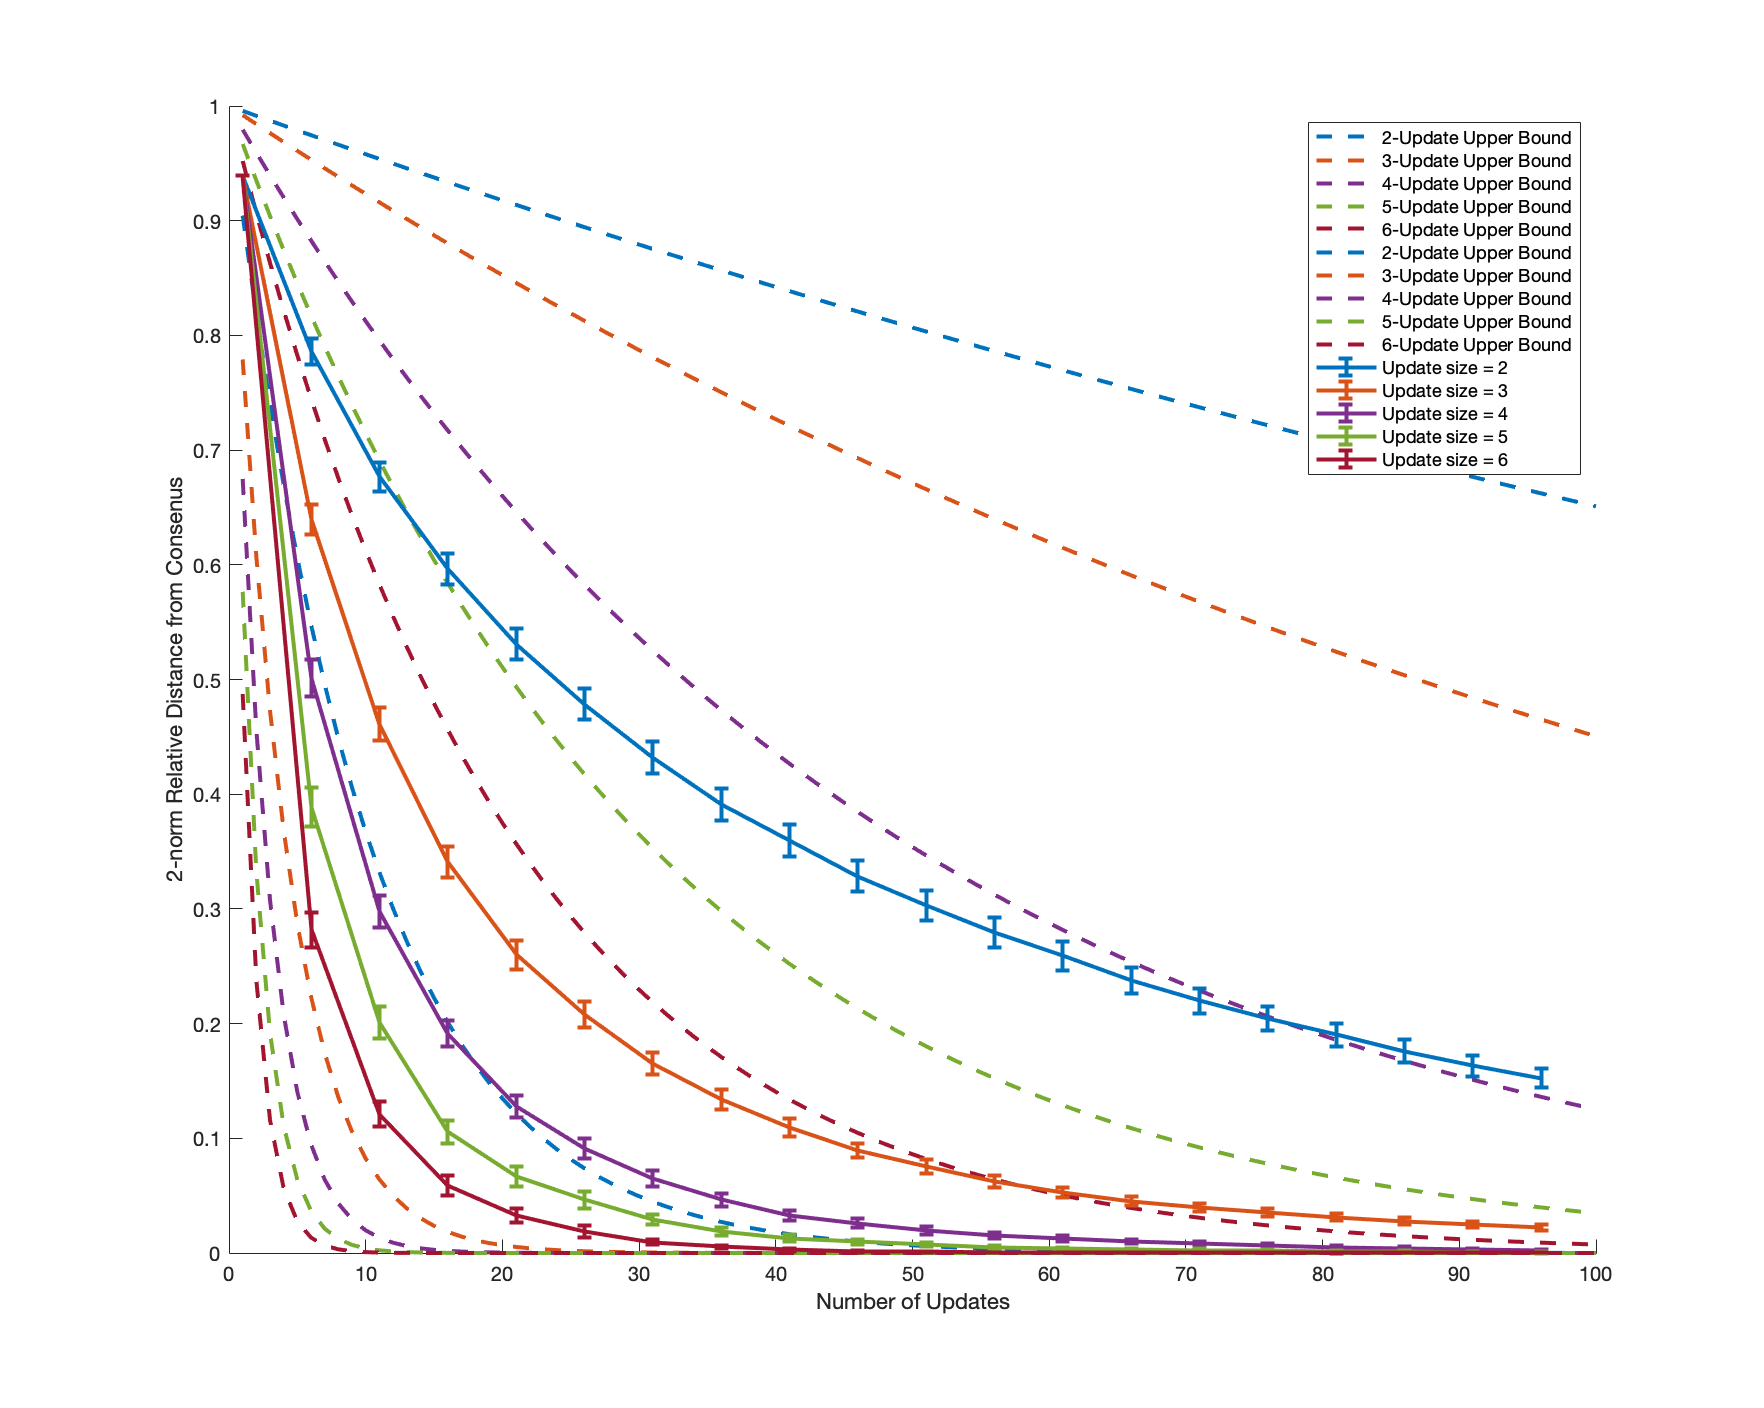
\includegraphics[scale=.17]{../Figures/noBiasConvergenceErrorBounds.png}
\end{frame}

\section{Rate of Convergence of Biased Partial Consensus}

\begin{frame}{Conformity Bias}
\begin{itemize}
    \item Upon communication, a pair of individuals updates their opinions as
    \begin{equation}{\label{eq:updateRule}}
        x_i(k+1) = (1-\beta)x_i(k) + \beta\frac{x_i(k)+x_j(k)}{2}
    \end{equation}
    \pause
    \item Assume individuals have a \textit{conformity bias}: in a graph $G$ of size $n$ with adjacency matrix $A$, a group $S$ of size $M$ will update at timestep $k$ only if
    \begin{equation}{\label{eq:biasRule}}
        \sum_{i\in S}\sum_{j=1}^nA_{ij}(x_i(k+1)-x_j(k+1))^2-\sum_{i\in S}\sum_{j=1}^nA_{ij}(x_i(k)-x_j(k))^2 < 0
    \end{equation}
\end{itemize}
\end{frame}

\begin{frame}{Biased Pairwise Partial Consensus}
    \begin{proposition}[partial consensus is possible somewhere] {\label{prop:updatePairExistence}}
	For any graph $G$ of $m$ edges and any vector $x\in\R^n$ of values indexed by the nodes of $G$, there exists a pair of adjacent nodes $p,q\in\mathcal{V}(G)$ and a $\beta\geq1/2m$ such that an update under conformity bias is possible between nodes $p$ and $q$.
\end{proposition}
\pause
\begin{theorem}[$\implies$ convergence to consensus]{\label{theorem:betaConvergence}}
	Assume that at each timestep $k$, the pair of nodes $p,q\in\mathcal{V}(G)$ with the largest possible conformity biased update $\beta_k|x_{p_k}(k)-x_{q_k}(k)|$ are updated. Denote $L$ the graph Laplacian of the graph $G$, $\lambda_2(L)$ the second smallest eigenvalue of $L$, and $x_\text{ave}$ the average opinion. Then, for all $k$, 
	$$
	\beta_k|x_{p_k}(k)-x_{q_k}(k)|\geq\frac{\lambda_2(L)^{1/2}}{\sqrt{2}nm^{3/2}}\|x-x_{\text{ave}}\|_2.
	$$
\end{theorem}
\end{frame}

\section{Deadlock Formation under Biased Full Consensus}

\begin{frame}{Biased Full Consensus}
\begin{itemize}
    \item Groups of individuals update to \textit{full} consensus:
    \begin{equation}{\label{eq:updateRuleFull}}
        x_i(k+1) = \frac{\sum_{j\in S}x_j(k)}{M}, \; i\in S.
    \end{equation}
    \pause
    \item Individuals have conformity bias:
    \begin{equation*}
        \sum_{i\in S}\sum_{j=1}^nA_{ij}(x_i(k+1)-x_j(k+1))^2-\sum_{i\in S}\sum_{j=1}^nA_{ij}(x_i(k)-x_j(k))^2 < 0
    \end{equation*}
    \pause
    \item Opinion deadlocks at various scales form in some graphs.
	    \pause
    \item Multi-scale updates break opinion deadlocks in various graphs.
	    \pause
    \item Main thrust: classification
\end{itemize}
\end{frame}

\begin{frame}{Pairwise Opinion Deadlocked Graphs}
    Graphs that can become pairwise deadlocked:
    \begin{itemize}
        \item Cycle Graphs of $n\geq 9$ nodes.
        \item Star Graphs of $n\geq5$ leaf nodes.
        \item Path Graphs of $n\geq5$ nodes.
        \item Padgett's Florentine Families Network.
    \end{itemize}
\end{frame}

\begin{frame}{Pairwise Opinion Deadlocked Graphs}
    \begin{figure}[!htb]
    \centering
    \begin{subfigure}{.49\textwidth}
        \centering
    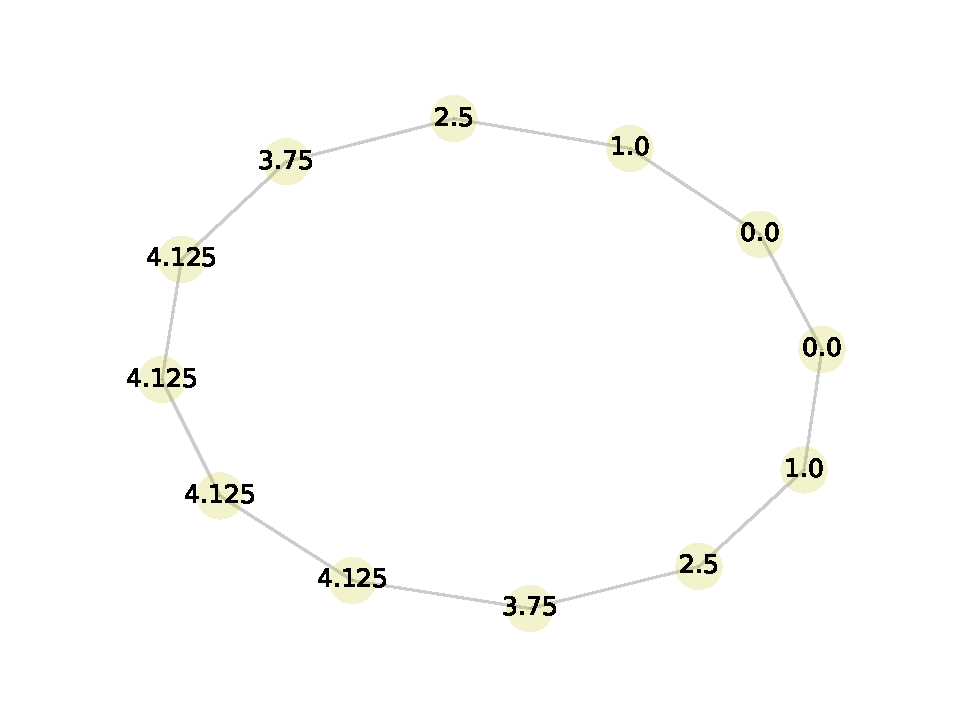
\includegraphics[scale=.3]{../Figures/success_graph_with_12_nodes_code_9.pdf}
    \subcaption{Deadlocked cycle graph of $12$ nodes.}
    \label{fig:deadlockedCycle}
    \end{subfigure}
    \begin{subfigure}{.49\textwidth}
        \centering
    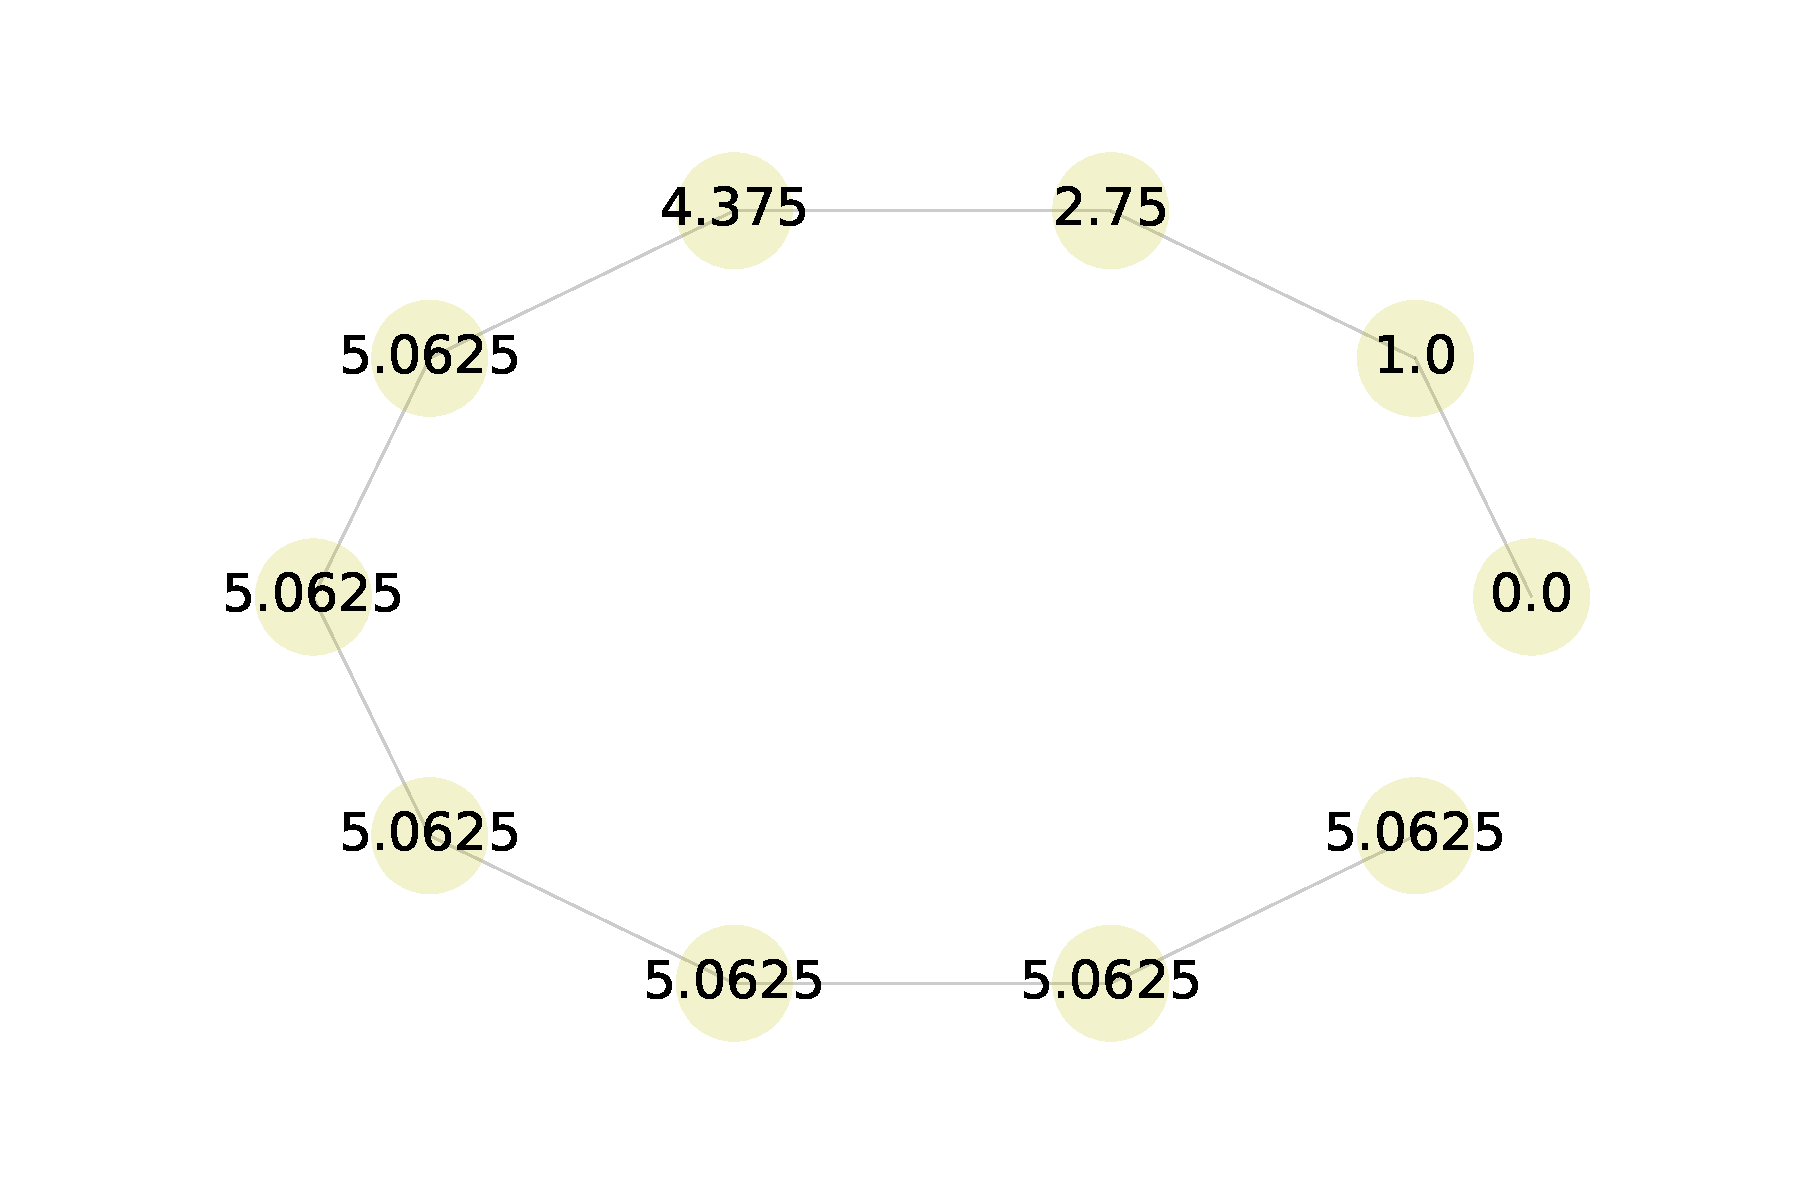
\includegraphics[scale=.18]{../Figures/success_graph_with_10_nodes_code_path_10.pdf}
    \subcaption{Deadlocked path graph of $10$ nodes.}
    \label{fig:deadlockedPath}
    \end{subfigure}
    \caption{Examples of pairwise deadlocked graphs.}
\end{figure}
\end{frame}

%\begin{frame}{Pairwise Opinion Deadlocked Graphs}
%    \begin{figure}[!htb]
%        \centering
%    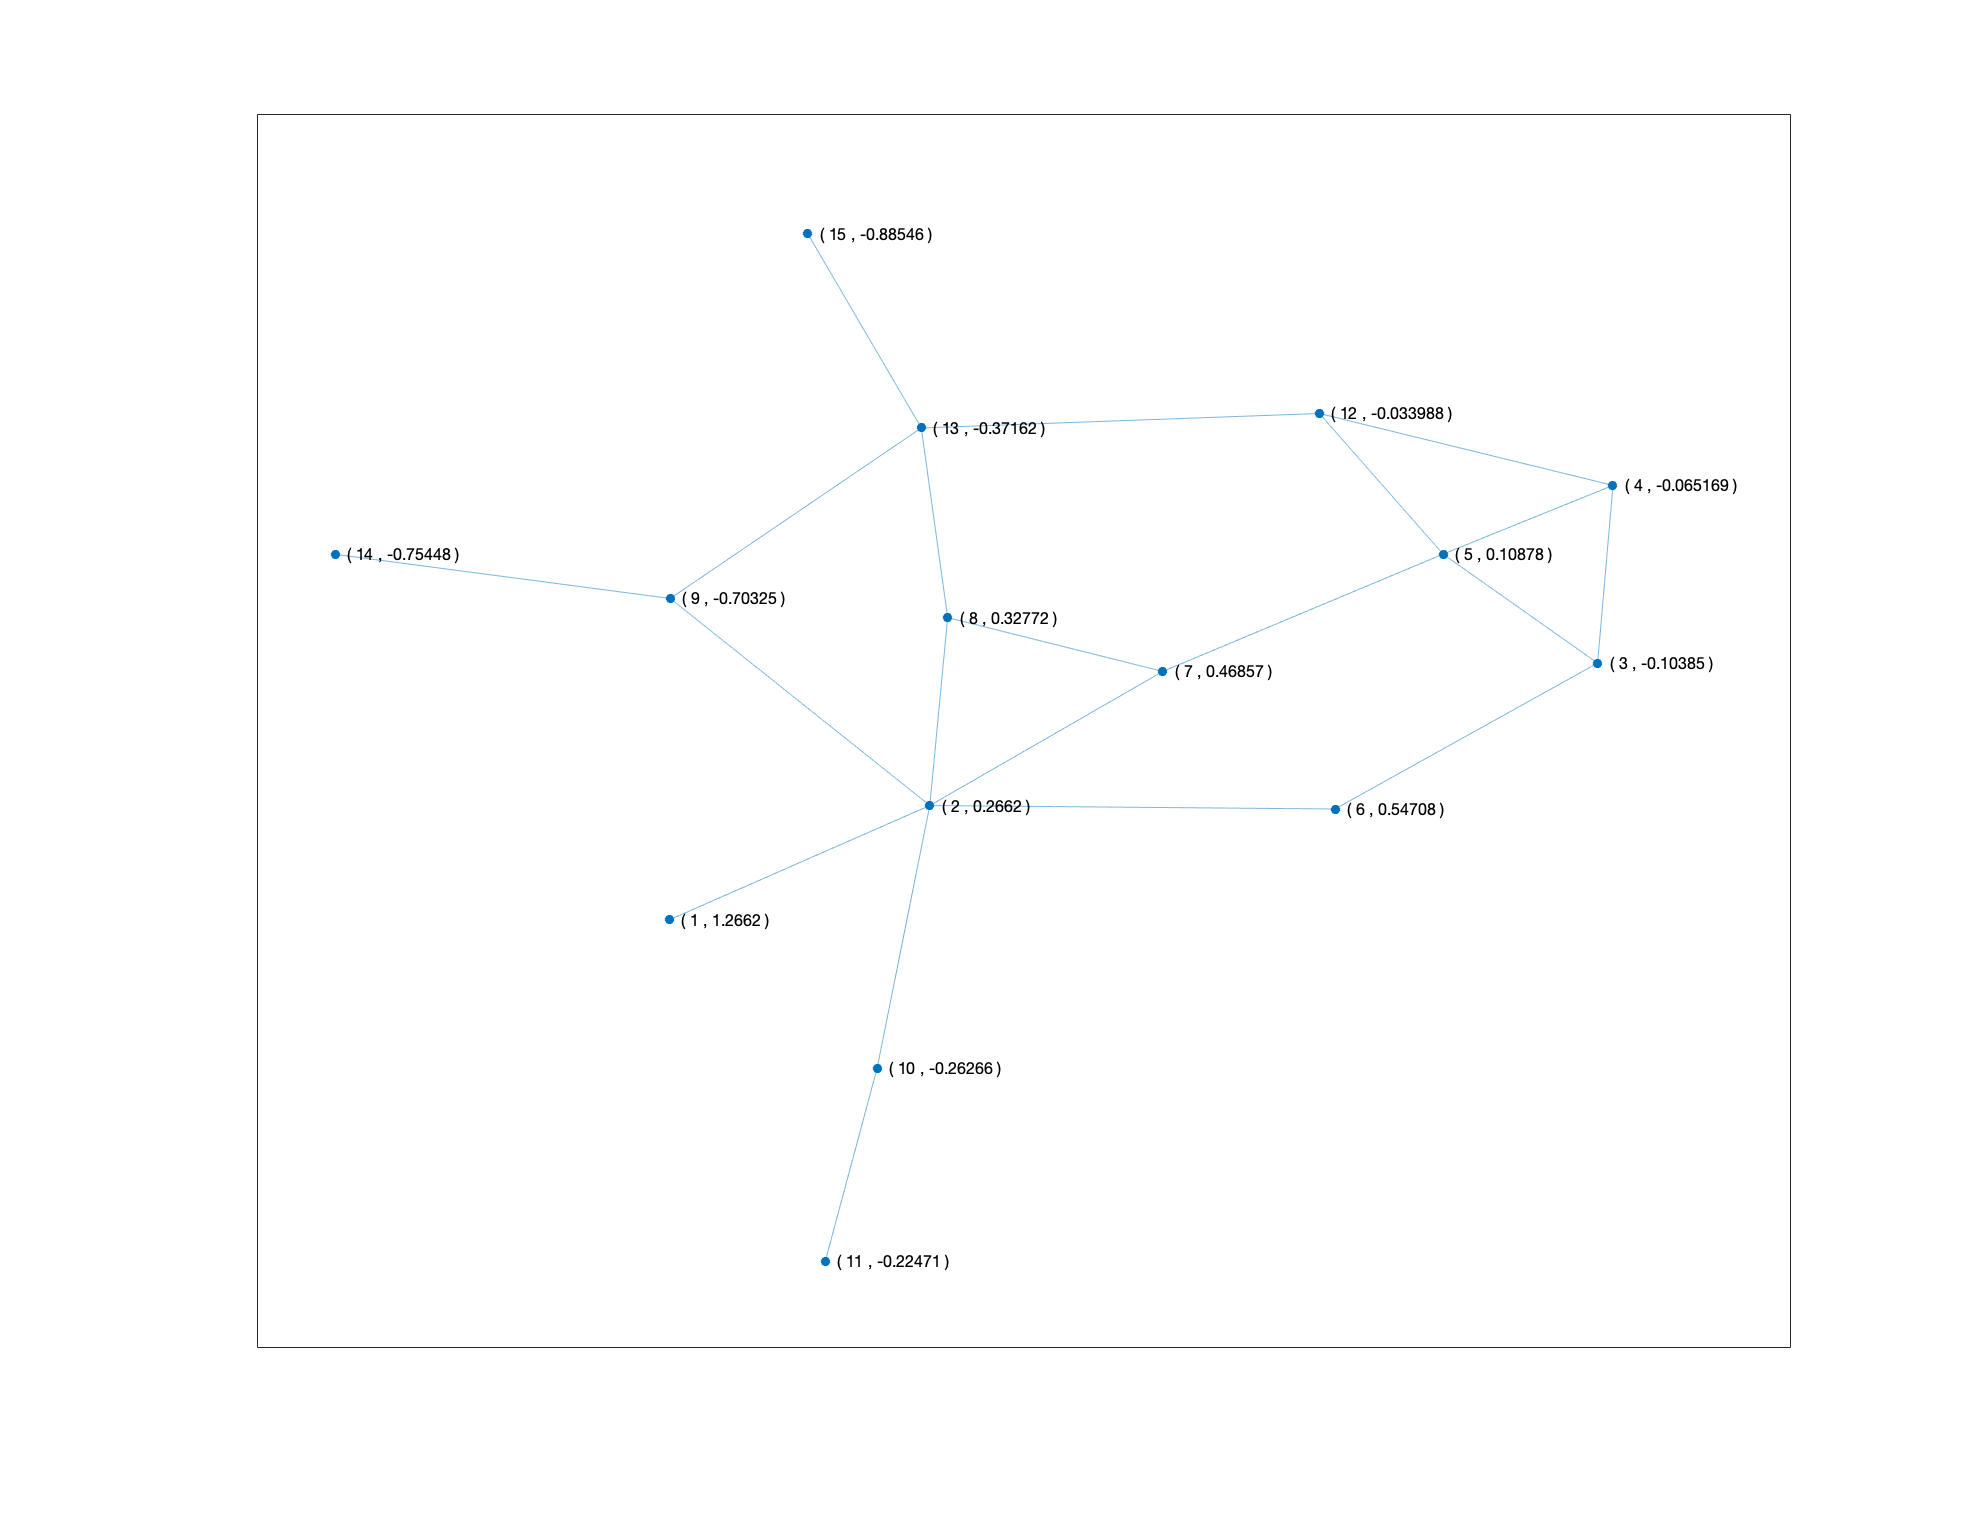
\includegraphics[scale=.13]{../Figures/florentine.png}
%        \label{fig:deadlockedFlorentine}
%        \caption{Deadlock in the Padgett's Florentine Families Network}
%    \end{figure}
%\end{frame}

\begin{frame}{Graphs Immune to Pairwise Deadlock}
\begin{itemize}
    \item Complete Graphs
    \item Erdos-Renyi Graphs $G(N,p)$ with sufficiently high $p$ seem to have a low probability of becoming deadlocked.
\end{itemize}
\begin{figure}[!htb]
    \centering
    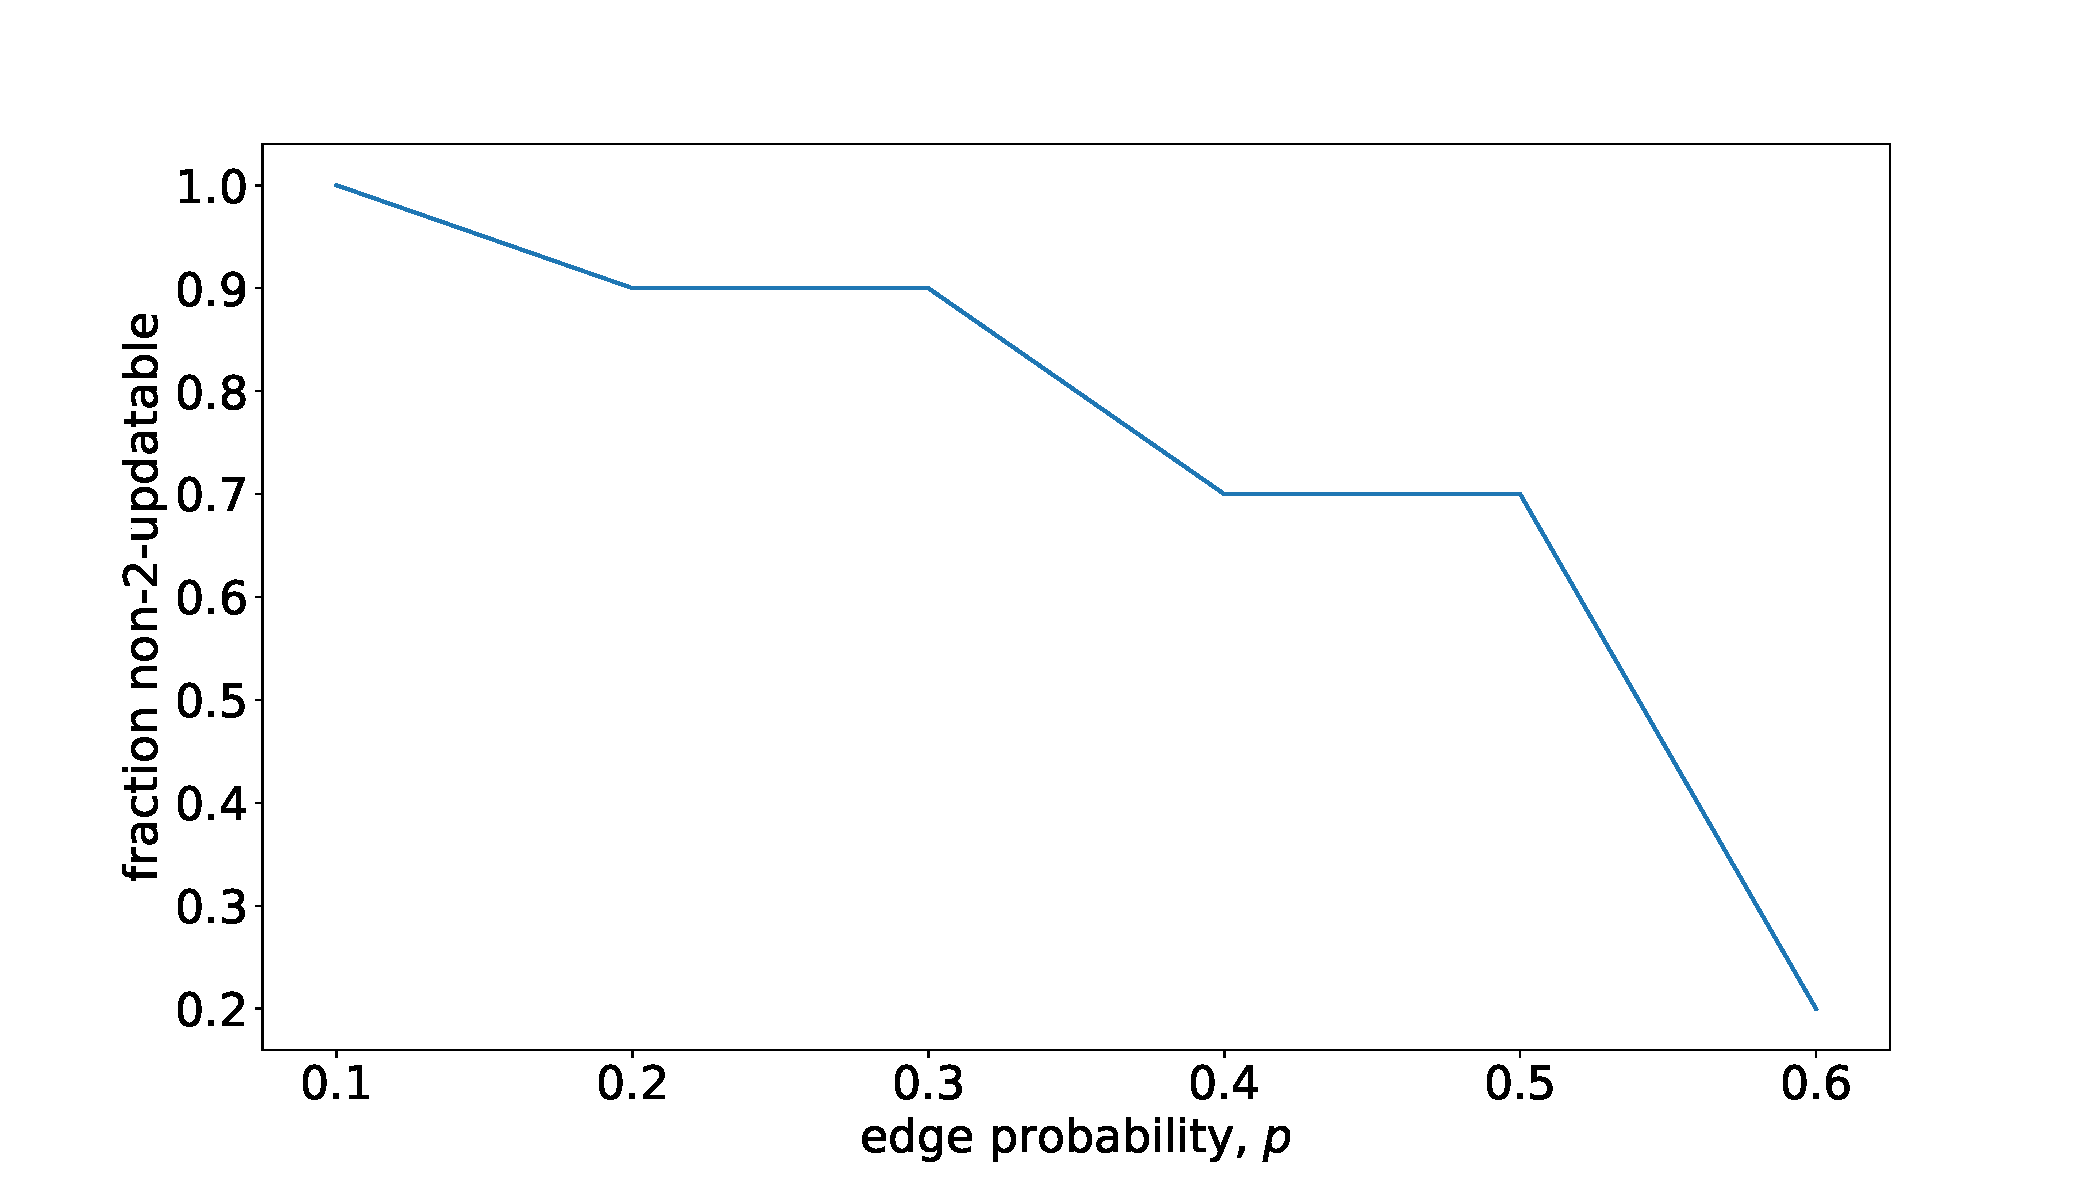
\includegraphics[scale=.2]{../Figures/compare_ER_7_nodes_0_1-0_9_10_trials.pdf}
    \caption{Probability of immunity to deadlock of $G(N,p)$ increases with $p$.}
    \label{fig:erdosRenyiDeadlocked}
\end{figure}
\end{frame}

\begin{frame}{Multi-scale Opinion Deadlocked Graphs}
\begin{itemize}
    \item Star graphs of $5\leq n \leq 8$ nodes can become pairwise deadlocked but not triad deadlocked.
    \item Dumbbell graphs of $n\geq 10$ nodes can become deadlocked for all group sizes less than $n$.
\end{itemize}
\begin{figure}[!htb]
    \centering
    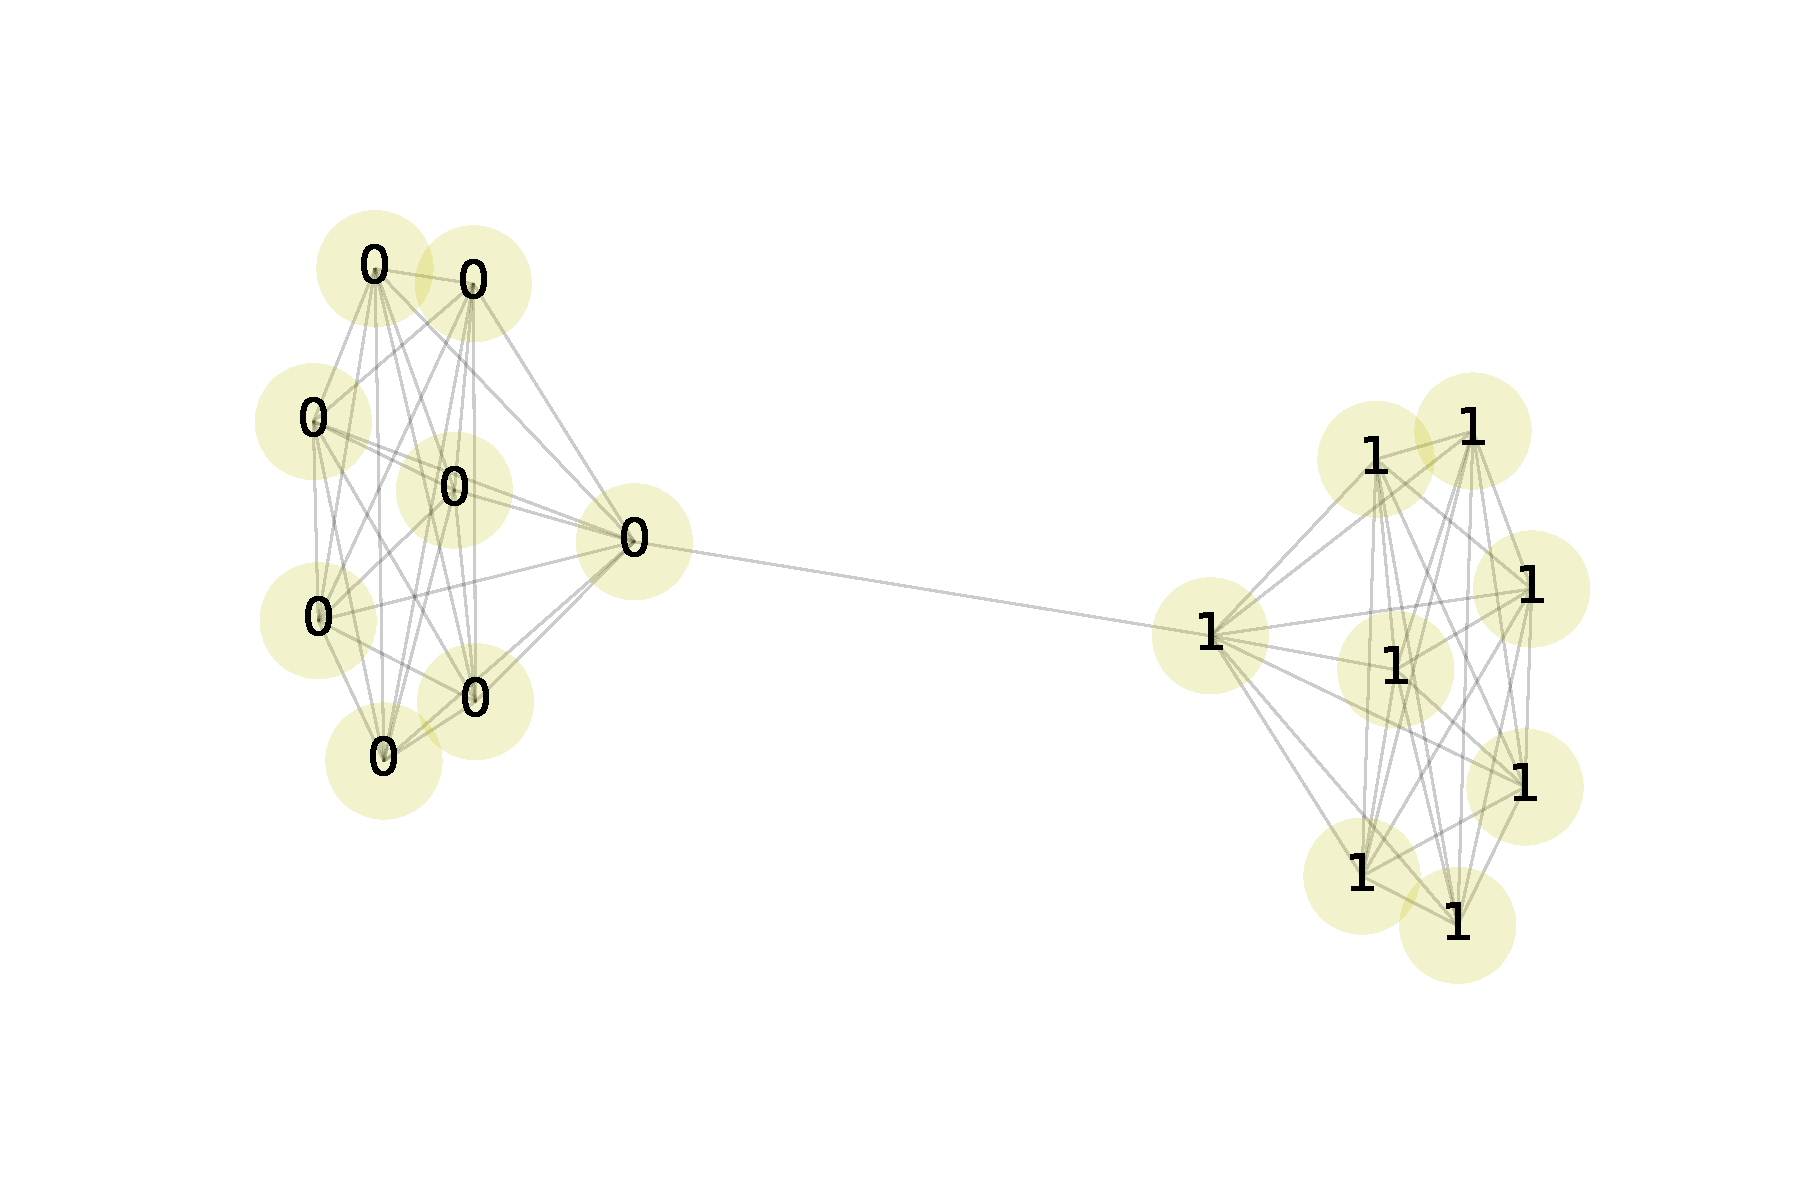
\includegraphics[scale=0.22]{../Figures/barbell.pdf}
    \caption{Deadlocked barbell graph of $n=16$ nodes.}
    \label{fig:deadlockedBarbell}
\end{figure}
\end{frame}

\begin{frame}{}
\centering
    MURI N00014-17-S-F006
    \vfill
    Thank you.
\end{frame}

% \begin{frame}{Introduction}
% \begin{itemize}
%     \item Opinion dynamics in a social network is a complicated process depending on:
%     \begin{enumerate}
%         \item The structure of the social network.
%         \item The frequency and nature of communication.
%         \item Individual biases.
%     \end{enumerate}
%     \item Understanding how opinions depend on 1-3 will inform the applications of interventions to encourage agreement, e.g.:
%     \begin{itemize}
%         \item Modify the structure of an opinion-deadlocked network.
%         \item Modify communication frequency or enable multi-scale/group communication via technology, scheduled meetings, etc.
%         \item Modify individual biases via, e.g., educational strategies.
%     \end{itemize}
% \end{itemize}
% \end{frame}

% %%%%% YK: I use the word configuration below to refer to the value of assignmenets. Do you have a preference for other terminiology?

% %% Other terminology question: impasse, stalemate, deadlock? or just use them interchangibly for now. mason will probably fix it. 

% \begin{frame}{Approach}
%         We study opinion dynamics with a model incorporating the following:
%         \begin{enumerate}
%             \item Individuals have real-valued opinions.
%             \item Communication between individuals occurs pairwise and also occurs in groups of connected individuals of size greater than $2$.
%             \item When individuals communicate, they update their opinions in such a way the average opinion on the network is unchanged.  Specifically, when a group of individuals communicate, each individual will move some amount towards the average opinion of the group.
%             \item Individuals have a conformity bias by which they only change their opinion if it makes them agree more with their own connections.
%         \end{enumerate}
%         Communication among individuals will be modeled in the following ways:
%         \begin{enumerate}
%             \item Individuals communicate at random times generated by point processes.
%             \item Individuals communicate at deterministic times depending on, e.g., the opinions on the network.
%         \end{enumerate}
% \end{frame}

% \begin{frame}{Research Questions}
%         Among the questions we study are the following:
%         \begin{itemize}
%             \item How does multi-scale communication, i.e. group communication, affect the convergence rate to consensus?
%             \item What is the effect of incorporating structure into the communication rates of individuals on consensus formation, e.g., different communication rates at various scales.
%             \item For which networks will a conformity bias possibly prevent consensus formation? How does the size of the opinion update of an individual relate to conformity bias and consensus formation?
%             \item For which networks will multi-scale communication/group communication break deadlocks caused by conformity bias?
%             \item What are the answers to the questions above on empirical social networks?
%         \end{itemize}
% \end{frame}

% \begin{frame}{The Model}
% \begin{itemize}
%     \item Let $G$ be a graph of $n$ nodes with adjacency matrix $A$.
%     \item Assume each node $i\in G$ is assigned a value $x_i$ and denote the vector of the values $x_i$ by $x$.  When considering a time-series of $x_i$, denote $x_i(k)$ the value of $x_i$ at timestep $k$.
%     \item Denote $x_{\text{ave}}$ the average value of $x_i$.
%     \item Denote $e(x)$ the \textit{consensus error} of $x$, defined by
%     \begin{equation}{\label{eq:consensusErrorDefn}}
%         e(x) = \|x-x_{\text{ave}}\|^2.
%     \end{equation}
%     \item Let $S\subset\mathcal{V}(G)$ be a connected subset of nodes of $G$ of size $M$. Let $0<\beta(k)\leq1/M$ be the \textit{size} of the $k^{th}$ update, where the update is defined for $i\in S$ as follows:
%     \begin{equation}{\label{eq:updateDefn}}
%         x_i(k+1) = x_i(k) + \beta(k)\left(\sum_{j\in S}x_j(k)-Mx_i(k)\right).
%     \end{equation}
% \end{itemize}
% \end{frame}

% \begin{frame}{}
%     Transition to convergence rate of group update
% \end{frame}

%\begin{frame}{Convergence Rate of Group Update}
%\begin{itemize}
%    \item Denote $U_M$ a random variable on the connected subsets of nodes of size $M$ in the graph $G$ that outputs the group of nodes to update at a given event time.
%    \item Denote and define the $\epsilon-$\textit{averaging time} of the opinion dynamics process with random variable $U_M$ and update size $\beta(M)$ as a function of $0<\epsilon<1$ by $T_{\text{ave}}(\epsilon,U_M,\beta(M))$ and
%    \begin{equation}{\label{eq:epsilonAveragingTime}}
%    T_{\text{ave}}(\epsilon,U_M,\beta(M)) = \sup_{\mathbf{x}(0)\in\R}\inf_{k\in\mathbb{Z}_+}\left\{\Pr\left(\frac{\|\mathbf{x}(k)-x_{\text{ave}}\mathbf{1}\|}{\|\mathbf{x}(0)\|}\geq\epsilon\right)\leq\epsilon\right\}
%    \end{equation}
%    \item Denote and define the \textit{best} $\epsilon-$\textit{averaging time} of the opinion dynamics process with random variable $U_M$ as a function of $0<\epsilon<1$ by $\mathcal{T}_{\text{ave}}(\epsilon,U_M)$ and
%    \begin{equation}
%	    \mathcal{T}_{\text{ave}}(\epsilon,U_M,\beta(M)) = \inf_{\mathbf{x}(0)\in\R}\inf_{k\in\mathbb{Z}_+}\left\{\Pr\left(\frac{\|\mathbf{x}(k)-x_{\text{ave}}\mathbf{1}\|}{\|\mathbf{x}(0)\|}\geq\epsilon\right)\leq\epsilon\right\}
%    \end{equation}
%\end{itemize}
%\end{frame}
%
%\begin{frame}{Convergence Rate of Group Update}
%\begin{itemize}
%\item Define the following coefficient
%\begin{equation}{\label{eq:coefficientDefn}}
%    \alpha(x|M,\beta,U,G) = M\beta\left(\frac{2}{M}-\beta\right)\frac{\E_{U=S}\left[\sum_{i,j\in S}(x_i-x_j)^2\right]}{4\|x\|^2}.
%\end{equation}
%and denote
%\begin{align*}
%    \alpha_*(M,\beta,G) = \inf_{x\in\R^n}\alpha(x|M,\beta,G) & \quad & \alpha^*(M,\beta,G) = \sup_{x\in\R^n}\alpha(x|M,\beta,G).
%\end{align*}
%\item The $\epsilon$-averaging time and the best $\epsilon$-averaging time of the opinion-dynamics process with random variable $U_M$, group size $M$, and update size $0<\beta\leq1/M$ on the graph $G$ are given by 
%\begin{align}{\label{theorem:eq:epsilonBounds}}
%	T_{\text{ave}}(\epsilon,U)&\leq \frac{3\log(\epsilon)}{\log(1-\alpha_*(M,\beta,G))}\\
%	\mathcal{T}_{\text{ave}}(\epsilon,U)&\geq \frac{\log(\epsilon)}{\log(1-\alpha^*(M,\beta,G))}.
%\end{align}
%\end{itemize}
%\end{frame}
%
%\begin{frame}{Convergence Rate of Group Update}
%    \textbf{TO INCLUDE:} Calculate the coefficients $\alpha^*$ and $\alpha_*$ to find the epsilon averaging times.  Comparison across group sizes for, e.g., uniform updates.  Intuition from the pairwise case in terms of singular values/eigenvalues.
%\end{frame}
%
%\begin{frame}{}
%    Transition to conformity bias
%\end{frame}
%
%\begin{frame}{Conformity Bias}
%\small
%\begin{definition}{\label{defn:discordanceOfNode}}
%Denote and define the \textit{discordance} of the graph $G$ with node-values $x = (x_i)_{i=1}^n$ as the following function of $x$:
%	\begin{equation*}
%	d(x) = \sum_{i,j=1}^nA_{ij}(x_i-x_j)^2 = 2x^TLx.
%	\end{equation*}
%\end{definition}
%\begin{definition}{\label{defn:discordanceDecreasingUpdate}}
%	Let $S\subset\mathcal{V}(G)$ be a subset of nodes of size $M$ from the graph $G$. Suppose the nodes $i\in S$ update with update size $0<\beta\leq1/M$ from the vector of values $x(k)\in\R^n$ to $x(k+1)\in\R^n$. Call the update \textit{discordance decreasing} if 
%	\begin{equation*}
%	d(x')-d(x) < 0
%	\end{equation*}
%\end{definition}
%\begin{itemize}
%\item We say that the nodes of the network $G$ have a \textit{conformity bias} if the nodes will only participate in discordance decreasing updates.
%\end{itemize}
%\end{frame}
%
%\begin{frame}{Pairwise Update Results}
%Consider the pairwise update of size $0<\beta\leq1/2$ between nodes $i$ and $j$ defined by
%    \begin{equation}{\label{eq:pairwiseUpdateDefn}}
%    \begin{aligned}
%        x_i(k+1) &= x_i(k) + \beta(x_j(k)-x_i(k))\\ x_j(k+1) &= x_j(k) + \beta(x_i(k) - x_j(k)).
%    \end{aligned}
%    \end{equation}
%\begin{proposition}{\label{prop:updatePairExistence}}
%	For any graph $G$ and any vector $x\in\R^n$ of values indexed by the nodes of $G$, there exists a pair of adjacent nodes $p,q\in\mathcal{V}(G)$ and an $\beta>0$ sufficiently small such that a discordance decreasing update of the form \eqref{eq:pairwiseUpdateDefn} is possible between nodes $p$ and $q$. [\textbf{TODO:} write down the value of $\beta$.]
%\end{proposition}
%\begin{theorem}{\label{theorem:betaConvergence}}
%	Assume that at each timestep $k$, the pair of nodes $p,q\in\mathcal{V}(G)$ with the largest possible update $\beta|x_p-x_q|$ are updated.  Then, for any initial condition $X_0$, $e(X,k)\to0$. [\textbf{TODO:} write down the convergence rate.]
%\end{theorem}
%\end{frame}
%
%% \begin{frame}{Pairwise Update Results}
%%     [\textbf{TODO:} Slide illustrating proposition and theorem from previous slide.]
%% \end{frame}
%
%% \begin{frame}{}
%% Transition to MiM for pairwise and group updates.
%
%% Questions:
%% \begin{itemize}
%%     \item $\beta$ updates for groups with conformity bias.  What can we say?
%%     \item Single node update relaxation of MiM problem
%%     \item For what graphs are group MiM updates of various sizes possible (classification)? Show numerical results!!
%% \end{itemize}
%% \end{frame}
%
%% \begin{frame}{Questions}
%% Key Questions
%% \begin{itemize}
%%     \item Under what conditions do opinions always converge?
%%     \begin{itemize}
%%         \item 
%%     \end{itemize}
%%     \item If the only options are to come to a pairwise compromise or do nothing, can an impasse arise? 
%%     \begin{itemize}
%%         \item Can we characterize the networks that have impasse configurations?
%%         \item What happens if we allow groups of size $k$ to compromise?
%%     \end{itemize}
%%     \item 
%% \end{itemize}  
%% \end{frame}
%
%% \begin{frame}{Dependency on the function $f$}
%% Consider the class $\mathfrak{F}$ of functions $f:\R\rightarrow\R$ satisfying
%% \begin{enumerate}
%%     \item $f(t)=f(-t)$ (symmetry),
%%     \item $f(0) = 0$ and $f(t)>0$ for all nonzero $t$ (identity of indiscernibles),
%%     \item and $f$ is strictly increasing on $(0,\infty)$ (subadditivity).
%% \end{enumerate}
%
%% Let $f\in \mathfrak{F}$, denote and define the \emph{$f$-discordance} of a node $i$ as $$d(i) = \sum_{j}A_{ij} f(x_j-x_i).$$
%
%% An update by nodes in connected subgraph $S$ from values $x_s$ to $x_s'$ is called \emph{$f$-discordance decreasing} iff it decreases the sum of their $f$-discordance $$\sum_{s\in S} d(x_s') < \sum_{s\in S} d(x_s).$$
%% \end{frame}
%
%
%% \begin{frame}{Dependency on the function $f$}
%
%% Let $\mathfrak{F}_S\subset \mathfrak{F}$ be the subset of smooth functions. The smoothness requirement forces the derivative of $f$ to vanish at $t=0$, which allows small discrepancies of opinion to be neglected. 
%
%
%% For $f\in\mathfrak{F}_S$, an $\alpha$-update between nodes $p$ and $q$ where $x_p>x_q$ is $f$-discordance decreasing (for some positive $\alpha>0$) if:
%% \begin{equation}{\label{lemma:ddInequality:eq:inequality}}
%% 		\sum_{\substack{k=1\\k\neq q}}^nA_{ik}f'(x_k-x_p) + \sum_{\substack{k=1\\k\neq p}}^nA_{jk}f'(x_q-x_k) < 4f'(x_p-x_q)
%% 	\end{equation}
%% \end{frame}
%
%% \begin{frame}{Dependency on the function $f$}
%% If $f\in\mathfrak{F}_S$, then for any finite, connected network $G$ and for any nontrivial configuration, there exists a pair of adjacent nodes that can perform an  $f$-discordance decreasing $\alpha$-update.\\~\\ 
%
%% Proof sketch: Starting from a node $v_0$ with a locally minimal value, try to update $v_0$ with a neighbor $v_1$ whose value is strictly larger. If the $\alpha$-update condition fails, then there exists a neighbor $v_2$ of $v_1$ with even larger value. Continue in this fashion trying to update $v_i$ with $v_{i+1}$. Since the graph is finite, eventually this path terminates at a locally maximal node and so an update must be possible.
%% \end{frame}
%
%% \begin{frame}{Dependency on the function $f$}
%% If $f(t) = |t| \not\in \mathfrak{F}_S$ then an $\alpha$-agreement may not be possible, for example: \\~\\
%% \begin{minipage}[0.2\textheight]{\textwidth}
%% \begin{columns}[T]
%% \begin{column}{0.45\textwidth}
%% \begin{center}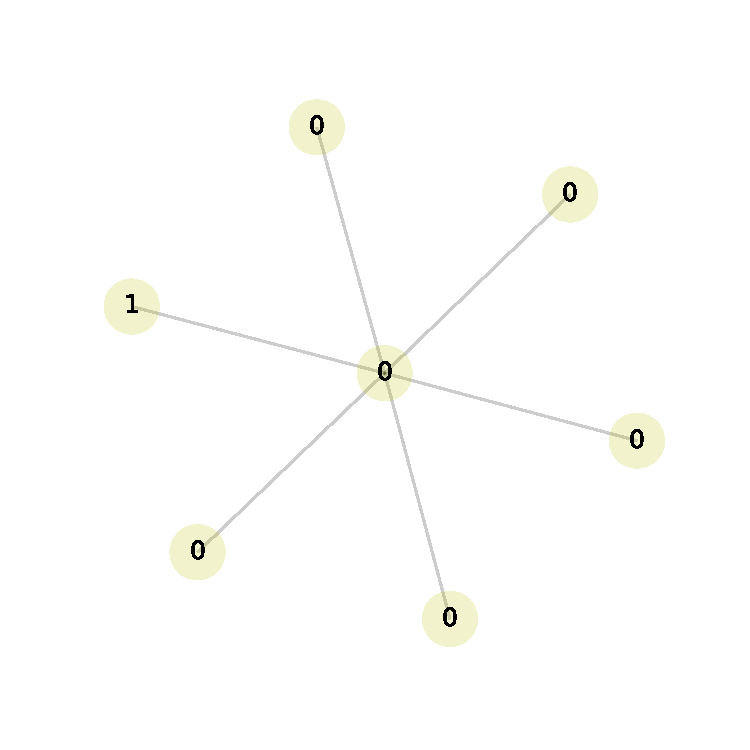
\includegraphics[scale=0.4]{../Figures/star_no_alpha_update_abs_value.pdf}\end{center}
%% \end{column}
%% \begin{column}{0.45\textwidth}
%% \vspace{20pt}
%% Only the center node with value 0 and the leaf node with value 1 can update. If they perform an $\alpha$-update, the sum of their $f$-discordances increases from $$|1-0|+|0-1|=2$$ to
%% \begin{equation*}
%% \begin{aligned}
%%     |(1-\alpha)-\alpha|\\
%%     +|\alpha-(1-\alpha)|\\
%%     +5|\alpha-0| = 2+\alpha.
%% \end{aligned}
%% \end{equation*}
%% \end{column}
%% \end{columns}
%% \end{minipage}
%% \end{frame}
%
%
%
%
%% %%%%% Establish we are working with f(t)=t^2
%
%
%% \begin{frame}{Condition for Pairwise Compromise}
%% Hence, let us restrict our attention to the case where $f(t)=t^2$. \\~\\
%
%% Two nodes $p$ and $q$, where $x_p>x_q$, are able to come to a pairwise compromise, i.e. update both of their values to the mean $\dfrac{x_p+x_q}{2}$, if and only if:
%
%% \begin{equation}\label{eqn:meetmiddleinequality}
%%       \sum_{\substack{k=1\\k\neq q}}^nA_{pk}  (x_k-x_p)
%% 	    + \sum_{\substack{k=1\\k\neq p}}^nA_{qk}  (x_q-x_k) 
%% 	    < \left(4 -\dfrac{6 + k_p+k_q}{4}\right)  \left(x_p-x_q\right).
%% \end{equation} \\ ~\\
%
%% From this inequality, one can prove that for any configuration of the complete network that any two nodes with distinct values can come to a pairwise compromise.
%% \end{frame}
%
%
%% \begin{frame}{Classifying Networks}
%% Call a connected network \emph{$2$-friendly} if for any nontrivial configuration there always exists a pair of adjacent nodes that can come to a pairwise compromise. \\ ~\\
%
%% Because the condition for existence of a pairwise compromise is a linear inequality, we can classify 2-friendly networks using a sequence of Linear Programming solves. 
%% \end{frame}
%
%
%% \begin{frame}{Classifying Networks}
%% Cycle and Star Networks \\
%% A cycle network with $\leq 8$ nodes is 2-friendly, while cycles with $\geq 9$ nodes are not. A star network with $\leq 4$ leaf nodes is 2-friendly, while stars with $\geq 5$ leaf nodes are not. Examples of stalemate configurations:
%
%% \begin{figure}[!tbp]
%%   \centering
%%   \begin{minipage}[b]{0.35\textwidth}
%%     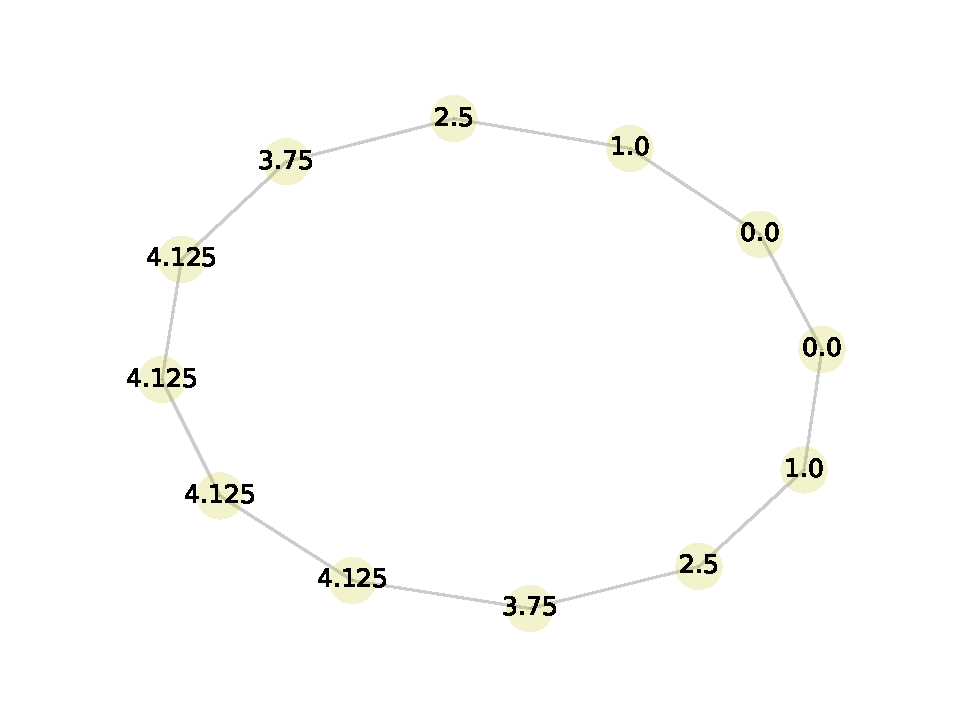
\includegraphics[scale=0.35]{../Figures/success_graph_with_12_nodes_code_9.pdf}
%%     \caption{Cycle Network}
%%   \end{minipage}
%%   \hfill
%%   \begin{minipage}[b]{0.4\textwidth}
%%     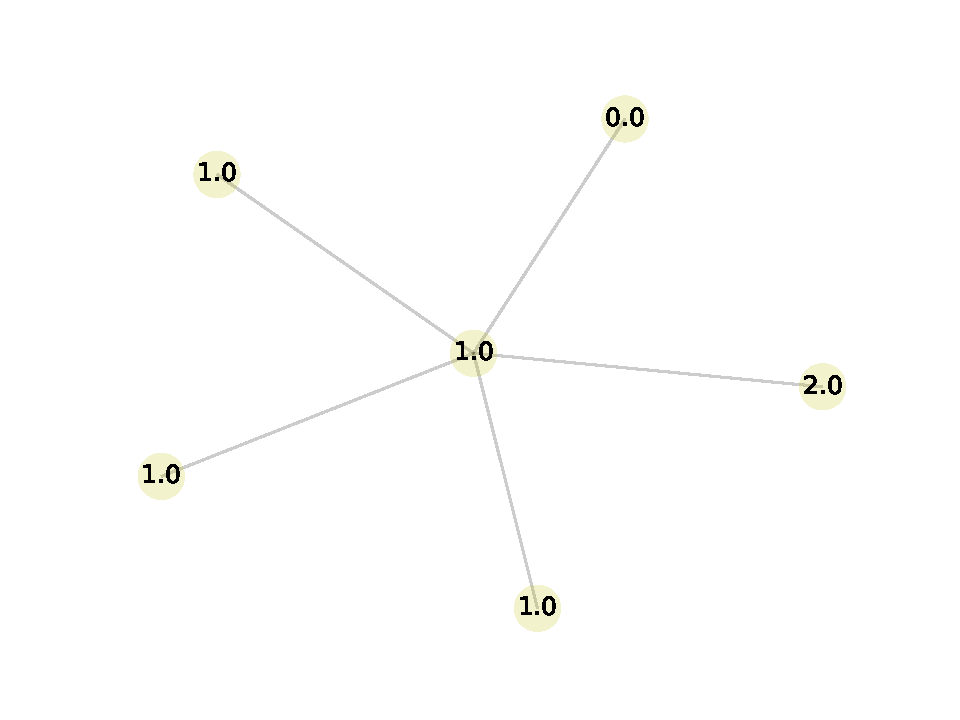
\includegraphics[scale=0.3]{../Figures/success_graph_with_6_nodes_code_29.pdf}
%%     \caption{Star Network}
%%   \end{minipage}
%% \end{figure}
%% \end{frame}
%
%
%
%% \begin{frame}{Building non-2-friendly networks}
%% Let $G$ be a connected, non-2-friendly network on $n$ nodes and let $\{H_i\}_{i=1}^m$ be $m$ arbitrary connected networks. Connect each $H_i$ to exactly one node in $G$, either through one or multiple edges. The resulting graph is connected and non-2-friendly. We can use this to show when we have a path graph of length $k$ which is non-2-friendly, all longer path graphs are also non-2-friendly. 
%
%
%
%% \begin{figure}[!tbp]
%%   \centering
%%   \begin{minipage}[b]{0.35\textwidth}
%%     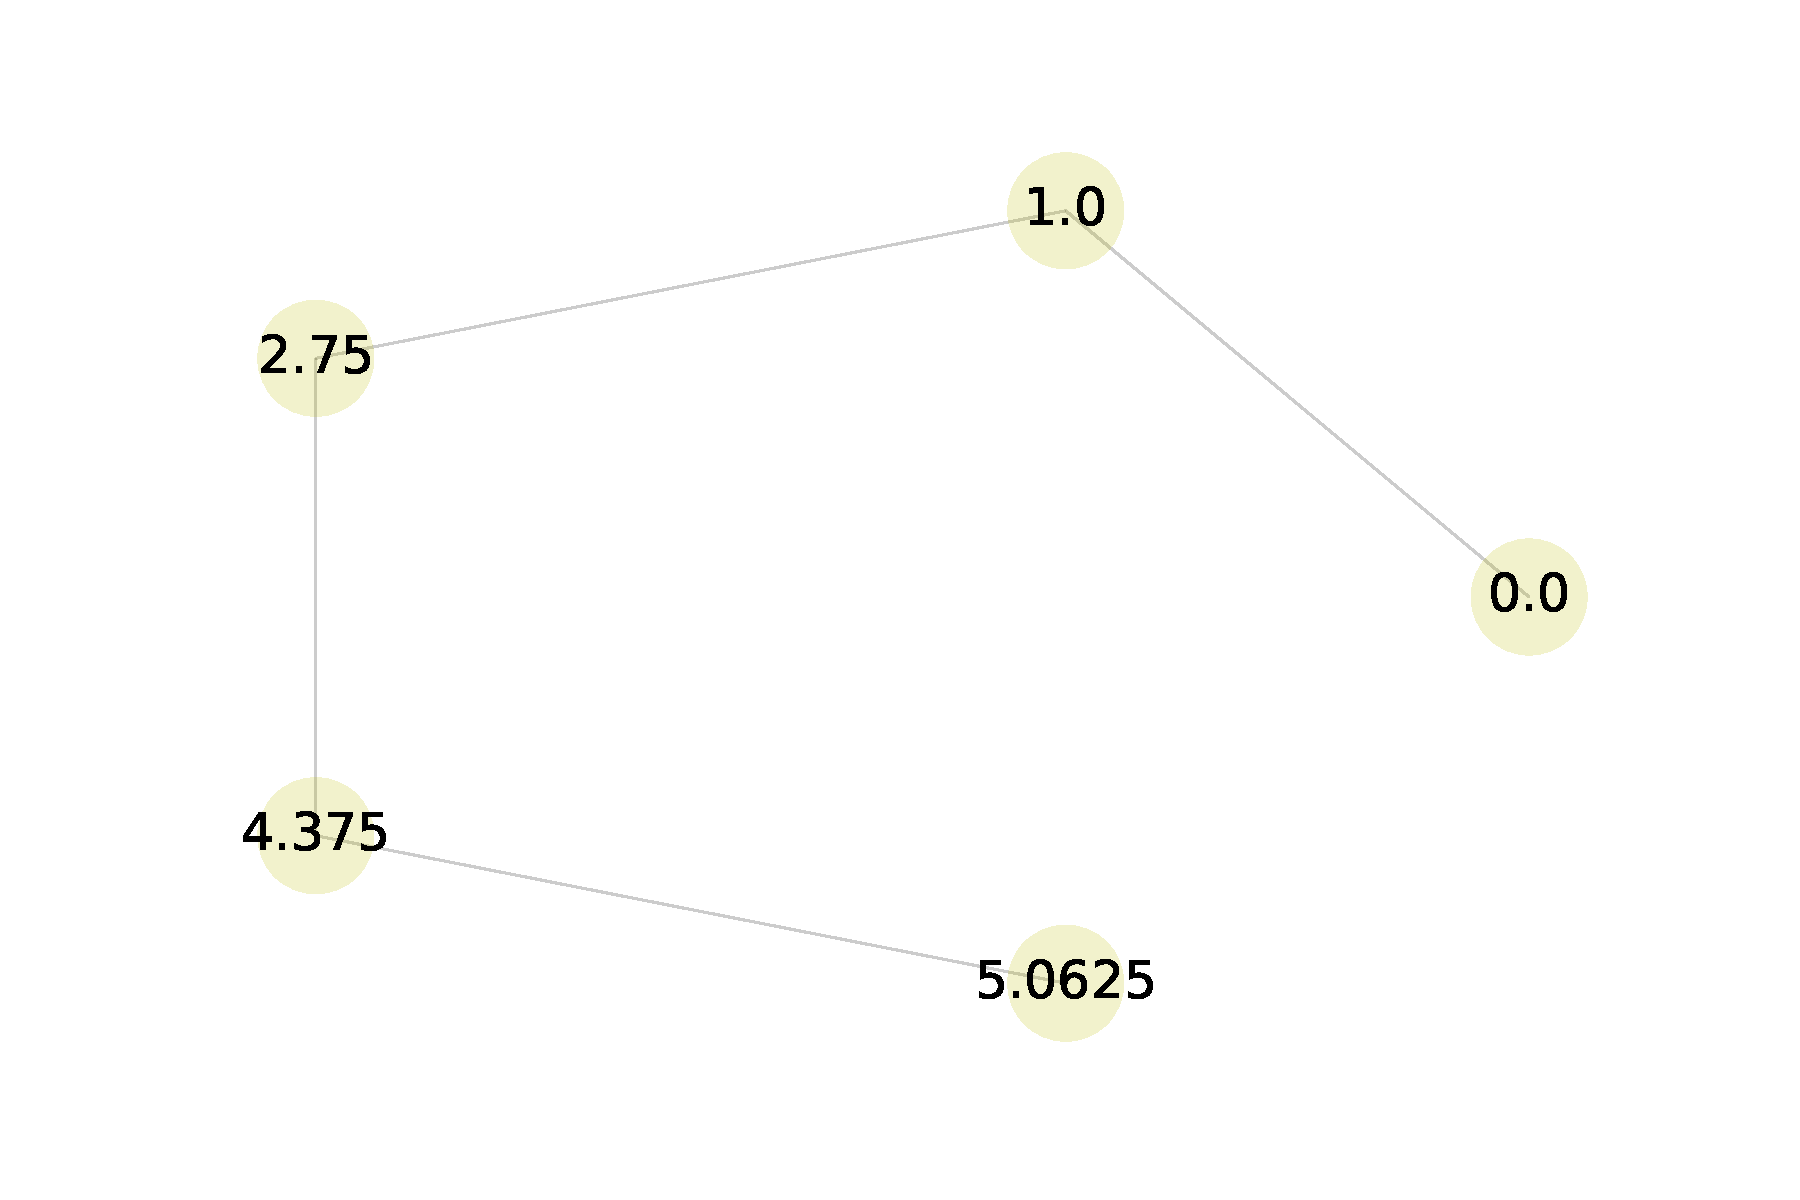
\includegraphics[scale=0.15]{../Figures/success_graph_with_5_nodes_code_path_5.pdf}
%%     \caption{Path}
%%   \end{minipage}
%%   \hfill
%%   \begin{minipage}[b]{0.4\textwidth}
%%     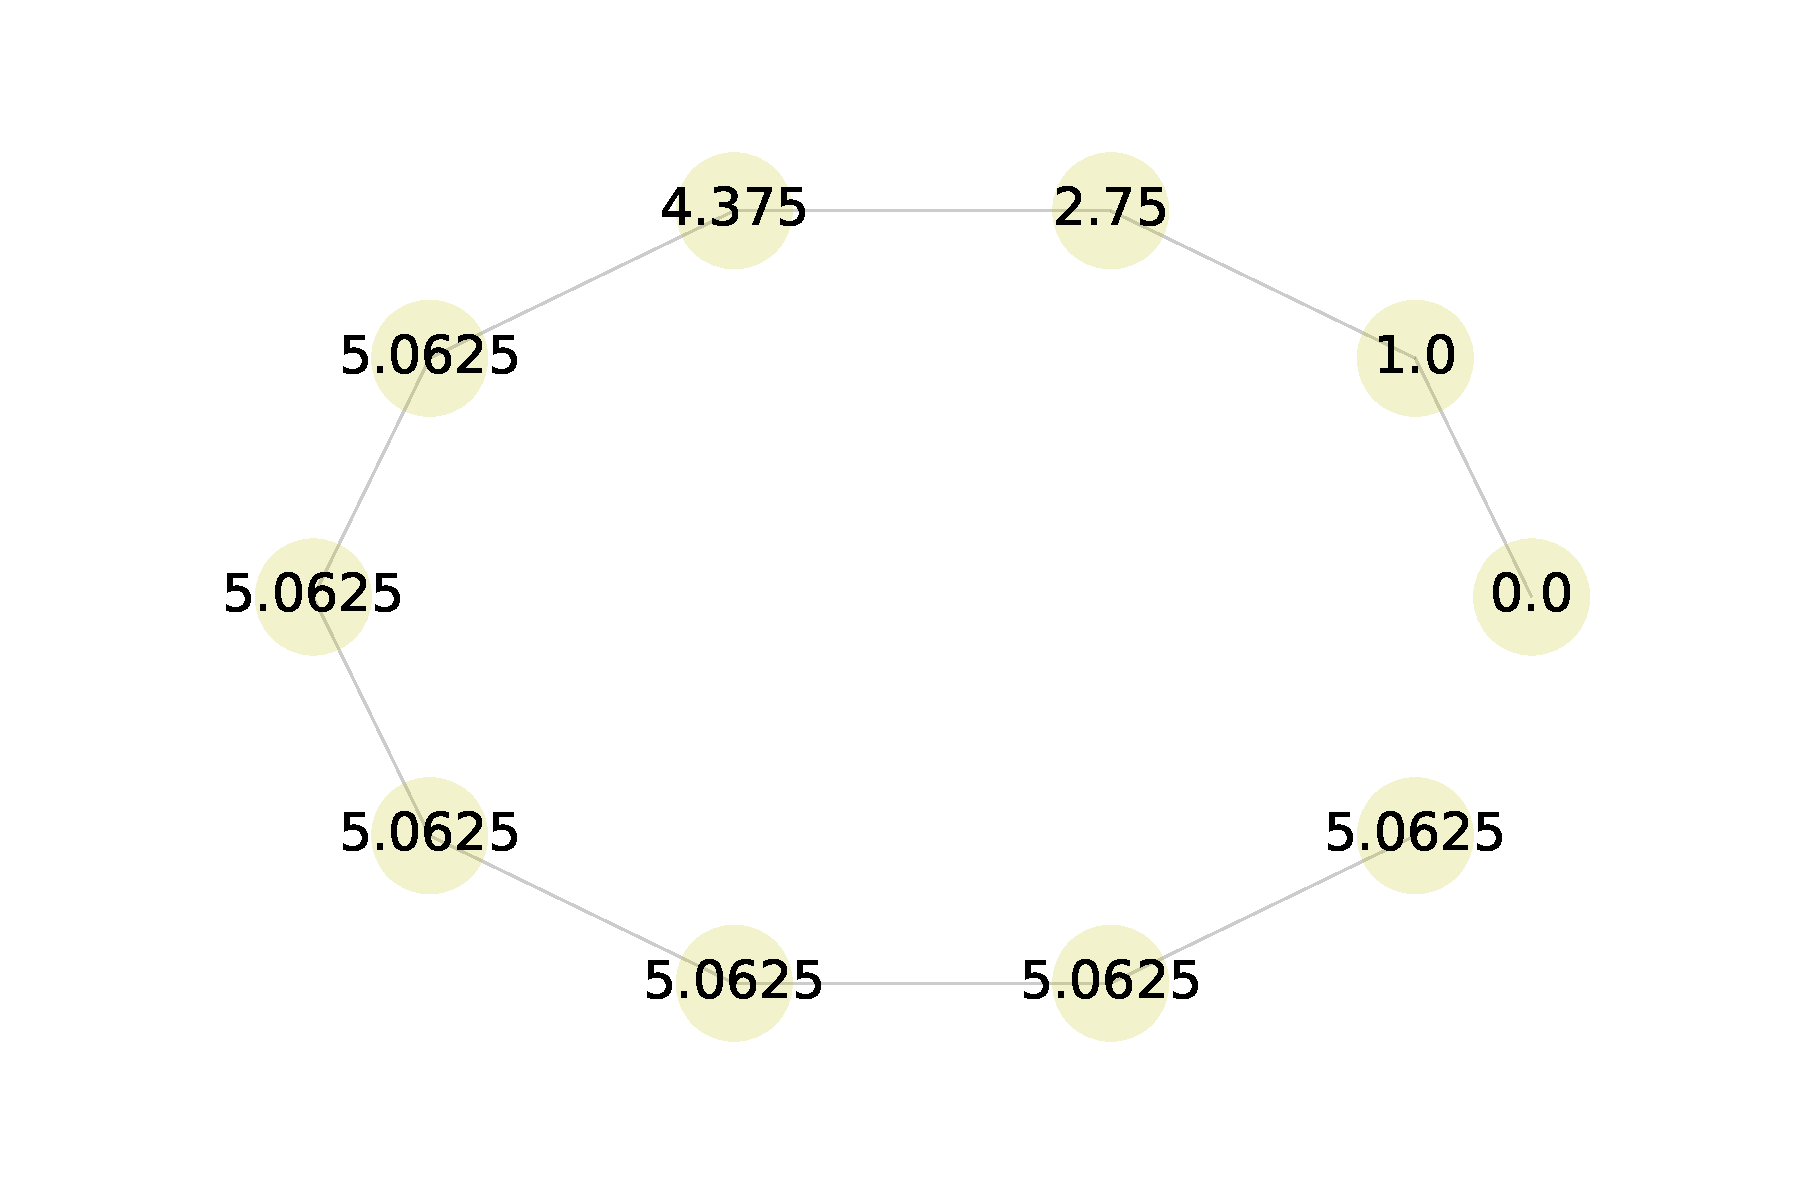
\includegraphics[scale=0.15]{../Figures/success_graph_with_10_nodes_code_path_10.pdf}
%%     \caption{Longer Path}
%%   \end{minipage}
%% \end{figure}
%% \end{frame}
%
%
%
%
%
%
%% \begin{frame}{Some results on $k$-friendly networks}
%% Call a connected network \emph{$k$-friendly} if for any nontrivial configuration there always exists a connected subgraph $S$ with $k$ nodes that can come to a $k$-wise compromise, i.e. update the values of all nodes in $S$ to the mean $\dfrac{1}{k}\displaystyle \sum_{v\in S} x_v.$ \\ ~\\
%% \begin{center}
%%     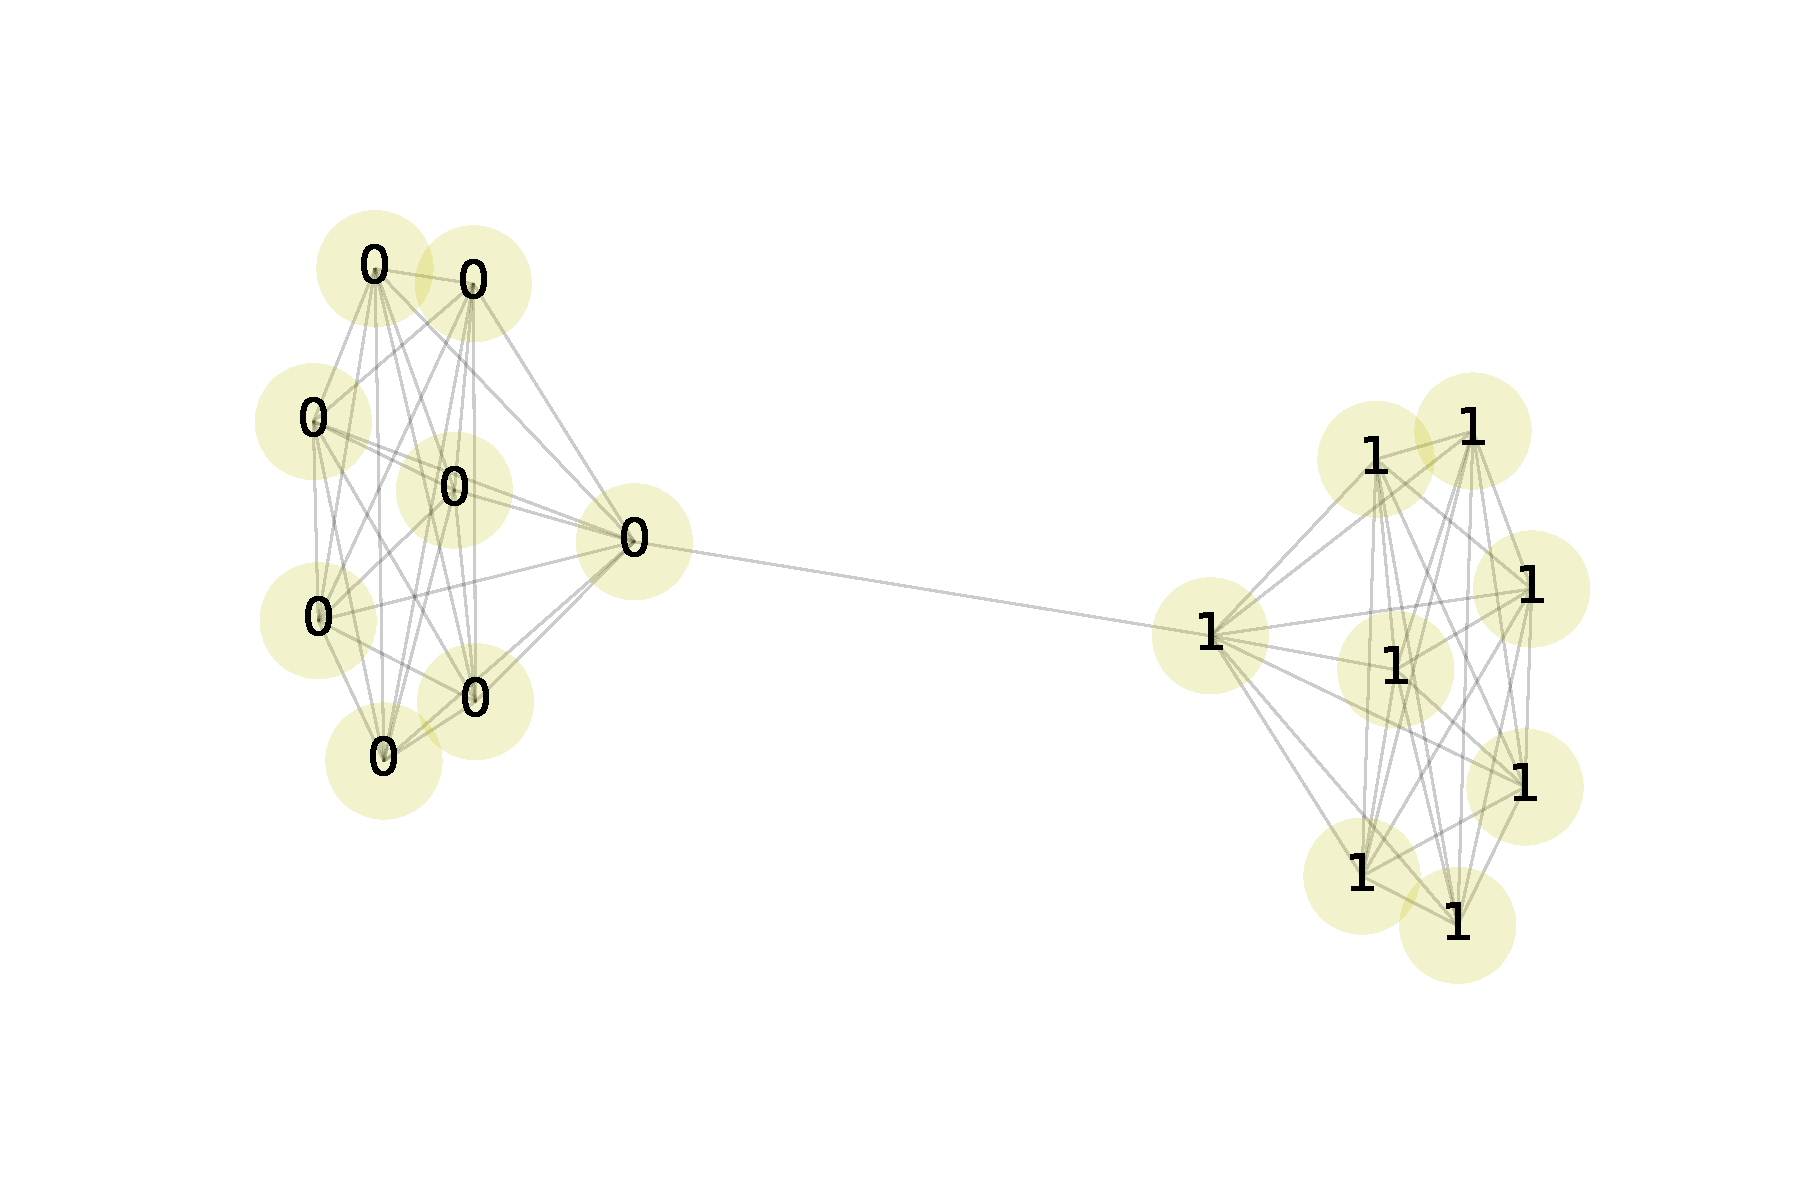
\includegraphics[scale=0.25]{../Figures/barbell.pdf}
%% \end{center}
%
%
%% \end{frame}
%
%
%
%
%
%% \begin{frame}{Conclusion}
%
%% \end{frame}
%
%
%% \begin{frame}{Future Work}
%% \begin{itemize}
%%     \item Is the class of non-2-friendly networks closed under subdivision? That is, if $G$ is a non-2-friendly network and $H$ is obtained from $G$ via a sequence of subdivisions, is $H$ also non-2-friendly?
%% \end{itemize}
%% \end{frame}
%
%
%
%% \begin{frame}[allowframebreaks]
%% {References}
%
%% % \nocite{*}
%% \bibliographystyle{unsrt}
%% \bibliography{}
%
%% \end{frame}
%





\end{document}
